% Options for packages loaded elsewhere
\PassOptionsToPackage{unicode}{hyperref}
\PassOptionsToPackage{hyphens}{url}
%
\documentclass[
]{book}
\usepackage{amsmath,amssymb}
\usepackage{lmodern}
\usepackage{ifxetex,ifluatex}
\ifnum 0\ifxetex 1\fi\ifluatex 1\fi=0 % if pdftex
  \usepackage[T1]{fontenc}
  \usepackage[utf8]{inputenc}
  \usepackage{textcomp} % provide euro and other symbols
\else % if luatex or xetex
  \usepackage{unicode-math}
  \defaultfontfeatures{Scale=MatchLowercase}
  \defaultfontfeatures[\rmfamily]{Ligatures=TeX,Scale=1}
\fi
% Use upquote if available, for straight quotes in verbatim environments
\IfFileExists{upquote.sty}{\usepackage{upquote}}{}
\IfFileExists{microtype.sty}{% use microtype if available
  \usepackage[]{microtype}
  \UseMicrotypeSet[protrusion]{basicmath} % disable protrusion for tt fonts
}{}
\makeatletter
\@ifundefined{KOMAClassName}{% if non-KOMA class
  \IfFileExists{parskip.sty}{%
    \usepackage{parskip}
  }{% else
    \setlength{\parindent}{0pt}
    \setlength{\parskip}{6pt plus 2pt minus 1pt}}
}{% if KOMA class
  \KOMAoptions{parskip=half}}
\makeatother
\usepackage{xcolor}
\IfFileExists{xurl.sty}{\usepackage{xurl}}{} % add URL line breaks if available
\IfFileExists{bookmark.sty}{\usepackage{bookmark}}{\usepackage{hyperref}}
\hypersetup{
  pdftitle={Learning statistics with jamovi: a tutorial for psychology students and other beginners (Version 0.70)},
  pdfauthor={Danielle Navarro and David Foxcroft},
  hidelinks,
  pdfcreator={LaTeX via pandoc}}
\urlstyle{same} % disable monospaced font for URLs
\usepackage{color}
\usepackage{fancyvrb}
\newcommand{\VerbBar}{|}
\newcommand{\VERB}{\Verb[commandchars=\\\{\}]}
\DefineVerbatimEnvironment{Highlighting}{Verbatim}{commandchars=\\\{\}}
% Add ',fontsize=\small' for more characters per line
\usepackage{framed}
\definecolor{shadecolor}{RGB}{248,248,248}
\newenvironment{Shaded}{\begin{snugshade}}{\end{snugshade}}
\newcommand{\AlertTok}[1]{\textcolor[rgb]{0.94,0.16,0.16}{#1}}
\newcommand{\AnnotationTok}[1]{\textcolor[rgb]{0.56,0.35,0.01}{\textbf{\textit{#1}}}}
\newcommand{\AttributeTok}[1]{\textcolor[rgb]{0.77,0.63,0.00}{#1}}
\newcommand{\BaseNTok}[1]{\textcolor[rgb]{0.00,0.00,0.81}{#1}}
\newcommand{\BuiltInTok}[1]{#1}
\newcommand{\CharTok}[1]{\textcolor[rgb]{0.31,0.60,0.02}{#1}}
\newcommand{\CommentTok}[1]{\textcolor[rgb]{0.56,0.35,0.01}{\textit{#1}}}
\newcommand{\CommentVarTok}[1]{\textcolor[rgb]{0.56,0.35,0.01}{\textbf{\textit{#1}}}}
\newcommand{\ConstantTok}[1]{\textcolor[rgb]{0.00,0.00,0.00}{#1}}
\newcommand{\ControlFlowTok}[1]{\textcolor[rgb]{0.13,0.29,0.53}{\textbf{#1}}}
\newcommand{\DataTypeTok}[1]{\textcolor[rgb]{0.13,0.29,0.53}{#1}}
\newcommand{\DecValTok}[1]{\textcolor[rgb]{0.00,0.00,0.81}{#1}}
\newcommand{\DocumentationTok}[1]{\textcolor[rgb]{0.56,0.35,0.01}{\textbf{\textit{#1}}}}
\newcommand{\ErrorTok}[1]{\textcolor[rgb]{0.64,0.00,0.00}{\textbf{#1}}}
\newcommand{\ExtensionTok}[1]{#1}
\newcommand{\FloatTok}[1]{\textcolor[rgb]{0.00,0.00,0.81}{#1}}
\newcommand{\FunctionTok}[1]{\textcolor[rgb]{0.00,0.00,0.00}{#1}}
\newcommand{\ImportTok}[1]{#1}
\newcommand{\InformationTok}[1]{\textcolor[rgb]{0.56,0.35,0.01}{\textbf{\textit{#1}}}}
\newcommand{\KeywordTok}[1]{\textcolor[rgb]{0.13,0.29,0.53}{\textbf{#1}}}
\newcommand{\NormalTok}[1]{#1}
\newcommand{\OperatorTok}[1]{\textcolor[rgb]{0.81,0.36,0.00}{\textbf{#1}}}
\newcommand{\OtherTok}[1]{\textcolor[rgb]{0.56,0.35,0.01}{#1}}
\newcommand{\PreprocessorTok}[1]{\textcolor[rgb]{0.56,0.35,0.01}{\textit{#1}}}
\newcommand{\RegionMarkerTok}[1]{#1}
\newcommand{\SpecialCharTok}[1]{\textcolor[rgb]{0.00,0.00,0.00}{#1}}
\newcommand{\SpecialStringTok}[1]{\textcolor[rgb]{0.31,0.60,0.02}{#1}}
\newcommand{\StringTok}[1]{\textcolor[rgb]{0.31,0.60,0.02}{#1}}
\newcommand{\VariableTok}[1]{\textcolor[rgb]{0.00,0.00,0.00}{#1}}
\newcommand{\VerbatimStringTok}[1]{\textcolor[rgb]{0.31,0.60,0.02}{#1}}
\newcommand{\WarningTok}[1]{\textcolor[rgb]{0.56,0.35,0.01}{\textbf{\textit{#1}}}}
\usepackage{longtable,booktabs,array}
\usepackage{calc} % for calculating minipage widths
% Correct order of tables after \paragraph or \subparagraph
\usepackage{etoolbox}
\makeatletter
\patchcmd\longtable{\par}{\if@noskipsec\mbox{}\fi\par}{}{}
\makeatother
% Allow footnotes in longtable head/foot
\IfFileExists{footnotehyper.sty}{\usepackage{footnotehyper}}{\usepackage{footnote}}
\makesavenoteenv{longtable}
\usepackage{graphicx}
\makeatletter
\def\maxwidth{\ifdim\Gin@nat@width>\linewidth\linewidth\else\Gin@nat@width\fi}
\def\maxheight{\ifdim\Gin@nat@height>\textheight\textheight\else\Gin@nat@height\fi}
\makeatother
% Scale images if necessary, so that they will not overflow the page
% margins by default, and it is still possible to overwrite the defaults
% using explicit options in \includegraphics[width, height, ...]{}
\setkeys{Gin}{width=\maxwidth,height=\maxheight,keepaspectratio}
% Set default figure placement to htbp
\makeatletter
\def\fps@figure{htbp}
\makeatother
\setlength{\emergencystretch}{3em} % prevent overfull lines
\providecommand{\tightlist}{%
  \setlength{\itemsep}{0pt}\setlength{\parskip}{0pt}}
\setcounter{secnumdepth}{5}
\usepackage{booktabs}
\ifluatex
  \usepackage{selnolig}  % disable illegal ligatures
\fi
\usepackage[]{natbib}
\bibliographystyle{apalike}

\title{Learning statistics with jamovi: a tutorial for psychology students and other beginners (Version 0.70)}
\author{Danielle Navarro and David Foxcroft}
\date{2021-09-14}

\begin{document}
\maketitle

{
\setcounter{tocdepth}{1}
\tableofcontents
}
\hypertarget{overview}{%
\chapter*{Overview}\label{overview}}
\addcontentsline{toc}{chapter}{Overview}

\emph{learning statistics with jamovi} covers the contents of an introductory statistics class, as typically taught to undergraduate psychology students. The book discusses how to get started in jamovi as well as giving an introduction to data manipulation. From a statistical perspective, the book discusses descriptive statistics and graphing first, followed by chapters on probability theory, sampling and estimation, and null hypothesis testing. After introducing the theory, the book covers the analysis of contingency tables, correlation, \(t\)-tests, regression, ANOVA and factor analysis. Bayesian statistics are covered at the end of the book.

\hypertarget{citation}{%
\chapter*{Citation}\label{citation}}
\addcontentsline{toc}{chapter}{Citation}

Navarro DJ and Foxcroft DR (2019). learning statistics with jamovi: a tutorial for psychology students and other beginners. (Version 0.70). DOI: 10.24384/hgc3-7p15 {[}Available from url: \url{http://learnstatswithjamovi.com}{]}

\hypertarget{licensing}{%
\chapter*{Licensing}\label{licensing}}
\addcontentsline{toc}{chapter}{Licensing}

This book is published under a Creative Commons BY-SA license (CC BY-SA) version 4.0. This means that this book can be reused, remixed, retained, revised and redistributed (including commercially) as long as appropriate credit is given to the authors. If you remix, or modify the original version of this open textbook, you must redistribute all versions of this open textbook under the same license - CC BY-SA. \url{https://creativecommons.org/licenses/by-sa/4.0/}

\hypertarget{dedication}{%
\chapter*{Dedication}\label{dedication}}
\addcontentsline{toc}{chapter}{Dedication}

\emph{This book was brought to you today by the letter `R' and the word `jamovi'}

\hypertarget{preface}{%
\chapter*{Preface}\label{preface}}
\addcontentsline{toc}{chapter}{Preface}

\hypertarget{preface-to-version-0.70}{%
\section{Preface to Version 0.70}\label{preface-to-version-0.70}}

This update from version 0.65 introduces some new analyses. In the ANOVA chapters we have added sections on repeated measures ANOVA and analysis of covariance (ANCOVA). In a new chapter we have introduced Factor Analysis and related techniques. Hopefully the style of this new material is consistent with the rest of the book, though eagle-eyed readers might spot a bit more of an emphasis on conceptual and practical explanations, and a bit less algebra. I'm not sure this is a good thing, and might add the algebra in a bit later. But it reflects both my approach to understanding and teaching statistics, and also some feedback I have received from students on a course I teach. In line with this, I have also been through the rest of the book and tried to separate out some of the algebra by putting it into a box or frame. It's not that this stuff is not important or useful, but for some students they may wish to skip over it and therefore the boxing of these parts should help some readers.

With this version I am very grateful to comments and feedback received from my students and colleagues, notably Wakefield Morys-Carter, and also to numerous people all over the world who have sent in small suggestions and corrections - much appreciated, and keep them coming! One pretty neat new feature is that the example data files for the book can now be loaded into jamovi as an add-on module - thanks to Jonathon Love for helping with that.

David Foxcroft
February 1st, 2019

\hypertarget{preface-to-version-0.65}{%
\section{Preface to Version 0.65}\label{preface-to-version-0.65}}

In this adaptation of the excellent `Learning statistics with R', by Danielle Navarro, we have replaced the statistical software used for the analyses and examples with jamovi. Although R is a powerful statistical programming language, it is not the first choice for every instructor and student at the beginning of their statistical learning. Some instructors and students tend to prefer the point-and-click style of software, and that's where jamovi comes in. jamovi is software that aims to simplify two aspects of using R. It offers a point-and-click graphical user interface (GUI), and it also provides functions that combine the capabilities of many others, bringing a more SPSS- or SAS-like method of programming to R. Importantly, jamovi will always be free and open - that's one of its core values - because jamovi is made by the scientific community, for the scientific community.

With this version I am very grateful for the help of others who have read through drafts and provided excellent suggestions and corrections, particularly Dr David Emery and Kirsty Walter.

David Foxcroft
July 1st, 2018

\hypertarget{preface-to-version-0.6}{%
\section{Preface to Version 0.6}\label{preface-to-version-0.6}}

The book hasn't changed much since 2015 when I released Version 0.5 -- it's probably fair to say that I've changed more than it has. I moved from Adelaide to Sydney in 2016 and my teaching profile at UNSW is different to what it was at Adelaide, and I haven't really had a chance to work on it since arriving here! It's a little strange looking back at this actually. A few quick comments\ldots{}

\begin{itemize}
\tightlist
\item
  Weirdly, the book \emph{consistently} misgenders me, but I suppose I have only myself to blame for that one :-) There's now a brief footnote on page 12 that mentions this issue; in real life I've been working through a gender affirmation process for the last two years and mostly go by she/her pronouns. I am, however, just as lazy as I ever was so I haven't bothered updating the text in the book.\\
\item
  For Version 0.6 I haven't changed much I've made a few minor changes when people have pointed out typos or other errors. In particular it's worth noting the issue associated with the etaSquared function in the \textbf{lsr} package (which isn't really being maintained any more) in Section 14.4. The function works fine for the simple examples in the book, but there are definitely bugs in there that I haven't found time to check! So please take care with that one.
\item
  The biggest change really is the licensing! I've released it under a Creative Commons licence (CC BY-SA 4.0, specifically), and placed all the source files to the associated GitHub repository, if anyone wants to adapt it.
\end{itemize}

Maybe someone would like to write a version that makes use of the \textbf{tidyverse}\ldots{} I hear that's become rather important to R these days :-)

Best,
Danielle Navarro

\hypertarget{preface-to-version-0.5}{%
\section{Preface to Version 0.5}\label{preface-to-version-0.5}}

Another year, another update. This time around, the update has focused almost entirely on the theory sections of the book. Chapters 9, 10 and 11 have been rewritten, hopefully for the better. Along the same lines, Chapter 17 is entirely new, and focuses on Bayesian statistics. I think the changes have improved the book a great deal. I've always felt uncomfortable about the fact that all the inferential statistics in the book are presented from an orthodox perspective, even though I almost always present Bayesian data analyses in my own work. Now that I've managed to squeeze Bayesian methods into the book somewhere, I'm starting to feel better about the book as a whole. I wanted to get a few other things done in this update, but as usual I'm running into teaching deadlines, so the update has to go out the way it is!

Dan Navarro
February 16, 2015

\hypertarget{preface-to-version-0.4}{%
\section{Preface to Version 0.4}\label{preface-to-version-0.4}}

A year has gone by since I wrote the last preface. The book has changed in a few important ways: Chapters 3 and 4 do a better job of documenting some of the time saving features of Rstudio, Chapters 12 and 13 now make use of new functions in the lsr package for running chi-square tests and t tests, and the discussion of correlations has been adapted to refer to the new functions in the lsr package. The soft copy of 0.4 now has better internal referencing (i.e., actual hyperlinks between sections), though that was introduced in 0.3.1. There's a few tweaks here and there, and many typo corrections (thank you to everyone who pointed out typos!), but overall 0.4 isn't massively different from 0.3.

I wish I'd had more time over the last 12 months to add more content. The absence of any discussion of repeated measures ANOVA and mixed models more generally really does annoy me. My excuse for this lack of progress is that my second child was born at the start of 2013, and so I spent most of last year just trying to keep my head above water. As a consequence, unpaid side projects like this book got sidelined in favour of things that actually pay my salary! Things are a little calmer now, so with any luck version 0.5 will be a bigger step forward.

One thing that has surprised me is the number of downloads the book gets. I finally got some basic tracking information from the website a couple of months ago, and (after excluding obvious robots) the book has been averaging about 90 downloads per day. That's encouraging: there's at least a few people who find the book useful!

Dan Navarro
February 4, 2014

\hypertarget{preface-to-version-0.3}{%
\section{Preface to Version 0.3}\label{preface-to-version-0.3}}

There's a part of me that really \textbf{doesn't} want to publish this book. It's not finished.

And when I say that, I mean it. The referencing is spotty at best, the chapter summaries are just lists of section titles, there's no index, there are no exercises for the reader, the organisation is suboptimal, and the coverage of topics is just not comprehensive enough for my liking. Additionally, there are sections with content that I'm not happy with, figures that really need to be redrawn, and I've had almost no time to hunt down inconsistencies, typos, or errors. In other words, \emph{this book is not finished}. If I didn't have a looming teaching deadline and a baby due in a few weeks, I really wouldn't be making this available at all.

What this means is that if you are an academic looking for teaching materials, a Ph.D.~student looking to learn R, or just a member of the general public interested in statistics, I would advise you to be cautious. What you're looking at is a first draft, and it may not serve your purposes. If we were living in the days when publishing was expensive and the internet wasn't around, I would never consider releasing a book in this form. The thought of someong shelling out \$80 for this (which is what a commercial publisher told me it would retail for when they offered to distribute it) makes me feel more than a little uncomfortable. However, it's the 21st century, so I can post the pdf on my website for free, and I can distribute hard copies via a print-on-demand service for less than half what a textbook publisher would charge. And so my guilt is assuaged, and I'm willing to share! With that in mind, you can obtain free soft copies and cheap hard copies online, from the following webpages:

\begin{itemize}
\tightlist
\item
  \url{http://www.compcogscisydney.com/learning-statistics-with-r.html}
\item
  \url{http://www.lulu.com/content/13570633}
\end{itemize}

Even so, the warning still stands: what you are looking at is Version 0.3 of a work in progress. If and when it hits Version 1.0, I would be willing to stand behind the work and say, yes, this is a textbook that I would encourage other people to use. At that point, I'll probably start shamelessly flogging the thing on the internet and generally acting like a tool. But until that day comes, I'd like it to be made clear that I'm really ambivalent about the work as it stands.

All of the above being said, there is one group of people that I can enthusiastically endorse this book to: the psychology students taking our undergraduate research methods classes (DRIP and DRIP:A) in 2013. For you, this book is ideal, because it was written to accompany your stats lectures. If a problem arises due to a shortcoming of these notes, I can and will adapt content on the fly to fix that problem. Effectively, you've got a textbook written specifically for your classes, distributed for free (electronic copy) or at near-cost prices (hard copy). Better yet, the notes have been tested: Version 0.1 of these notes was used in the 2011 class, Version 0.2 was used in the 2012 class, and now you're looking at the new and improved Version 0.3. I'm not saying these notes are titanium plated awesomeness on a stick -- though if \emph{you} wanted to say so on the student evaluation forms, then you're totally welcome to -- because they're not. But I am saying that they've been tried out in previous years and they seem to work okay. Besides, there's a group of us around to troubleshoot if any problems come up, and you can guarantee that at least \emph{one} of your lecturers has read the whole thing cover to cover!

Okay, with all that out of the way, I should say something about what the book aims to be. At its core, it is an introductory statistics textbook pitched primarily at psychology students. As such, it covers the standard topics that you'd expect of such a book: study design, descriptive statistics, the theory of hypothesis testing, \(t\)-tests, \(\chi^2\) tests, ANOVA and regression. However, there are also several chapters devoted to the R statistical package, including a chapter on data manipulation and another one on scripts and programming. Moreover, when you look at the content presented in the book, you'll notice a lot of topics that are traditionally swept under the carpet when teaching statistics to psychology students. The Bayesian/frequentist divide is openly disussed in the probability chapter, and the disagreement between Neyman and Fisher about hypothesis testing makes an appearance. The difference between probability and density is discussed. A detailed treatment of Type I, II and III sums of squares for unbalanced factorial ANOVA is provided. And if you have a look in the Epilogue, it should be clear that my intention is to add a lot more advanced content.

My reasons for pursuing this approach are pretty simple: the students can handle it, and they even seem to enjoy it. Over the last few years I've been pleasantly surprised at just how little difficulty I've had in getting undergraduate psych students to learn R. It's certainly not easy for them, and I've found I need to be a little charitable in setting marking standards, but they do eventually get there. Similarly, they don't seem to have a lot of problems tolerating ambiguity and complexity in presentation of statistical ideas,
as long as they are assured that the assessment standards will be set in a fashion that is appropriate for them. So if the students can handle it, why \emph{not} teach it? The potential gains are pretty enticing. If they learn R, the students get access to CRAN, which is perhaps the largest and most comprehensive library of statistical tools in existence. And if they learn about probability theory in detail, it's easier for them to switch from orthodox null hypothesis testing to Bayesian methods if they want to. Better yet, they learn data analysis skills that they can take to an employer without being dependent on expensive and proprietary software.

Sadly, this book isn't the silver bullet that makes all this possible. It's a work in progress, and maybe when it is finished it will be a useful tool. One among many, I would think. There are a number of other books that try to provide a basic introduction to statistics using R, and I'm not arrogant enough to believe that mine is better. Still, I rather like the book, and maybe other people will find it useful, incomplete though it is.

Dan Navarro
January 13, 2013

\hypertarget{part-i.-background}{%
\chapter*{Part I. Background}\label{part-i.-background}}
\addcontentsline{toc}{chapter}{Part I. Background}

\hypertarget{why-do-we-learn-statistics}{%
\chapter{Why do we learn statistics?}\label{why-do-we-learn-statistics}}

\begin{quote}
``Thou shalt not answer questionnaires\\
Or quizzes upon World Affairs,
Nor with compliance\\
Take any test. Thou shalt not sit\\
With statisticians nor commit''
-- W.H. Auden\footnote{The quote comes from Auden's 1946 poem \emph{Under Which Lyre: A Reactionary Tract for the Times}, delivered as part of a commencement address at Harvard University. The history of the poem is kind of interesting: \url{http://harvardmagazine.com/2007/11/a-poets-warning.html}}
\end{quote}

\hypertarget{whywhywhy}{%
\section{On the psychology of statistics}\label{whywhywhy}}

To the surprise of many students, statistics is a fairly significant part of a psychological education. To the surprise of no-one, statistics is very rarely the \emph{favourite} part of one's psychological education. After all, if you really loved the idea of doing statistics, you'd probably be enrolled in a statistics class right now, not a psychology class. So, not surprisingly, there's a pretty large proportion of the student base that isn't happy about the fact that psychology has so much statistics in it. In view of this, I thought that the right place to start might be to answer some of the more common questions that people have about stats.

A big part of this issue at hand relates to the very idea of statistics. What is it? What's it there for? And why are scientists so bloody obsessed with it? These are all good questions, when you think about it. So let's start with the last one. As a group, scientists seem to be bizarrely fixated on running statistical tests on everything. In fact, we use statistics so often that we sometimes forget to explain to people why we do. It's a kind of article of faith among scientists -- and especially social scientists -- that your findings can't be trusted until you've done some stats. Undergraduate students might be forgiven for thinking that we're all completely mad, because no-one takes the time to answer one very simple question:

\begin{quote}
\emph{Why do you do statistics? Why don't scientists just use \textbf{common sense?}}
\end{quote}

It's a naive question in some ways, but most good questions are. There's a lot of good answers to it,\footnote{Including the suggestion that common sense is in short supply among scientists.} but for my money, the best answer is a really simple one: we don't trust ourselves enough. We worry that we're human, and susceptible to all of the biases, temptations and frailties that humans suffer from. Much of statistics is basically a safeguard. Using ``common sense'' to evaluate evidence means trusting gut instincts, relying on verbal arguments and on using the raw power of human reason to come up with the right answer. Most scientists don't think this approach is likely to work.

In fact, come to think of it, this sounds a lot like a psychological question to me, and since I do work in a psychology department, it seems like a good idea to dig a little deeper here. Is it really plausible to think that this ``common sense'' approach is very trustworthy? Verbal arguments have to be constructed in language, and all languages have biases -- some things are harder to say than others, and not necessarily because they're false (e.g., quantum electrodynamics is a good theory, but hard to explain in words). The instincts of our ``gut'' aren't designed to solve scientific problems, they're designed to handle day to day inferences -- and given that biological evolution is slower than cultural change, we should say that they're designed to solve the day to day problems for a \emph{different world} than the one we live in. Most fundamentally, reasoning sensibly requires people to engage in ``induction'', making wise guesses and going beyond the immediate evidence of the senses to make generalisations about the world. If you think that you can do that without being influenced by various distractors, well, I have a bridge in London I'd like to sell you. Heck, as the next section shows, we can't even solve ``deductive'' problems (ones where no guessing is required) without being influenced by our pre-existing biases.

\hypertarget{the-curse-of-belief-bias}{%
\subsection{The curse of belief bias}\label{the-curse-of-belief-bias}}

People are mostly pretty smart. We're certainly smarter than the other species that we share the planet with (though many people might disagree). Our minds are quite amazing things, and we seem to be capable of the most incredible feats of thought and reason. That doesn't make us perfect though. And among the many things that psychologists have shown over the years is that we really do find it hard to be neutral, to evaluate evidence impartially and without being swayed by pre-existing biases. A good example of this is the \emph{belief bias effect} in logical reasoning: if you ask people to decide whether a particular argument is logically valid (i.e., conclusion would be true if the premises were true), we tend to be influenced by the believability of the conclusion, even when we shouldn't. For instance, here's a valid argument where the conclusion is believable:

\begin{itemize}
\tightlist
\item
  All cigarettes are expensive (Premise 1)
\item
  Some addictive things are inexpensive (Premise 2)
\item
  Therefore, some addictive things are not cigarettes (Conclusion)
\end{itemize}

And here's a valid argument where the conclusion is not believable:

\begin{itemize}
\tightlist
\item
  All addictive things are expensive (Premise 1)
\item
  Some cigarettes are inexpensive (Premise 2)
\item
  Therefore, some cigarettes are not addictive (Conclusion)
\end{itemize}

The logical \emph{structure} of argument \#2 is identical to the structure of argument \#1, and they're both valid. However, in the second argument, there are good reasons to think that premise 1 is incorrect, and as a result it's probably the case that the conclusion is also incorrect. But that's entirely irrelevant to the topic at hand; an argument is deductively valid if the conclusion is a logical consequence of the premises. That is, a valid argument doesn't have to involve true statements.

On the other hand, here's an invalid argument that has a believable conclusion:

\begin{itemize}
\tightlist
\item
  All addictive things are expensive (Premise 1)
\item
  Some cigarettes are inexpensive (Premise 2)
\item
  Therefore, some addictive things are not cigarettes (Conclusion)
\end{itemize}

And finally, an invalid argument with an unbelievable conclusion:

\begin{itemize}
\tightlist
\item
  All cigarettes are expensive (Premise 1)
\item
  Some addictive things are inexpensive (Premise 2)
\item
  Therefore, some cigarettes are not addictive (Conclusion)
\end{itemize}

Now, suppose that people really are perfectly able to set aside their pre-existing biases about what is true and what isn't, and purely evaluate an argument on its logical merits. We'd expect 100\% of people to say that the valid arguments are valid, and 0\% of people to say that the invalid arguments are valid. So if you ran an experiment looking at this, you'd expect to see data like this:

\begin{longtable}[]{@{}lcc@{}}
\toprule
& conclusion feels true & conclusion feels false \\
\midrule
\endhead
argument is valid & 100\% say ``valid'' & 100\% say ``valid'' \\
argument is invalid & 0\% say ``valid'' & 0\% say ``valid'' \\
\bottomrule
\end{longtable}

If the psychological data looked like this (or even a good approximation to this), we might feel safe in just trusting our gut instincts. That is, it'd be perfectly okay just to let scientists evaluate data based on their common sense, and not bother with all this murky statistics stuff. However, you guys have taken psych classes, and by now you probably know where this is going.

In a classic study, \citet{Evans1983} ran an experiment looking at exactly this. What they found is that when pre-existing biases (i.e., beliefs) were in agreement with the structure of the data, everything went the way you'd hope:

\begin{longtable}[]{@{}lcc@{}}
\toprule
& conclusion feels true & conclusion feels false \\
\midrule
\endhead
argument is valid & 92\% say ``valid'' & \\
argument is invalid & & 8\% say ``valid'' \\
\bottomrule
\end{longtable}

Not perfect, but that's pretty good. But look what happens when our intuitive feelings about the truth of the conclusion run against the logical structure of the argument:

\begin{longtable}[]{@{}lcc@{}}
\toprule
& conclusion feels true & conclusion feels false \\
\midrule
\endhead
argument is valid & 92\% say ``valid'' & \textbf{46\% say ``valid''} \\
argument is invalid & \textbf{92\% say ``valid''} & 8\% say ``valid'' \\
\bottomrule
\end{longtable}

Oh dear, that's not as good. Apparently, when people are presented with a strong argument that contradicts our pre-existing beliefs, we find it pretty hard to even perceive it to be a strong argument (people only did so 46\% of the time). Even worse, when people are presented with a weak argument that agrees with our pre-existing biases, almost no-one can see that the argument is weak (people got that one wrong 92\% of the time!).\footnote{In my more cynical moments I feel like this fact alone explains 95\% of what I read on the internet.}

If you think about it, it's not as if these data are horribly damning. Overall, people did do better than chance at compensating for their prior biases, since about 60\% of people's judgements were correct (you'd expect 50\% by chance). Even so, if you were a professional ``evaluator of evidence'', and someone came along and offered you a magic tool that improves your chances of making the right decision from 60\% to (say) 95\%, you'd probably jump at it, right? Of course you would. Thankfully, we actually do have a tool that can do this. But it's not magic, it's statistics. So that's reason \#1 why scientists love statistics. It's just \emph{too easy} for us to ``believe what we want to believe''. So instead, if we want to ``believe in the data'', we're going to need a bit of help to keep our personal biases under control. That's what statistics does, it helps keep us honest.

\hypertarget{the-cautionary-tale-of-simpsons-paradox}{%
\section{The cautionary tale of Simpson's paradox}\label{the-cautionary-tale-of-simpsons-paradox}}

The following is a true story (I think!). In 1973, the University of California, Berkeley had some worries about the admissions of students into their postgraduate courses. Specifically, the thing that caused the problem was that the gender breakdown of their admissions, which looked like this\ldots{}

\begin{longtable}[]{@{}lcc@{}}
\toprule
& Number of applicants & Percent admitted \\
\midrule
\endhead
Males & 8442 & 46\% \\
Females & 4321 & 35\% \\
\bottomrule
\end{longtable}

Given this, they were worried about being sued!\footnote{Earlier versions of these notes incorrectly suggested that they actually were sued. But that's not true. There's a nice commentary on this here: \url{https://www.refsmmat.com/posts/2016-05-08-simpsons-paradox-berkeley.html}. A big thank you to Wilfried Van Hirtum for pointing this out to me.} Given that there were nearly 13,000 applicants, a difference of 9\% in admission rates between males and females is just way too big to be a coincidence. Pretty compelling data, right? And if I were to say to you that these data \emph{actually} reflect a weak bias in favour of women (sort of!), you'd probably think that I was either crazy or sexist.

Oddly, it's actually sort of true. When people started looking more carefully at the admissions data they told a rather different story \citep{Bickel1975}. Specifically, when they looked at it on a department by department basis, it turned out that most of the departments actually had a slightly \emph{higher} success rate for female applicants than for male applicants. Table \ref{tab:simpsontable} shows the admission figures for the six largest departments (with the names of the departments removed for privacy reasons):

\begin{table}

\caption{\label{tab:simpsontable}Admission figures for the six largest departments by gender}
\centering
\begin{tabular}[t]{c|c|c|c|c}
\hline
Department & Male Applicants & Male Percent Admitted & Female Applicants & Female Percent admitted\\
\hline
A & 825 & 62\% & 108 & 82\%\\
\hline
B & 560 & 63\% & 25 & 68\%\\
\hline
C & 325 & 37\% & 593 & 34\%\\
\hline
D & 417 & 33\% & 375 & 35\%\\
\hline
E & 191 & 28\% & 393 & 24\%\\
\hline
F & 272 & 6\% & 341 & 7\%\\
\hline
\end{tabular}
\end{table}

Remarkably, most departments had a \emph{higher} rate of admissions for females than for males! Yet the overall rate of admission across the university for females was \emph{lower} than for males. How can this be? How can both of these statements be true at the same time?

Here's what's going on. Firstly, notice that the departments are \emph{not} equal to one another in terms of their admission percentages: some departments (e.g., engineering, chemistry) tended to admit a high percentage of the qualified applicants, whereas others (e.g., English) tended to reject most of the candidates, even if they were high quality. So, among the six departments shown above, notice that department A is the most generous, followed by B, C, D, E and F in that order. Next, notice that males and females tended to apply to different departments. If we rank the departments in terms of the total number of male applicants, we get \textbf{A}\textgreater{}\textbf{B}\textgreater D\textgreater C\textgreater F\textgreater E (the ``easy'' departments are in bold). On the whole, males tended to apply to the departments that had high admission rates. Now compare this to how the female applicants distributed themselves. Ranking the departments in terms of the total number of female applicants produces a quite different ordering C\textgreater E\textgreater D\textgreater F\textgreater{}\textbf{A}\textgreater{}\textbf{B}. In other words, what these data seem to be suggesting is that the female applicants tended to apply to ``harder'' departments. And in fact, if we look at all Figure \ref{fig:berkeley} we see that this trend is systematic, and quite striking. This effect is known as Simpson's paradox. It's not common, but it does happen in real life, and most people are very surprised by it when they first encounter it, and many people refuse to even believe that it's real. It is very real. And while there are lots of very subtle statistical lessons buried in there, I want to use it to make a much more important point \ldots doing research is hard, and there are \emph{lots} of subtle, counterintuitive traps lying in wait for the unwary. That's reason \#2 why scientists love statistics, and why we teach research methods. Because science is hard, and the truth is sometimes cunningly hidden in the nooks and crannies of complicated data.

\begin{figure}
\centering
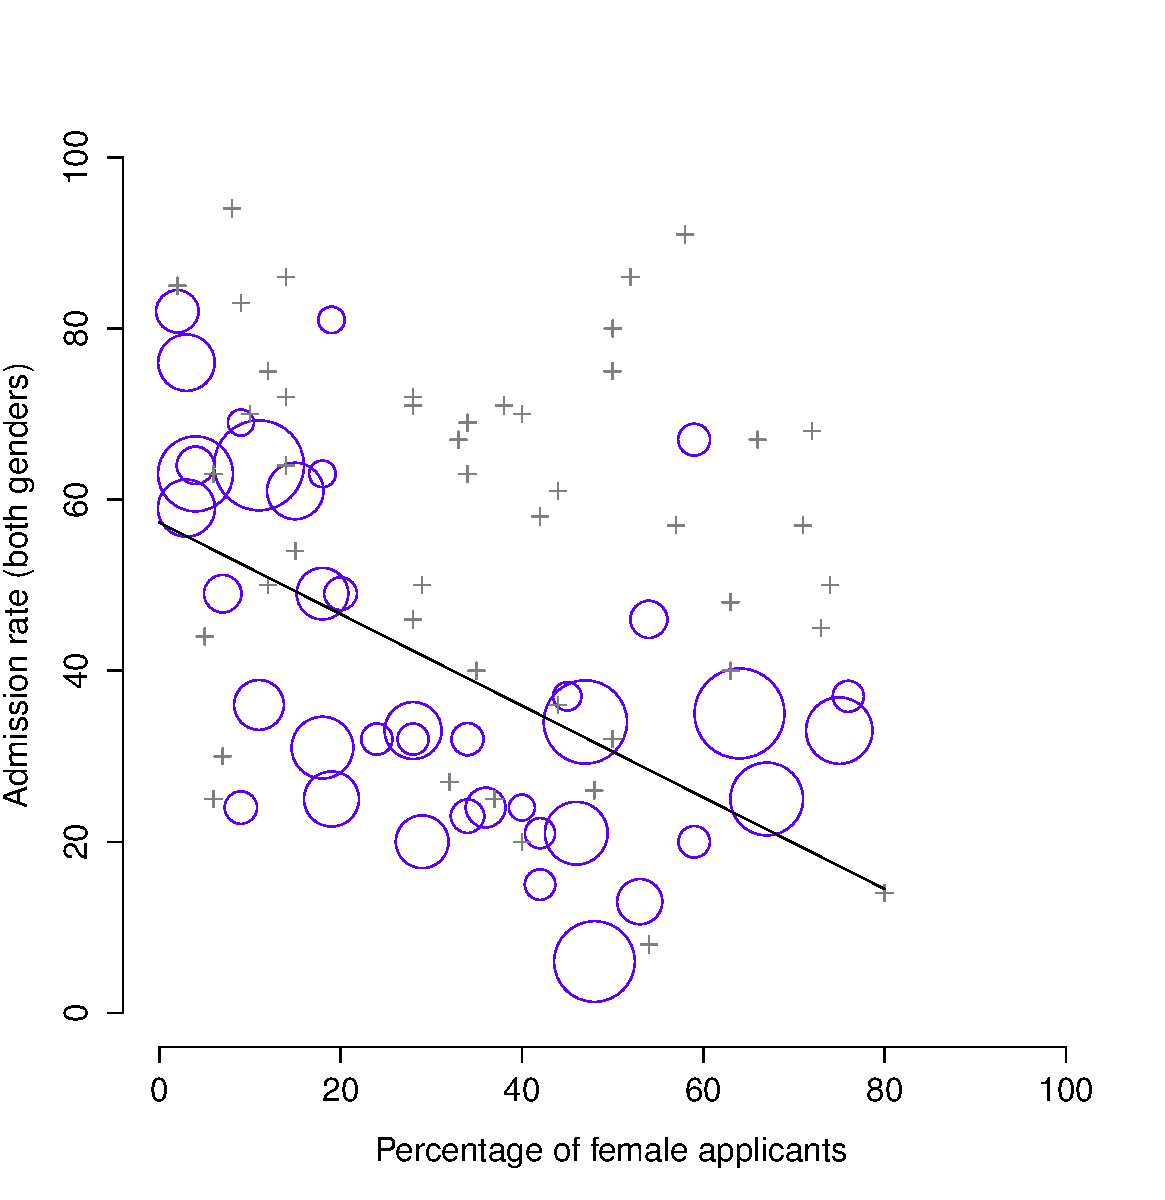
\includegraphics{img/whystats/berkeleyadmissions3-eps-converted-to.pdf}
\caption{\label{fig:berkeley}The Berkeley 1973 college admissions data. This figure plots the admission rate for the 85 departments that had at least one female applicant, as a function of the percentage of applicants that were female. The plot is a redrawing of Figure 1 from \citet{Bickel1975}. Circles plot departments with more than 40 applicants; the area of the circle is proportional to the total number of applicants. The crosses plot department with fewer than 40 applicants.}
\end{figure}

Before leaving this topic entirely, I want to point out something else really critical that is often overlooked in a research methods class. Statistics only solves \emph{part} of the problem. Remember that we started all this with the concern that Berkeley's admissions processes might be unfairly biased against female applicants. When we looked at the ``aggregated'' data, it did seem like the university was discriminating against women, but when we ``disaggregate'' and looked at the individual behaviour of all the departments, it turned out that the actual departments were, if anything, slightly biased in favour of women. The gender bias in total admissions was caused by the fact that women tended to self-select for harder departments. From a legal perspective, that would probably put the university in the clear. Postgraduate admissions are determined at the level of the individual department, and there are good reasons to do that. At the level of individual departments the decisions are more or less unbiased (the weak bias in favour of females at that level is small, and not consistent across departments). Since the university can't dictate which departments people choose to apply to, and the decision making takes place at the level of the department it can hardly be held accountable for any biases that those choices produce.

That was the basis for my somewhat glib remarks earlier, but that's not exactly the whole story, is it? After all, if we're interested in this from a more sociological and psychological perspective, we might want to ask \emph{why} there are such strong gender differences in applications. Why do males tend to apply to engineering more often than females, and why is this reversed for the English department? And why is it the case that the departments that tend to have a female-application bias tend to have lower overall admission rates than those departments that have a male-application bias? Might this not still reflect a gender bias, even though every single department is itself unbiased? It might. Suppose, hypothetically, that males preferred to apply to ``hard sciences'' and females prefer ``humanities''. And suppose further that the reason for why the humanities departments have low admission rates is because the government doesn't want to fund the humanities (Ph.D.~places, for instance, are often tied to government funded research projects). Does that constitute a gender bias? Or just an unenlightened view of the value of the humanities? What if someone at a high level in the government cut the humanities funds because they felt that the humanities are ``useless chick stuff''. That seems pretty \emph{blatantly} gender biased. None of this falls within the purview of statistics, but it matters to the research project. If you're interested in the overall structural effects of subtle gender biases, then you probably want to look at \emph{both} the aggregated and disaggregated data. If you're interested in the decision making process at Berkeley itself then you're probably only interested in the disaggregated data.

In short there are a lot of critical questions that you can't answer with statistics, but the answers to those questions will have a huge impact on how you analyse and interpret data. And this is the reason why you should always think of statistics as a \emph{tool} to help you learn about your data. No more and no less. It's a powerful tool to that end, but there's no substitute for careful thought.

\hypertarget{statistics-in-psychology}{%
\section{Statistics in psychology}\label{statistics-in-psychology}}

I hope that the discussion above helped explain why science in general is so focused on statistics. But I'm guessing that you have a lot more questions about what role statistics plays in psychology, and specifically why psychology classes always devote so many lectures to stats. So here's my attempt to answer a few of them\ldots{}

\textbf{Why does psychology have so much statistics?}

To be perfectly honest, there's a few different reasons, some of which are better than others. The most important reason is that psychology is a statistical science. What I mean by that is that the ``things'' that we study are \emph{people}. Real, complicated, gloriously messy, infuriatingly perverse people. The ``things'' of physics include objects like electrons, and while there are all sorts of complexities that arise in physics, electrons don't have minds of their own. They don't have opinions, they don't differ from each other in weird and arbitrary ways, they don't get bored in the middle of an experiment, and they don't get angry at the experimenter and then deliberately try to sabotage the data set (not that I've ever done that!). At a fundamental level psychology is harder than physics.\footnote{Which might explain why physics is just a teensy bit further advanced as a science than we are.}

Basically, we teach statistics to you as psychologists because you need to be better at stats than physicists. There's actually a saying used sometimes in physics, to the effect that ``if your experiment needs statistics, you should have done a better experiment''. They have the luxury of being able to say that because their objects of study are pathetically simple in comparison to the vast mess that confronts social scientists. And it's not just psychology. Most social sciences are desperately reliant on statistics. Not because we're bad experimenters, but because we've picked a harder problem to solve. We teach you stats because you really, really need it.

\textbf{Can't someone else do the statistics?}

To some extent, but not completely. It's true that you don't need to become a fully trained statistician just to do psychology, but you do need to reach a certain level of statistical competence. In my view, there's three reasons that every psychological researcher ought to be able to do basic statistics:

\begin{itemize}
\tightlist
\item
  Firstly, there's the fundamental reason: statistics is deeply intertwined with research design. If you want to be good at designing psychological studies, you need to at the very least understand the basics of stats.
\item
  Secondly, if you want to be good at the psychological side of the research, then you need to be able to understand the psychological literature, right? But almost every paper in the psychological literature reports the results of statistical analyses. So if you really want to understand the psychology, you need to be able to understand what other people did with their data. And that means understanding a certain amount of statistics.
\item
  Thirdly, there's a big practical problem with being dependent on other people to do all your statistics: statistical analysis is \emph{expensive}. If you ever get bored and want to look up how much the Australian government charges for university fees, you'll notice something interesting: statistics is designated as a ``national priority'' category, and so the fees are much, much lower than for any other area of study. This is because there's a massive shortage of statisticians out there. So, from your perspective as a psychological researcher, the laws of supply and demand aren't exactly on your side here! As a result, in almost any real life situation where you want to do psychological research, the cruel facts will be that you don't have enough money to afford a statistician. So the economics of the situation mean that you have to be pretty self-sufficient.
  Note that a lot of these reasons generalise beyond researchers. If you want to be a practicing psychologist and stay on top of the field, it helps to be able to read the scientific literature, which relies pretty heavily on statistics.
\end{itemize}

\textbf{I don't care about jobs, research, or clinical work. Do I need statistics?}

Okay, now you're just messing with me. Still, I think it should matter to you too. Statistics should matter to you in the same way that statistics should matter to \emph{everyone}. We live in the 21st century, and data are \emph{everywhere}. Frankly, given the world in which we live these days, a basic knowledge of statistics is pretty damn close to a survival tool! Which is the topic of the next section.

\hypertarget{statistics-in-everyday-life}{%
\section{Statistics in everyday life}\label{statistics-in-everyday-life}}

\begin{quote}
\emph{``We are drowning in information,~but we are starved for knowledge''}

-Various authors, original probably John Naisbitt
\end{quote}

When I started writing up my lecture notes I took the 20 most recent news articles posted to the ABC news website. Of those 20 articles, it turned out that 8 of them involved a discussion of something that I would call a statistical topic and 6 of those made a mistake. The most common error, if you're curious, was failing to report baseline data (e.g., the article mentions that 5\% of people in situation X have some characteristic Y, but doesn't say how common the characteristic is for everyone else!). The point I'm trying to make here isn't that journalists are bad at statistics (though they almost always are), it's that a basic knowledge of statistics is very helpful for trying to figure out when someone else is either making a mistake or even lying to you. In fact, one of the biggest things that a knowledge of statistics does to you is cause you to get angry at the newspaper or the internet on a far more frequent basis. You can find a good example of this in \ref{housingpriceexample}. In later versions of this book I'll try to include more anecdotes along those lines.

\hypertarget{theres-more-to-research-methods-than-statistics}{%
\section{There's more to research methods than statistics}\label{theres-more-to-research-methods-than-statistics}}

So far, most of what I've talked about is statistics, and so you'd be forgiven for thinking that statistics is all I care about in life. To be fair, you wouldn't be far wrong, but research methodology is a broader concept than statistics. So most research methods courses will cover a lot of topics that relate much more to the pragmatics of research design, and in particular the issues that you encounter when trying to do research with humans. However, about 99\% of student \emph{fears} relate to the statistics part of the course, so I've focused on the stats in this discussion, and hopefully I've convinced you that statistics matters, and more importantly, that it's not to be feared. That being said, it's pretty typical for introductory research methods classes to be very stats-heavy. This is not (usually) because the lecturers are evil people. Quite the contrary, in fact. Introductory classes focus a lot on the statistics because you almost always find yourself needing statistics before you need the other research methods training. Why? Because almost all of your assignments in other classes will rely on statistical training, to a much greater extent than they rely on other methodological tools. It's not common for undergraduate assignments to require you to design your own study from the ground up (in which case you would need to know a lot about research design), but it \emph{is} common for assignments to ask you to analyse and interpret data that were collected in a study that someone else designed (in which case you need statistics). In that sense, from the perspective of allowing you to do well in all your other classes, the statistics is more urgent.

But note that ``urgent'' is different from ``important'' -- they both matter. I really do want to stress that research design is just as important as data analysis, and this book does spend a fair amount of time on it. However, while statistics has a kind of universality, and provides a set of core tools that are useful for most types of psychological research, the research methods side isn't quite so universal. There are some general principles that everyone should think about, but a lot of research design is very idiosyncratic, and is specific to the area of research that you want to engage in. To the extent that it's the details that matter, those details don't usually show up in an introductory stats and research methods class.

\hypertarget{studydesign}{%
\chapter{A brief introduction to research design}\label{studydesign}}

\begin{quote}
\emph{To consult the statistician after an experiment is finished is often merely to ask him to conduct a post mortem examination. He can perhaps say what the experiment died of.}

-- Sir Ronald Fisher\footnote{Presidential Address to the First Indian Statistical Congress, 1938. Source: \url{http://en.wikiquote.org/wiki/Ronald_Fisher}}
\end{quote}

In this chapter, we're going to start thinking about the basic ideas that go into designing a study, collecting data, checking whether your data collection works, and so on. It won't give you enough information to allow you to design studies of your own, but it will give you a lot of the basic tools that you need to assess the studies done by other people. However, since the focus of this book is much more on data analysis than on data collection, I'm only giving a very brief overview. Note that this chapter is ``special'' in two ways. Firstly, it's much more psychology-specific than the later chapters. Secondly, it focuses much more heavily on the scientific problem of research methodology, and much less on the statistical problem of data analysis. Nevertheless, the two problems are related to one another, so it's traditional for stats textbooks to discuss the problem in a little detail. This chapter relies heavily on \citet{Campbell1963} for the discussion of study design, and \citet{Stevens1946} for the discussion of scales of measurement.

\hypertarget{measurement}{%
\section{Introduction to psychological measurement}\label{measurement}}

The first thing to understand is data collection can be thought of as a kind of \textbf{\emph{measurement}}. That is, what we're trying to do here is measure something about human behaviour or the human mind. What do I mean by ``measurement''?

\hypertarget{some-thoughts-about-psychological-measurement}{%
\subsection{Some thoughts about psychological measurement}\label{some-thoughts-about-psychological-measurement}}

Measurement itself is a subtle concept, but basically it comes down to finding some way of assigning numbers, or labels, or some other kind of well-defined descriptions, to ``stuff''. So, any of the following would count as a psychological measurement:

\begin{itemize}
\tightlist
\item
  My \textbf{age} is \emph{33 years}.
\item
  I \emph{do not} \textbf{like anchovies}.
\item
  My \textbf{chromosomal gender} is \emph{male}.
\item
  My \textbf{self-identified gender} is \emph{male}.\footnote{Well\ldots{} now this is awkward, isn't it? This section is one of the oldest parts of the book, and it's outdated in a rather embarrassing way. I wrote this in 2010, at which point all of those facts \emph{were} true. Revisiting this in 2018\ldots{} well I'm not 33 any more, but that's not surprising I suppose. I can't imagine my chromosomes have changed, so I'm going to guess my karyotype was then and is now XY. The self-identified gender, on the other hand\ldots{} ah. I suppose the fact that the title page now refers to me as Danielle rather than Daniel might possibly be a giveaway, but I don't typically identify as ``male'' on a gender questionnaire these days, and I prefer \emph{``she/her''} pronouns as a default (it's a long story)! I did think a little about how I was going to handle this in the book, actually. The book has a somewhat distinct authorial voice to it, and I feel like it would be a rather different work if I went back and wrote everything as Danielle and updated all the pronouns in the work. Besides, it would be a lot of work, so I've left my name as ``Dan'' throughout the book, and in ant case ``Dan'' is a perfectly good nickname for ``Danielle'', don't you think? In any case, it's not a big deal. I only wanted to mention it to make life a little easier for readers who aren't sure how to refer to me. I still don't like anchovies though :-)}
\end{itemize}

In the short list above, the \textbf{bolded part} is ``the thing to be measured'', and the \emph{italicised part} is ``the measurement itself''. In fact, we can expand on this a little bit, by thinking about the set of possible measurements that could have arisen in each case:

\begin{itemize}
\tightlist
\item
  My \textbf{age} (in years) could have been \emph{0, 1, 2, 3 \ldots{}}, etc. The upper bound on what my age could possibly be is a bit fuzzy, but in practice you'd be safe in saying that the largest possible age is \emph{150}, since no human has ever lived that long.
\item
  When asked if I \textbf{like anchovies}, I might have said that \emph{I do}, or \emph{I do not}, or \emph{I have no opinion}, or \emph{I sometimes do}.
\item
  My \textbf{chromosomal gender} is almost certainly going to be \emph{male (XY)} or \emph{female (XX)}, but there are a few other possibilities. I could also have \emph{Klinfelter's syndrome (XXY)}, which is more similar to male than to female. And I imagine there are other possibilities too.
\item
  My \textbf{self-identified gender} is also very likely to be \emph{male} or \emph{female}, but it doesn't have to agree with my chromosomal gender. I may also choose to identify with \emph{neither}, or to explicitly call myself \emph{transgender}.
\end{itemize}

As you can see, for some things (like age) it seems fairly obvious what the set of possible measurements should be, whereas for other things it gets a bit tricky. But I want to point out that even in the case of someone's age it's much more subtle than this. For instance, in the example above I assumed that it was okay to measure age in years. But if you're a developmental psychologist, that's way too crude, and so you often measure age in \emph{years and months} (if a child is 2 years and 11 months this is usually written as ``2;11''). If you're interested in newborns you might want to measure age in \emph{days since birth}, maybe even \emph{hours since birth}. In other words, the way in which you specify the allowable measurement values is important.

Looking at this a bit more closely, you might also realise that the concept of ``age'' isn't actually all that precise. In general, when we say ``age'' we implicitly mean ``the length of time since birth''. But that's not always the right way to do it. Suppose you're interested in how newborn babies control their eye movements. If you're interested in kids that young, you might also start to worry that ``birth'' is not the only meaningful point in time to care about. If Baby Alice is born 3 weeks premature and Baby Bianca is born 1 week late, would it really make sense to say that they are the ``same age'' if we encountered them ``2 hours after birth''? In one sense, yes. By social convention we use birth as our reference point for talking about age in everyday life, since it defines the amount of time the person has been operating as an independent entity in the world. But from a scientific perspective that's not the only thing we care about. When we think about the biology of human beings, it's often useful to think of ourselves as organisms that have been growing and maturing since conception, and from that perspective Alice and Bianca aren't the same age at all. So you might want to define the concept of ``age'' in two different ways: the length of time since conception and the length of time since birth. When dealing with adults it won't make much difference, but when dealing with newborns it might.

Moving beyond these issues, there's the question of methodology. What specific ``measurement method'' are you going to use to find out someone's age? As before, there are lots of different possibilities:

\begin{itemize}
\tightlist
\item
  You could just ask people ``how old are you?'' The method of self-report is fast, cheap and easy. But it only works with people old enough to understand the question, and some people lie about their age.
\item
  You could ask an authority (e.g., a parent) ``how old is your child?'' This method is fast, and when dealing with kids it's not all that hard since the parent is almost always around. It doesn't work as well if you want to know ``age since conception'', since a lot of parents can't say for sure when conception took place. For that, you might need a different authority (e.g., an obstetrician).
\item
  You could look up official records, for example birth or death certificates. This is a time consuming and frustrating endeavour, but it has its uses (e.g., if the person is now dead).
\end{itemize}

\hypertarget{operationalisation-defining-your-measurement}{%
\subsection{Operationalisation: defining your measurement}\label{operationalisation-defining-your-measurement}}

All of the ideas discussed in the previous section relate to the concept of \textbf{\emph{operationalisation}}. To be a bit more precise about the idea, operationalisation is the process by which we take a meaningful but somewhat vague concept and turn it into a precise measurement. The process of operationalisation can involve several different things:

\begin{itemize}
\tightlist
\item
  Being precise about what you are trying to measure. For instance, does ``age'' mean ``time since birth'' or ``time since conception'' in the context of your research?
\item
  Determining what method you will use to measure it. Will you use self-report to measure age, ask a parent, or look up an official record? If you're using self-report, how will you phrase the question?
\item
  Defining the set of allowable values that the measurement can take. Note that these values don't always have to be numerical, though they often are. When measuring age the values are numerical, but we still need to think carefully about what numbers are allowed. Do we want age in years, years and months, days, or hours? For other types of measurements (e.g., gender) the values aren't numerical. But, just as before, we need to think about what values are allowed. If we're asking people to self-report their gender, what options to we allow them to choose between? Is it enough to allow only ``male'' or ``female''? Do you need an ``other'' option? Or should we not give people specific options and instead let them answer in their own words? And if you open up the set of possible values to include all verbal response, how will you interpret their answers?
\end{itemize}

Operationalisation is a tricky business, and there's no ``one, true way'' to do it. The way in which you choose to operationalise the informal concept of ``age'' or ``gender'' into a formal measurement depends on what you need to use the measurement for. Often you'll find that the community of scientists who work in your area have some fairly well-established ideas for how to go about it. In other words, operationalisation needs to be thought through on a case by case basis. Nevertheless, while there a lot of issues that are specific to each individual research project, there are some aspects to it that are pretty general.

Before moving on I want to take a moment to clear up our terminology, and in the process introduce one more term. Here are four different things that are closely related to each other:

\begin{itemize}
\tightlist
\item
  \textbf{\emph{A theoretical construct}}. This is the thing that you're trying to take a measurement of, like ``age'', ``gender'' or an ``opinion''. A theoretical construct can't be directly observed, and often they're actually a bit vague.
\item
  \textbf{\emph{A measure}}. The measure refers to the method or the tool that you use to make your observations. A question in a survey, a behavioural observation or a brain scan could all count as a measure.
\item
  \textbf{\emph{An operationalisation}}. The term ``operationalisation'' refers to the logical connection between the measure and the theoretical construct, or to the process by which we try to derive a measure from a theoretical construct.
\item
  \textbf{\emph{A variable}}. Finally, a new term. A variable is what we end up with when we apply our measure to something in the world. That is, variables are the actual ``data'' that we end up with in our data sets.
\end{itemize}

In practice, even scientists tend to blur the distinction between these things, but it's very helpful to try to understand the differences.

\hypertarget{scales}{%
\section{Scales of measurement}\label{scales}}

As the previous section indicates, the outcome of a psychological measurement is called a variable. But not all variables are of the same qualitative type and so it's useful to understand what types there are. A very useful concept for distinguishing between different types of variables is what's known as \textbf{\emph{scales of measurement}}.

\hypertarget{nominal-scale}{%
\subsection{Nominal scale}\label{nominal-scale}}

A \textbf{\emph{nominal scale}} variable (also referred to as a \textbf{\emph{categorical}} variable) is one in which there is no particular relationship between the different possibilities. For these kinds of variables it doesn't make any sense to say that one of them is ``bigger' or''better" than any other one, and it absolutely doesn't make any sense to average them. The classic example for this is ``eye colour''. Eyes can be blue, green or brown, amongst other possibilities, but none of them is any ``bigger'' than any other one. As a result, it would feel really weird to talk about an ``average eye colour''. Similarly, gender is nominal too: male isn't better or worse than female. Neither does it make sense to try to talk about an ``average gender''. In short, nominal scale variables are those for which the only thing you can say about the different possibilities is that they are different. That's it.

Let's take a slightly closer look at this. Suppose I was doing research on how people commute to and from work. One variable I would have to measure would be what kind of transportation people use to get to work. This ``transport type'' variable could have quite a few possible values, including: ``train'', ``bus'', ``car'', ``bicycle''. For now, let's suppose that these four are the only possibilities. Then imagine that I ask 100 people how they got to work today, with this result:

\begin{longtable}[]{@{}cc@{}}
\toprule
Transportation & Number of people \\
\midrule
\endhead
(1) Train & 12 \\
(2) Bus & 30 \\
(3) Car & 48 \\
(4) Bicycle & 10 \\
\bottomrule
\end{longtable}

So, what's the average transportation type? Obviously, the answer here is that there isn't one. It's a silly question to ask. You can say that travel by car is the most popular method, and travel by train is the least popular method, but that's about all. Similarly, notice that the order in which I list the options isn't very interesting. I could have chosen to display the data like this

\begin{longtable}[]{@{}cc@{}}
\toprule
Transportation & Number of people \\
\midrule
\endhead
(3) Car & 48 \\
(1) Train & 12 \\
(4) Bicycle & 10 \\
(2) Bus & 30 \\
\bottomrule
\end{longtable}

and nothing really changes.

\hypertarget{ordinal-scale}{%
\subsection{Ordinal scale}\label{ordinal-scale}}

\textbf{\emph{Ordinal scale}} variables have a bit more structure than nominal scale variables, but not by a lot. An ordinal scale variable is one in which there is a natural, meaningful way to order the different possibilities, but you can't do anything else. The usual example given of an ordinal variable is ``finishing position in a race''. You \emph{can} say that the person who finished first was faster than the person who finished second, but you \emph{don't} know how much faster. As a consequence we know that 1st \(>\) 2nd, and we know that 2nd \(>\) 3rd, but the difference between 1st and 2nd might be much larger than the difference between 2nd and 3rd.

Here's a more psychologically interesting example. Suppose I'm interested in people's attitudes to climate change. I then go and ask some people to pick the statement (from four listed statements) that most closely matches their beliefs:

\begin{itemize}
\item
  \begin{enumerate}
  \def\labelenumi{(\arabic{enumi})}
  \tightlist
  \item
    Temperatures are rising because of human activity
  \end{enumerate}
\item
  \begin{enumerate}
  \def\labelenumi{(\arabic{enumi})}
  \setcounter{enumi}{1}
  \tightlist
  \item
    Temperatures are rising but we don't know why
  \end{enumerate}
\item
  \begin{enumerate}
  \def\labelenumi{(\arabic{enumi})}
  \setcounter{enumi}{2}
  \tightlist
  \item
    Temperatures are rising but not because of humans
  \end{enumerate}
\item
  \begin{enumerate}
  \def\labelenumi{(\arabic{enumi})}
  \setcounter{enumi}{3}
  \tightlist
  \item
    Temperatures are not rising
  \end{enumerate}
\end{itemize}

Notice that these four statements actually do have a natural ordering, in terms of ``the extent to which they agree with the current science''. Statement 1 is a close match, statement 2 is a reasonable match, statement 3 isn't a very good match, and statement 4 is in strong opposition to current science. So, in terms of the thing I'm interested in (the extent to which people endorse the science), I can order the items as \(1 > 2 > 3 > 4\). Since this ordering exists, it would be very weird to list the options like this

\begin{itemize}
\item
  \begin{enumerate}
  \def\labelenumi{(\arabic{enumi})}
  \setcounter{enumi}{2}
  \tightlist
  \item
    Temperatures are rising but not because of humans
  \end{enumerate}
\item
  \begin{enumerate}
  \def\labelenumi{(\arabic{enumi})}
  \tightlist
  \item
    Temperatures are rising because of human activity
  \end{enumerate}
\item
  \begin{enumerate}
  \def\labelenumi{(\arabic{enumi})}
  \setcounter{enumi}{3}
  \tightlist
  \item
    Temperatures are not rising
  \end{enumerate}
\item
  \begin{enumerate}
  \def\labelenumi{(\arabic{enumi})}
  \setcounter{enumi}{1}
  \tightlist
  \item
    Temperatures are rising but we don't know why
  \end{enumerate}
\end{itemize}

because it seems to violate the natural ``structure'' to the question.

So, let's suppose I asked 100 people these questions, and got the following answers

\begin{longtable}[]{@{}lc@{}}
\toprule
Response & Number \\
\midrule
\endhead
(1) Temperatures are rising, because of human activity & 51 \\
(2) Temperatures are rising, but we don't know why & 20 \\
(3) Temperatures are rising, but not because of humans & 10 \\
(4) Temperatures are not rising & 19 \\
\bottomrule
\end{longtable}

When analysing these data it seems quite reasonable to try to group (1), (2) and (3) together, and say that 81 out of 100 people were willing to \emph{at least partially} endorse the science. And it's \emph{also} quite reasonable to group (2), (3) and (4) together and say that 49 out of 100 people registered \emph{at least some disagreement} with the dominant scientific view. However, it would be entirely bizarre to try to group (1), (2) and (4) together and say that 90 out of 100 people said \ldots{} what? There's nothing sensible that allows you to group those responses together at all.

That said, notice that while we \emph{can} use the natural ordering of these items to construct sensible groupings, what we \emph{can't} do is average them. For instance, in my simple example here, the ``average'' response to the question is 1.97. If you can tell me what that means I'd love to know, because it seems like gibberish to me!

\hypertarget{interval-scale}{%
\subsection{Interval scale}\label{interval-scale}}

In contrast to nominal and ordinal scale variables, \textbf{\emph{interval scale}} and ratio scale variables are variables for which the numerical value is genuinely meaningful. In the case of interval scale variables the \emph{differences} between the numbers are interpretable, but the variable doesn't have a ``natural'' zero value. A good example of an interval scale variable is measuring temperature in degrees celsius. For instance, if it was 15\(^\circ\) yesterday and 18\(^\circ\) today, then the 3\(^\circ\) difference between the two is genuinely meaningful. Moreover, that 3\(^\circ\) difference is \emph{exactly the same} as the 3\(^\circ\) difference between \(7^\circ\) and \(10^\circ\). In short, addition and subtraction are meaningful for interval scale variables.\footnote{Actually, I've been informed by readers with greater physics knowledge than I that temperature isn't strictly an interval scale, in the sense that the amount of energy required to heat something up by 3\(^\circ\) depends on it's current temperature. So in the sense that physicists care about, temperature isn't actually an interval scale. But it still makes a cute example so I'm going to ignore this little inconvenient truth.}

However, notice that the \(0^\circ\) does not mean ``no temperature at all''. It actually means ``the temperature at which water freezes'', which is pretty arbitrary. As a consequence it becomes pointless to try to multiply and divide temperatures. It is wrong to say that \(20^\circ\) is \emph{twice as hot} as \(10^\circ\), just as it is weird and meaningless to try to claim that \(20^\circ\) is negative two times as hot as \(-10^\circ\).

Again, lets look at a more psychological example. Suppose I'm interested in looking at how the attitudes of first-year university students have changed over time. Obviously, I'm going to want to record the year in which each student started. This is an interval scale variable. A student who started in 2003 did arrive 5 years before a student who started in 2008. However, it would be completely daft for me to divide 2008 by 2003 and say that the second student started ``1.0024 times later'' than the first one. That doesn't make any sense at all.

\hypertarget{ratio-scale}{%
\subsection{Ratio scale}\label{ratio-scale}}

The fourth and final type of variable to consider is a \textbf{\emph{ratio scale}} variable, in which zero really means zero, and it's okay to multiply and divide. A good psychological example of a ratio scale variable is response time (RT). In a lot of tasks it's very common to record the amount of time somebody takes to solve a problem or answer a question, because it's an indicator of how difficult the task is. Suppose that Alan takes 2.3 seconds to respond to a question, whereas Ben takes 3.1 seconds. As with an interval scale variable, addition and subtraction are both meaningful here. Ben really did take \(3.1 - 2.3 = 0.8\) seconds longer than Alan did. However, notice that multiplication and division also make sense here too: Ben took \(3.1 / 2.3 = 1.35\) times as long as Alan did to answer the question. And the reason why you can do this is that for a ratio scale variable such as RT ``zero seconds'' really does mean ``no time at all''.

\hypertarget{continuousdiscrete}{%
\subsection{Continuous versus discrete variables}\label{continuousdiscrete}}

There's a second kind of distinction that you need to be aware of, regarding what types of variables you can run into. This is the distinction between continuous variables and discrete variables. The difference between these is as follows:

\begin{itemize}
\tightlist
\item
  A \textbf{\emph{continuous variable}} is one in which, for any two values that you can think of, it's always logically possible to have another value in between.
\item
  A \textbf{\emph{discrete variable}} is, in effect, a variable that isn't continuous. For a discrete variable it's sometimes the case that there's nothing in the middle.
\end{itemize}

These definitions probably seem a bit abstract, but they're pretty simple once you see some examples. For instance, response time is continuous. If Alan takes 3.1 seconds and Ben takes 2.3 seconds to respond to a question, then Cameron's response time will lie in between if he took 3.0 seconds. And of course it would also be possible for David to take 3.031 seconds to respond, meaning that his RT would lie in between Cameron's and Alan's. And while in practice it might be impossible to measure RT that precisely, it's certainly possible in principle. Because we can always find a new value for RT in between any two other ones we regard RT as a continuous measure.

Discrete variables occur when this rule is violated. For example, nominal scale variables are always discrete. There isn't a type of transportation that falls ``in between'' trains and bicycles, not in the strict mathematical way that 2.3 falls in between 2 and 3. So transportation type is discrete. Similarly, ordinal scale variables are always discrete. Although ``2nd place'' does fall between ``1st place'' and ``3rd place'', there's nothing that can logically fall in between ``1st place'' and ``2nd place''. Interval scale and ratio scale variables can go either way. As we saw above, response time (a ratio scale variable) is continuous. Temperature in degrees celsius (an interval scale variable) is also continuous. However, the year you went to school (an interval scale variable) is discrete. There's no year in between 2002 and 2003. The number of questions you get right on a true-or-false test (a ratio scale variable) is also discrete. Since a true-or-false question doesn't allow you to be ``partially correct'', there's nothing in between 5/10 and 6/10. Table \ref{tab:scalescont} summarises the relationship between the scales of measurement and the discrete/continuity distinction. Cells with a tick mark correspond to things that are possible. I'm trying to hammer this point home, because (a) some textbooks get this wrong, and (b) people very often say things like ``discrete variable'' when they mean ``nominal scale variable''. It's very unfortunate.

\begin{table}

\caption{\label{tab:scalescont}The relationship between the scales of measurement and the discrete/continuity distinction. Cells with a tick mark correspond to things that are possible.}
\centering
\begin{tabular}[t]{lcc}
\toprule
 & continuous & discrete\\
\midrule
nominal &  & \$\textbackslash{}checkmark\$\\
ordinal &  & \$\textbackslash{}checkmark\$\\
interval & \$\textbackslash{}checkmark\$ & \$\textbackslash{}checkmark\$\\
ratio & \$\textbackslash{}checkmark\$ & \$\textbackslash{}checkmark\$\\
\bottomrule
\end{tabular}
\end{table}

\hypertarget{some-complexities}{%
\subsection{Some complexities}\label{some-complexities}}

Okay, I know you're going to be shocked to hear this, but the real world is much messier than this little classification scheme suggests. Very few variables in real life actually fall into these nice neat categories, so you need to be kind of careful not to treat the scales of measurement as if they were hard and fast rules. It doesn't work like that. They're guidelines, intended to help you think about the situations in which you should treat different variables differently. Nothing more.

So let's take a classic example, maybe \emph{the} classic example, of a psychological measurement tool: the \textbf{\emph{Likert scale}}. The humble Likert scale is the bread and butter tool of all survey design. You yourself have filled out hundreds, maybe thousands, of them and odds are you've even used one yourself. Suppose we have a survey question that looks like this:

\begin{quote}
Which of the following best describes your opinion of the statement that ``all pirates are freaking awesome''?
\end{quote}

and then the options presented to the participant are these:

\begin{enumerate}
\def\labelenumi{(\arabic{enumi})}
\tightlist
\item
  Strongly disagree
\item
  Disagree
\item
  Neither agree nor disagree
\item
  Agree
\item
  Strongly agree
\end{enumerate}

This set of items is an example of a 5-point Likert scale, in which people are asked to choose among one of several (in this case 5) clearly ordered possibilities, generally with a verbal descriptor given in each case. However, it's not necessary that all items are explicitly described. This is a perfectly good example of a 5-point Likert scale too:

\begin{enumerate}
\def\labelenumi{(\arabic{enumi})}
\tightlist
\item
  Strongly disagree
\item
\item
\item
\item
  Strongly agree
\end{enumerate}

Likert scales are very handy, if somewhat limited, tools. The question is what kind of variable are they? They're obviously discrete, since you can't give a response of 2.5. They're obviously not nominal scale, since the items are ordered; and they're not ratio scale either, since there's no natural zero.

But are they ordinal scale or interval scale? One argument says that we can't really prove that the difference between ``strongly agree'' and ``agree'' is of the same size as the difference between ``agree'' and ``neither agree nor disagree''. In fact, in everyday life it's pretty obvious that they're not the same at all. So this suggests that we ought to treat Likert scales as ordinal variables. On the other hand, in practice most participants do seem to take the whole ``on a scale from 1 to 5'' part fairly seriously, and they tend to act as if the differences between the five response options were fairly similar to one another. As a consequence, a lot of researchers treat Likert scale data as interval scale.\footnote{Ah, psychology \ldots{} never an easy answer to anything!} It's not interval scale, but in practice it's close enough that we usually think of it as being \textbf{\emph{quasi-interval scale}}.

\hypertarget{reliability}{%
\section{Assessing the reliability of a measurement}\label{reliability}}

At this point we've thought a little bit about how to operationalise a theoretical construct and thereby create a psychological measure. And we've seen that by applying psychological measures we end up with variables, which can come in many different types. At this point, we should start discussing the obvious question: is the measurement any good? We'll do this in terms of two related ideas: \emph{reliability} and \emph{validity}. Put simply, the \textbf{\emph{reliability}} of a measure tells you how \emph{precisely} you are measuring something, whereas the validity of a measure tells you how \emph{accurate} the measure is. In this section I'll talk about reliability; we'll talk about validity in section \ref{validity}.

Reliability is actually a very simple concept. It refers to the repeatability or consistency of your measurement. The measurement of my weight by means of a ``bathroom scale'' is very reliable. If I step on and off the scales over and over again, it'll keep giving me the same answer. Measuring my intelligence by means of ``asking my mum'' is very unreliable. Some days she tells me I'm a bit thick, and other days she tells me I'm a complete idiot. Notice that this concept of reliability is different to the question of whether the measurements are correct (the correctness of a measurement relates to it's validity). If I'm holding a sack of potatos when I step on and off the bathroom scales the measurement will still be reliable: it will always give me the same answer. However, this highly reliable answer doesn't match up to my true weight at all, therefore it's wrong. In technical terms, this is a \emph{reliable but invalid} measurement. Similarly, whilst my mum's estimate of my intelligence is a bit unreliable, she might be right. Maybe I'm just not too bright, and so while her estimate of my intelligence fluctuates pretty wildly from day to day, it's basically right. That would be an \emph{unreliable but valid} measure. Of course, if my mum's estimates are too unreliable it's going to be very hard to figure out which one of her many claims about my intelligence is actually the right one. To some extent, then, a very unreliable measure tends to end up being invalid for practical purposes; so much so that many people would say that reliability is necessary (but not sufficient) to ensure validity.

Okay, now that we're clear on the distinction between reliability and validity, let's have a think about the different ways in which we might measure reliability:

\begin{itemize}
\tightlist
\item
  \textbf{\emph{Test-retest reliability}}. This relates to consistency over time. If we repeat the measurement at a later date do we get a the same answer?
\item
  \textbf{\emph{Inter-rater reliability}}. This relates to consistency across people. If someone else repeats the measurement (e.g., someone else rates my intelligence) will they produce the same answer?
\item
  \textbf{\emph{Parallel forms reliability}}. This relates to consistency across theoretically-equivalent measurements. If I use a different set of bathroom scales to measure my weight does it give the same answer?
\item
  \textbf{\emph{Internal consistency reliability}}. If a measurement is constructed from lots of different parts that perform similar functions (e.g., a personality questionnaire result is added up across several questions) do the individual parts tend to give similar answers. We'll look at this particular form of reliability later in the book, in Section \ref{rel}.
\end{itemize}

Not all measurements need to possess all forms of reliability. For instance, educational assessment can be thought of as a form of measurement. One of the subjects that I teach, \emph{Computational Cognitive Science}, has an assessment structure that has a research component and an exam component (plus other things). The exam component is \emph{intended} to measure something different from the research component, so the assessment as a whole has low internal consistency. However, within the exam there are several questions that are intended to (approximately) measure the same things, and those tend to produce similar outcomes. So the exam on its own has a fairly high internal consistency. Which is as it should be. You should only demand reliability in those situations where you want to be measuring the same thing!

\hypertarget{ivdv}{%
\section{The ``role'' of variables: predictors and outcomes}\label{ivdv}}

I've got one last piece of terminology that I need to explain to you before moving away from variables. Normally, when we do some research we end up with lots of different variables. Then, when we analyse our data, we usually try to explain some of the variables in terms of some of the other variables. It's important to keep the two roles ``thing doing the explaining'' and ``thing being explained'' distinct. So let's be clear about this now. First, we might as well get used to the idea of using mathematical symbols to describe variables, since it's going to happen over and over again. Let's denote the ``to be explained'' variable \(Y\), and denote the variables ``doing the explaining'' as \(X_1\), \(X_2\), etc.

When we are doing an analysis we have different names for \(X\) and \(Y\), since they play different roles in the analysis. The classical names for these roles are \textbf{\emph{independent variable}} (IV) and \textbf{\emph{dependent variable}} (DV). The IV is the variable that you use to do the explaining (i.e., \(X\)) and the DV is the variable being explained (i.e., \(Y\)). The logic behind these names goes like this: if there really is a relationship between \(X\) and \(Y\) then we can say that \(Y\) depends on \(X\), and if we have designed our study ``properly'' then \(X\) isn't dependent on anything else. However, I personally find those names horrible. They're hard to remember and they're highly misleading because (a) the IV is never actually ``independent of everything else'', and (b) if there's no relationship then the DV doesn't actually depend on the IV. And in fact, because I'm not the only person who thinks that IV and DV are just awful names, there are a number of alternatives that I find more appealing. The terms that I'll use in this book are \textbf{\emph{predictors}} and \textbf{\emph{outcomes}}. The idea here is that what you're trying to do is use \(X\) (the predictors) to make guesses about \(Y\) (the outcomes).\footnote{Annoyingly though, there's a lot of different names used out there. I won't list all of them -- there would be no point in doing that -- other than to note that ``response variable'' is sometimes used where I've used ``outcome''. Sigh. This sort of terminological confusion is very common, I'm afraid.} This is summarised in Table \ref{tab:ivdv}.

\begin{table}

\caption{\label{tab:ivdv}The terminology used to distinguish between different roles that a variable can play when analysing a data set. Note that this book will tend to avoid the classical terminology in favour of the newer names.}
\centering
\begin{tabular}[t]{lll}
\toprule
role of the variable & classical name & modern name\\
\midrule
to be explained & dependent variable (DV) & outcome\\
to do the explaining & independent variable (IV) & predictor\\
\bottomrule
\end{tabular}
\end{table}

\hypertarget{researchdesigns}{%
\section{Experimental and non-experimental research}\label{researchdesigns}}

One of the big distinctions that you should be aware of is the distinction between ``experimental research'' and ``non-experimental research''. When we make this distinction, what we're really talking about is the degree of control that the researcher exercises over the people and events in the study.

\hypertarget{experimental-research}{%
\subsection{Experimental research}\label{experimental-research}}

The key feature of \textbf{\emph{experimental research}} is that the researcher controls all aspects of the study, especially what participants experience during the study. In particular, the researcher manipulates or varies the predictor variables (IVs) but allows the outcome variable (DV) to vary naturally. The idea here is to deliberately vary the predictors (IVs) to see if they have any causal effects on the outcomes. Moreover, in order to ensure that there's no possibility that something other than the predictor variables is causing the outcomes, everything else is kept constant or is in some other way ``balanced'', to ensure that they have no effect on the results. In practice, it's almost impossible to \emph{think} of everything else that might have an influence on the outcome of an experiment, much less keep it constant. The standard solution to this is \textbf{\emph{randomisation}}. That is, we randomly assign people to different groups, and then give each group a different treatment (i.e., assign them different values of the predictor variables). We'll talk more about randomisation later, but for now it's enough to say that what randomisation does is minimise (but not eliminate) the possibility that there are any systematic difference between groups.

Let's consider a very simple, completely unrealistic and grossly unethical example. Suppose you wanted to find out if smoking causes lung cancer. One way to do this would be to find people who smoke and people who don't smoke and look to see if smokers have a higher rate of lung cancer. This is \emph{not} a proper experiment, since the researcher doesn't have a lot of control over who is and isn't a smoker. And this really matters. For instance, it might be that people who choose to smoke cigarettes also tend to have poor diets, or maybe they tend to work in asbestos mines, or whatever. The point here is that the groups (smokers and non-smokers) actually differ on lots of things, not \emph{just} smoking. So it might be that the higher incidence of lung cancer among smokers is caused by something else, and not by smoking per se. In technical terms these other things (e.g.~diet) are called ``confounders'', and we'll talk about those in just a moment.

In the meantime, let's consider what a proper experiment might look like. Recall that our concern was that smokers and non-smokers might differ in lots of ways. The solution, as long as you have no ethics, is to \emph{control} who smokes and who doesn't. Specifically, if we randomly divide young non-smokers into two groups and force half of them to become smokers, then it's very unlikely that the groups will differ in any respect other than the fact that half of them smoke. That way, if our smoking group gets cancer at a higher rate than the non-smoking group, we can feel pretty confident that (a) smoking does cause cancer and (b) we're murderers.

\hypertarget{non-experimental-research}{%
\subsection{Non-experimental research}\label{non-experimental-research}}

\textbf{\emph{Non-experimental research}} is a broad term that covers ``any study in which the researcher doesn't have as much control as they do in an experiment''. Obviously, control is something that scientists like to have, but as the previous example illustrates there are lots of situations in which you can't or shouldn't try to obtain that control. Since it's grossly unethical (and almost certainly criminal) to force people to smoke in order to find out if they get cancer, this is a good example of a situation in which you really shouldn't try to obtain experimental control. But there are other reasons too. Even leaving aside the ethical issues, our ``smoking experiment'' does have a few other issues. For instance, when I suggested that we ``force'' half of the people to become smokers, I was talking about \emph{starting} with a sample of non-smokers, and then forcing them to become smokers. While this sounds like the kind of solid, evil experimental design that a mad scientist would love, it might not be a very sound way of investigating the effect in the real world. For instance, suppose that smoking only causes lung cancer when people have poor diets, and suppose also that people who normally smoke do tend to have poor diets. However, since the ``smokers'' in our experiment aren't ``natural'' smokers (i.e., we forced non-smokers to become smokers, but they didn't take on all of the other normal, real life characteristics that smokers might tend to possess) they probably have better diets. As such, in this silly example they wouldn't get lung cancer and our experiment will fail, because it violates the structure of the ``natural'' world (the technical name for this is an ``artefactual'' result).

One distinction worth making between two types of non-experimental research is the difference between \textbf{\emph{quasi-experimental research}} and \textbf{\emph{case studies}}. The example I discussed earlier, in which we wanted to examine incidence of lung cancer among smokers and non-smokers without trying to control who smokes and who doesn't, is a quasi-experimental design. That is, it's the same as an experiment but we don't control the predictors (IVs). We can still use statistics to analyse the results, but we have to be a lot more careful and circumspect.

The alternative approach, case studies, aims to provide a very detailed description of one or a few instances. In general, you can't use statistics to analyse the results of case studies and it's usually very hard to draw any general conclusions about ``people in general'' from a few isolated examples. However, case studies are very useful in some situations. Firstly, there are situations where you don't have any alternative. Neuropsychology has this issue a lot. Sometimes, you just can't find a lot of people with brain damage in a specific brain area, so the only thing you can do is describe those cases that you do have in as much detail and with as much care as you can. However, there's also some genuine advantages to case studies. Because you don't have as many people to study you have the ability to invest lots of time and effort trying to understand the specific factors at play in each case. This is a very valuable thing to do. As a consequence, case studies can complement the more statistically-oriented approaches that you see in experimental and quasi-experimental designs. We won't talk much about case studies in this book, but they are nevertheless very valuable tools!

\hypertarget{validity}{%
\section{Assessing the validity of a study}\label{validity}}

More than any other thing, a scientist wants their research to be ``valid''. The conceptual idea behind \textbf{\emph{validity}} is very simple. Can you trust the results of your study? If not, the study is invalid. However, whilst it's easy to state, in practice it's much harder to check validity than it is to check reliability. And in all honesty, there's no precise, clearly agreed upon notion of what validity actually is. In fact, there are lots of different kinds of validity, each of which raises it's own issues. And not all forms of validity are relevant to all studies. I'm going to talk about five different types of validity:

\begin{itemize}
\tightlist
\item
  Internal validity
\item
  External validity
\item
  Construct validity
\item
  Face validity
\item
  Ecological validity
\end{itemize}

First, a quick guide as to what matters here. (1) Internal and external validity are the most important, since they tie directly to the fundamental question of whether your study really works. (2) Construct validity asks whether you're measuring what you think you are. (3) Face validity isn't terribly important except insofar as you care about ``appearances''. (4) Ecological validity is a special case of face validity that corresponds to a kind of appearance that you might care about a lot.

\hypertarget{internal-validity}{%
\subsection{Internal validity}\label{internal-validity}}

\textbf{\emph{Internal validity}} refers to the extent to which you are able draw the correct conclusions about the causal relationships between variables. It's called ``internal'' because it refers to the relationships between things ``inside'' the study. Let's illustrate the concept with a simple example. Suppose you're interested in finding out whether a university education makes you write better. To do so, you get a group of first year students, ask them to write a 1000 word essay, and count the number of spelling and grammatical errors they make. Then you find some third-year students, who obviously have had more of a university education than the first-years, and repeat the exercise. And let's suppose it turns out that the third-year students produce fewer errors. And so you conclude that a university education improves writing skills. Right? Except that the big problem with this experiment is that the third-year students are older and they've had more experience with writing things. So it's hard to know for sure what the causal relationship is. Do older people write better? Or people who have had more writing experience? Or people who have had more education? Which of the above is the true \emph{cause} of the superior performance of the third-years? Age? Experience? Education? You can't tell. This is an example of a failure of internal validity, because your study doesn't properly tease apart the \emph{causal} relationships between the different variables.

\hypertarget{external-validity}{%
\subsection{External validity}\label{external-validity}}

\textbf{\emph{External validity}} relates to the \textbf{\emph{generalisability}} or \textbf{\emph{applicability}} of your findings. That is, to what extent do you expect to see the same pattern of results in ``real life'' as you saw in your study. To put it a bit more precisely, any study that you do in psychology will involve a fairly specific set of questions or tasks, will occur in a specific environment, and will involve participants that are drawn from a particular subgroup (disappointingly often it is college students!). So, if it turns out that the results don't actually generalise or apply to people and situations beyond the ones that you studied, then what you've got is a lack of external validity.

The classic example of this issue is the fact that a very large proportion of studies in psychology will use undergraduate psychology students as the participants. Obviously, however, the researchers don't care \emph{only} about psychology students. They care about people in general. Given that, a study that uses only psychology students as participants always carries a risk of lacking external validity. That is, if there's something ``special'' about psychology students that makes them different to the general population in some \emph{relevant} respect, then we may start worrying about a lack of external validity.

That said, it is absolutely critical to realise that a study that uses only psychology students does not necessarily have a problem with external validity. I'll talk about this again later, but it's such a common mistake that I'm going to mention it here. The external validity of a study is threatened by the choice of population if (a) the population from which you sample your participants is very narrow (e.g., psychology students), and (b) the narrow population that you sampled from is systematically different from the general population \emph{in some respect that is relevant to the psychological phenomenon that you intend to study}. The italicised part is the bit that lots of people forget. It is true that psychology undergraduates differ from the general population in lots of ways, and so a study that uses only psychology students \emph{may} have problems with external validity. However, if those differences aren't very relevant to the phenomenon that you're studying, then there's nothing to worry about. To make this a bit more concrete here are two extreme examples:

\begin{itemize}
\tightlist
\item
  You want to measure ``attitudes of the general public towards psychotherapy'', but all of your participants are psychology students. This study would almost certainly have a problem with external validity.
\item
  You want to measure the effectiveness of a visual illusion, and your participants are all psychology students. This study is unlikely to have a problem with external validity
\end{itemize}

Having just spent the last couple of paragraphs focusing on the choice of participants, since that's a big issue that everyone tends to worry most about, it's worth remembering that external validity is a broader concept. The following are also examples of things that might pose a threat to external validity, depending on what kind of study you're doing:

\begin{itemize}
\tightlist
\item
  People might answer a ``psychology questionnaire'' in a manner that doesn't reflect what they would do in real life.
\item
  Your lab experiment on (say) ``human learning'' has a different structure to the learning problems people face in real life.
\end{itemize}

\hypertarget{construct-validity}{%
\subsection{Construct validity}\label{construct-validity}}

\textbf{\emph{Construct validity}} is basically a question of whether you're measuring what you want to be measuring. A measurement has good construct validity if it is actually measuring the correct theoretical construct, and bad construct validity if it doesn't. To give a very simple (if ridiculous) example, suppose I'm trying to investigate the rates with which university students cheat on their exams. And the way I attempt to measure it is by asking the cheating students to stand up in the lecture theatre so that I can count them. When I do this with a class of 300 students 0 people claim to be cheaters. So I therefore conclude that the proportion of cheaters in my class is 0\%. Clearly this is a bit ridiculous. But the point here is not that this is a very deep methodological example, but rather to explain what construct validity is. The problem with my measure is that while I'm \emph{trying} to measure ``the proportion of people who cheat'' what I'm actually measuring is ``the proportion of people stupid enough to own up to cheating, or bloody minded enough to pretend that they do''. Obviously, these aren't the same thing! So my study has gone wrong, because my measurement has very poor construct validity.

\hypertarget{face-validity}{%
\subsection{Face validity}\label{face-validity}}

\textbf{\emph{Face validity}} simply refers to whether or not a measure ``looks like'' it's doing what it's supposed to, nothing more. If I design a test of intelligence, and people look at it and they say ``no, that test doesn't measure intelligence'', then the measure lacks face validity. It's as simple as that. Obviously, face validity isn't very important from a pure scientific perspective. After all, what we care about is whether or not the measure \emph{actually} does what it's supposed to do, not whether it \emph{looks like} it does what it's supposed to do. As a consequence, we generally don't care very much about face validity. That said, the concept of face validity serves three useful pragmatic purposes:

\begin{itemize}
\tightlist
\item
  Sometimes, an experienced scientist will have a ``hunch'' that a particular measure won't work. While these sorts of hunches have no strict evidentiary value, it's often worth paying attention to them. Because often times people have knowledge that they can't quite verbalise, so there might be something to worry about even if you can't quite say why. In other words, when someone you trust criticises the face validity of your study, it's worth taking the time to think more carefully about your design to see if you can think of reasons why it might go awry. Mind you, if you don't find any reason for concern, then you should probably not worry. After all, face validity really doesn't matter very much.
\item
  Often (very often), completely uninformed people will also have a ``hunch'' that your research is crap. And they'll criticise it on the internet or something. On close inspection you may notice that these criticisms are actually focused entirely on how the study ``looks'', but not on anything deeper. The concept of face validity is useful for gently explaining to people that they need to substantiate their arguments further.
\item
  Expanding on the last point, if the beliefs of untrained people are critical (e.g., this is often the case for applied research where you actually want to convince policy makers of something or other) then you \emph{have} to care about face validity. Simply because, whether you like it or not, a lot of people will use face validity as a proxy for real validity. If you want the government to change a law on scientific psychological grounds, then it won't matter how good your studies ``really'' are. If they lack face validity you'll find that politicians ignore you. Of course, it's somewhat unfair that policy often depends more on appearance than fact, but that's how things go.
\end{itemize}

\hypertarget{ecological-validity}{%
\subsection{Ecological validity}\label{ecological-validity}}

\textbf{\emph{Ecological validity}} is a different notion of validity, which is similar to external validity, but less important. The idea is that, in order to be ecologically valid, the entire set up of the study should closely approximate the real world scenario that is being investigated. In a sense, ecological validity is a kind of face validity. It relates mostly to whether the study ``looks'' right, but with a bit more rigour to it. To be ecologically valid the study has to look right in a fairly specific way. The idea behind it is the intuition that a study that is ecologically valid is more likely to be externally valid. It's no guarantee, of course. But the nice thing about ecological validity is that it's much easier to check whether a study is ecologically valid than it is to check whether a study is externally valid. A simple example would be eyewitness identification studies. Most of these studies tend to be done in a university setting, often with a fairly simple array of faces to look at, rather than a line up. The length of time between seeing the ``criminal'' and being asked to identify the suspect in the ``line up'' is usually shorter. The ``crime'' isn't real so there's no chance of the witness being scared, and there are no police officers present so there's not as much chance of feeling pressured. These things all mean that the study \emph{definitely} lacks ecological validity. They might (but might not) mean that it also lacks external validity.

\hypertarget{confounds-artifacts-and-other-threats-to-validity}{%
\section{Confounds, artifacts and other threats to validity}\label{confounds-artifacts-and-other-threats-to-validity}}

If we look at the issue of validity in the most general fashion the two biggest worries that we have are \emph{confounders} and \emph{artefacts}. These two terms are defined in the following way:

\begin{itemize}
\tightlist
\item
  \textbf{\emph{Confounder}}: A confounder is an additional, often unmeasured variable{[}The reason why I say that it's unmeasured is that if you \emph{have} measured it, then you can use some fancy statistical tricks to deal with the confounder. Because of the existence of these statistical solutions to the problem of confounders, we often refer to a confounder that we have measured and dealt with as a \emph{covariate}. Dealing with covariates is a more advanced topic, but I thought I'd mention it in passing since it's kind of comforting to at least know that this stuff exists.{]} that turns out to be related to both the predictors and the outcome. The existence of confounders threatens the internal validity of the study because you can't tell whether the predictor causes the outcome, or if the confounding variable causes it.
\item
  \textbf{\emph{Artefact}}: A result is said to be ``artefactual'' if it only holds in the special situation that you happened to test in your study. The possibility that your result is an artefact describes a threat to your external validity, because it raises the possibility that you can't generalise or apply your results to the actual population that you care about.
\end{itemize}

As a general rule confounders are a bigger concern for non-experimental studies, precisely because they're not proper experiments. By definition, you're leaving lots of things uncontrolled, so there's a lot of scope for confounders being present in your study. Experimental research tends to be much less vulnerable to confounders. The more control you have over what happens during the study, the more you can prevent confounders from affecting the results. With random allocation, for example, confounders are distributed randomly, and evenly, between different groups.

However, there are always swings and roundabouts and when we start thinking about artefacts rather than confounders the shoe is very firmly on the other foot. For the most part, artefactual results tend to be a concern for experimental studies than for non-experimental studies. To see this, it helps to realise that the reason that a lot of studies are non-experimental is precisely because what the researcher is trying to do is examine human behaviour in a more naturalistic context. By working in a more real-world context you lose experimental control (making yourself vulnerable to confounders), but because you tend to be studying human psychology ``in the wild'' you reduce the chances of getting an artefactual result. Or, to put it another way, when you take psychology out of the wild and bring it into the lab (which we usually have to do to gain our experimental control), you always run the risk of accidentally studying something different to what you wanted to study.

Be warned though. The above is a rough guide only. It's absolutely possible to have confounders in an experiment, and to get artefactual results with non-experimental studies. This can happen for all sorts of reasons, not least of which is experimenter or researcher error. In practice, it's really hard to think everything through ahead of time and even very good researchers make mistakes.

Although there's a sense in which almost any threat to validity can be characterised as a confounder or an artefact, they're pretty vague concepts. So let's have a look at some of the most common examples.

\hypertarget{history-effects}{%
\subsection{History effects}\label{history-effects}}

\textbf{\emph{History effects}} refer to the possibility that specific events may occur during the study that might influence the outcome measure. For instance, something might happen in between a pre-test and a post-test. Or in-between testing participant 23 and participant 24. Alternatively, it might be that you're looking at a paper from an older study that was perfectly valid for its time, but the world has changed enough since then that the conclusions are no longer trustworthy. Examples of things that would count as history effects are:

\begin{itemize}
\tightlist
\item
  You're interested in how people think about risk and uncertainty. You started your data collection in December 2010. But finding participants and collecting data takes time, so you're still finding new people in February 2011. Unfortunately for you (and even more unfortunately for others), the Queensland floods occurred in January 2011 causing billions of dollars of damage and killing many people. Not surprisingly, the people tested in February 2011 express quite different beliefs about handling risk than the people tested in December 2010. Which (if any) of these reflects the ``true'' beliefs of participants? I think the answer is probably both. The Queensland floods genuinely changed the beliefs of the Australian public, though possibly only temporarily. The key thing here is that the ``history'' of the people tested in February is quite different to people tested in December.
\item
  You're testing the psychological effects of a new anti-anxiety drug. So what you do is measure anxiety before administering the drug (e.g., by self-report, and taking physiological measures). Then you administer the drug, and afterwards you take the same measures. In the middle however, because your lab is in Los Angeles, there's an earthquake which increases the anxiety of the participants.
\end{itemize}

\hypertarget{maturation-effects}{%
\subsection{Maturation effects}\label{maturation-effects}}

As with history effects, \textbf{\emph{maturational effects}} are fundamentally about change over time. However, maturation effects aren't in response to specific events. Rather, they relate to how people change on their own over time. We get older, we get tired, we get bored, etc. Some examples of maturation effects are:

\begin{itemize}
\tightlist
\item
  When doing developmental psychology research you need to be aware that children grow up quite rapidly. So, suppose that you want to find out whether some educational trick helps with vocabulary size among 3 year olds. One thing that you need to be aware of is that the vocabulary size of children that age is growing at an incredible rate (multiple words per day) all on its own. If you design your study without taking this maturational effect into account, then you won't be able to tell if your educational trick works.
\item
  When running a very long experiment in the lab (say, something that goes for 3 hours) it's very likely that people will begin to get bored and tired, and that this maturational effect will cause performance to decline regardless of anything else going on in the experiment
\end{itemize}

\hypertarget{repeated-testing-effects}{%
\subsection{Repeated testing effects}\label{repeated-testing-effects}}

An important type of history effect is the effect of \textbf{\emph{repeated testing}}. Suppose I want to take two measurements of some psychological construct (e.g., anxiety). One thing I might be worried about is if the first measurement has an effect on the second measurement. In other words, this is a history effect in which the ``event'' that influences the second measurement is the first measurement itself! This is not at all uncommon. Examples of this include:

\begin{itemize}
\tightlist
\item
  \emph{Learning and practice}: e.g., ``intelligence'' at time 2 might appear to go up relative to time 1 because participants learned the general rules of how to solve ``intelligence-test-style'' questions during the first testing session.\\
\item
  \emph{Familiarity with the testing situation}: e.g., if people are nervous at time 1, this might make performance go down. But after sitting through the first testing situation they might calm down a lot precisely because they've seen what the testing looks like.
\item
  \emph{Auxiliary changes caused by testing}: e.g., if a questionnaire assessing mood is boring then mood rating at measurement time 2 is more likely to be ``bored'' precisely because of the boring measurement made at time 1.
\end{itemize}

\hypertarget{selection-bias}{%
\subsection{Selection bias}\label{selection-bias}}

\textbf{\emph{Selection bias}} is a pretty broad term. Suppose that you're running an experiment with two groups of participants where each group gets a different ``treatment'', and you want to see if the different treatments lead to different outcomes. However, suppose that, despite your best efforts, you've ended up with a gender imbalance across groups (say, group A has 80\% females and group B has 50\% females). It might sound like this could never happen but, trust me, it can. This is an example of a selection bias, in which the people ``selected into'' the two groups have different characteristics. If any of those characteristics turns out to be relevant (say, your treatment works better on females than males) then you're in a lot of trouble.

\hypertarget{differentialattrition}{%
\subsection{Differential attrition}\label{differentialattrition}}

When thinking about the effects of attrition, it is sometimes helpful to distinguish between two different types. The first is \textbf{\emph{homogeneous attrition}}, in which the attrition effect is the same for all groups, treatments or conditions. In the example I gave above, the attrition would be homogeneous if (and only if) the easily bored participants are dropping out of all of the conditions in my experiment at about the same rate. In general, the main effect of homogeneous attrition is likely to be that it makes your sample unrepresentative. As such, the biggest worry that you'll have is that the generalisability of the results decreases. In other words, you lose external validity.

The second type of attrition is \textbf{\emph{heterogeneous attrition}}, in which the attrition effect is different for different groups. More often called \textbf{\emph{differential attrition}}, this is a kind of selection bias that is caused by the study itself. Suppose that, for the first time ever in the history of psychology, I manage to find the perfectly balanced and representative sample of people. I start running ``Dani's incredibly long and tedious experiment'' on my perfect sample but then, because my study is incredibly long and tedious, lots of people start dropping out. I can't stop this. Participants absolutely have the right to stop doing any experiment, any time, for whatever reason they feel like, and as researchers we are morally (and professionally) obliged to remind people that they do have this right. So, suppose that ``Dani's incredibly long and tedious experiment'' has a very high drop out rate. What do you suppose the odds are that this drop out is random? Answer: zero. Almost certainly the people who remain are more conscientious, more tolerant of boredom, etc., than those that leave. To the extent that (say) conscientiousness is relevant to the psychological phenomenon that I care about, this attrition can decrease the validity of my results.

Here's another example. Suppose I design my experiment with two conditions. In the ``treatment'' condition, the experimenter insults the participant and then gives them a questionnaire designed to measure obedience. In the ``control'' condition, the experimenter engages in a bit of pointless chitchat and then gives them the questionnaire. Leaving aside the questionable scientific merits and dubious ethics of such a study, let's have a think about what might go wrong here. As a general rule, when someone insults me to my face I tend to get much less co-operative. So, there's a pretty good chance that a lot more people are going to drop out of the treatment condition than the control condition. And this drop out isn't going to be random. The people most likely to drop out would probably be the people who don't care all that much about the importance of obediently sitting through the experiment. Since the most bloody minded and disobedient people all left the treatment group but not the control group, we've introduced a confound: the people who actually took the questionnaire in the treatment group were \emph{already} more likely to be dutiful and obedient than the people in the control group. In short, in this study insulting people doesn't make them more obedient. It makes the more disobedient people leave the experiment! The internal validity of this experiment is completely shot.

\hypertarget{non-response-bias}{%
\subsection{Non-response bias}\label{non-response-bias}}

\textbf{\emph{Non-response bias}} is closely related to selection bias and to differential attrition. The simplest version of the problem goes like this. You mail out a survey to 1000 people but only 300 of them reply. The 300 people who replied are almost certainly not a random subsample. People who respond to surveys are systematically different to people who don't. This introduces a problem when trying to generalise from those 300 people who replied to the population at large, since you now have a very non-random sample. The issue of non-response bias is more general than this, though. Among the (say) 300 people that did respond to the survey, you might find that not everyone answers every question. If (say) 80 people chose not to answer one of your questions, does this introduce problems? As always, the answer is maybe. If the question that wasn't answered was on the last page of the questionnaire, and those 80 surveys were returned with the last page missing, there's a good chance that the missing data isn't a big deal; probably the pages just fell off. However, if the question that 80 people didn't answer was the most confrontational or invasive personal question in the questionnaire, then almost certainly you've got a problem. In essence, what you're dealing with here is what's called the problem of \textbf{\emph{missing data}}. If the data that is missing was ``lost'' randomly, then it's not a big problem. If it's missing systematically, then it can be a big problem.

\hypertarget{regression-to-the-mean}{%
\subsection{Regression to the mean}\label{regression-to-the-mean}}

\textbf{\emph{Regression to the mean}} refers to any situation where you select data based on an extreme value on some measure. Because the variable has natural variation it almost certainly means that when you take a subsequent measurement the later measurement will be less extreme than the first one, purely by chance.

Here's an example. Suppose I'm interested in whether a psychology education has an adverse effect on very smart kids. To do this, I find the 20 psychology I students with the best high school grades and look at how well they're doing at university. It turns out that they're doing a lot better than average, but they're not topping the class at university even though they did top their classes at high school. What's going on? The natural first thought is that this must mean that the psychology classes must be having an adverse effect on those students. However, while that might very well be the explanation, it's more likely that what you're seeing is an example of ``regression to the mean''. To see how it works, let's take a moment to think about what is required to get the best mark in a class, regardless of whether that class be at high school or at university. When you've got a big class there are going to be \emph{lots} of very smart people enrolled. To get the best mark you have to be very smart, work very hard, and be a bit lucky. The exam has to ask just the right questions for your idiosyncratic skills, and you have to avoid making any dumb mistakes (we all do that sometimes) when answering them. And that's the thing, whilst intelligence and hard work are transferable from one class to the next, luck isn't. The people who got lucky in high school won't be the same as the people who get lucky at university. That's the very definition of ``luck''. The consequence of this is that when you select people at the very extreme values of one measurement (the top 20 students), you're selecting for hard work, skill and luck. But because the luck doesn't transfer to the second measurement (only the skill and work), these people will all be expected to drop a little bit when you measure them a second time (at university). So their scores fall back a little bit, back towards everyone else. This is regression to the mean.

Regression to the mean is surprisingly common. For instance, if two very tall people have kids their children will tend to be taller than average but not as tall as the parents. The reverse happens with very short parents. Two very short parents will tend to have short children, but nevertheless those kids will tend to be taller than the parents. It can also be extremely subtle. For instance, there have been studies done that suggested that people learn better from negative feedback than from positive feedback. However, the way that people tried to show this was to give people positive reinforcement whenever they did good, and negative reinforcement when they did bad. And what you see is that after the positive reinforcement people tended to do worse, but after the negative reinforcement they tended to do better. But notice that there's a selection bias here! When people do very well, you're selecting for ``high'' values, and so you should \emph{expect}, because of regression to the mean, that performance on the next trial should be worse regardless of whether reinforcement is given. Similarly, after a bad trial, people will tend to improve all on their own. The apparent superiority of negative feedback is an artefact caused by regression to the mean \citep[see][ for discussion]{Kahneman1973}.

\hypertarget{experimenter-bias}{%
\subsection{Experimenter bias}\label{experimenter-bias}}

\textbf{\emph{Experimenter bias}} can come in multiple forms. The basic idea is that the experimenter, despite the best of intentions, can accidentally end up influencing the results of the experiment by subtly communicating the ``right answer'' or the ``desired behaviour'' to the participants. Typically, this occurs because the experimenter has special knowledge that the participant does not, for example the right answer to the questions being asked or knowledge of the expected pattern of performance for the condition that the participant is in. The classic example of this happening is the case study of ``Clever Hans'', which dates back to 1907 \citep{Pfungst1911, Hothersall2004}. Clever Hans was a horse that apparently was able to read and count and perform other human like feats of intelligence. After Clever Hans became famous, psychologists started examining his behaviour more closely. It turned out that, not surprisingly, Hans didn't know how to do maths. Rather, Hans was responding to the human observers around him, because the humans did know how to count and the horse had learned to change its behaviour when people changed theirs.

The general solution to the problem of experimenter bias is to engage in double blind studies, where neither the experimenter nor the participant knows which condition the participant is in or knows what the desired behaviour is. This provides a very good solution to the problem, but it's important to recognise that it's not quite ideal, and hard to pull off perfectly. For instance, the obvious way that I could try to construct a double blind study is to have one of my Ph.D.~students (one who doesn't know anything about the experiment) run the study. That feels like it should be enough. The only person (me) who knows all the details (e.g., correct answers to the questions, assignments of participants to conditions) has no interaction with the participants, and the person who does all the talking to people (the Ph.D.~student) doesn't know anything. Except for the reality that the last part is very unlikely to be true. In order for the Ph.D.~student to run the study effectively they need to have been briefed by me, the researcher. And, as it happens, the Ph.D.~student also knows me and knows a bit about my general beliefs about people and psychology (e.g., I tend to think humans are much smarter than psychologists give them credit for). As a result of all this, it's almost impossible for the experimenter to avoid knowing a little bit about what expectations I have. And even a little bit of knowledge can have an effect. Suppose the experimenter accidentally conveys the fact that the participants are expected to do well in this task. Well, there's a thing called the ``Pygmalion effect'', where if you expect great things of people they'll tend to rise to the occasion. But if you expect them to fail then they'll do that too. In other words, the expectations become a self-fulfilling prophesy.

\hypertarget{demand-effects-and-reactivity}{%
\subsection{Demand effects and reactivity}\label{demand-effects-and-reactivity}}

When talking about experimenter bias, the worry is that the experimenter's knowledge or desires for the experiment are communicated to the participants, and that these can change people's behaviour \citep{Rosenthal1966}. However, even if you manage to stop this from happening, it's almost impossible to stop people from knowing that they're part of a psychological study. And the mere fact of knowing that someone is watching or studying you can have a pretty big effect on behaviour. This is generally referred to as \textbf{\emph{reactivity}} or \textbf{\emph{demand effects}}. The basic idea is captured by the Hawthorne effect: people alter their performance because of the attention that the study focuses on them. The effect takes its name from a study that took place in the ``Hawthorne Works'' factory outside of Chicago \citep[see][]{Adair1984}. This study, from the 1920s, looked at the effects of factory lighting on worker productivity. But, importantly, change in worker behaviour occurred because the workers \emph{knew} they were being studied, rather than any effect of factory lighting.

To get a bit more specific about some of the ways in which the mere fact of being in a study can change how people behave, it helps to think like a social psychologist and look at some of the \emph{roles} that people might \emph{adopt} during an experiment but might \emph{not adopt} if the corresponding events were occurring in the real world:

\begin{itemize}
\tightlist
\item
  The \emph{good participant} tries to be too helpful to the researcher. He or she seeks to figure out the experimenter's hypotheses and confirm them.
\item
  The \emph{negative participant} does the exact opposite of the good participant. He or she seeks to break or destroy the study or the hypothesis in some way.
\item
  The \emph{faithful participant} is unnaturally obedient. He or she seeks to follow instructions perfectly, regardless of what might have happened in a more realistic setting.
\item
  The \emph{apprehensive participant} gets nervous about being tested or studied, so much so that his or her behaviour becomes highly unnatural, or overly socially desirable.
\end{itemize}

\hypertarget{placebo-effects}{%
\subsection{Placebo effects}\label{placebo-effects}}

The \textbf{\emph{placebo effect}} is a specific type of demand effect that we worry a lot about. It refers to the situation where the mere fact of being treated causes an improvement in outcomes. The classic example comes from clinical trials. If you give people a completely chemically inert drug and tell them that it's a cure for a disease, they will tend to get better faster than people who aren't treated at all. In other words, it is people's belief that they are being treated that causes the improved outcomes, not the drug.

However, the current consensus in medicine is that true placebo effects are quite rare and most of what was previously considered placebo effect is in fact some combination of natural healing (some people just get better on their own), regression to the mean and other quirks of study design. Of interest to psychology is that the strongest evidence for at least some placebo effect is in self-reported outcomes, most notably in treatment of pain \citep{hrobjartsson2010}.

\hypertarget{situation-measurement-and-subpopulation-effects}{%
\subsection{Situation, measurement and subpopulation effects}\label{situation-measurement-and-subpopulation-effects}}

In some respects, these terms are a catch-all term for ``all other threats to external validity''. They refer to the fact that the choice of sub-population from which you draw your participants, the location, timing and manner in which you run your study (including who collects the data) and the tools that you use to make your measurements might all be influencing the results. Specifically, the worry is that these things might be influencing the results in such a way that the results won't generalise to a wider array of people, places and measures.

\hypertarget{fraud-deception-and-self-deception}{%
\subsection{Fraud, deception and self-deception\}}\label{fraud-deception-and-self-deception}}

\begin{quote}
\emph{It is difficult to get a man to understand something, when his salary depends on his not understanding it.}

-- Upton Sinclair
\end{quote}

There's one final thing I feel I should mention. While reading what the textbooks often have to say about assessing the validity of a study I couldn't help but notice that they seem to make the assumption that the researcher is honest. I find this hilarious. While the vast majority of scientists are honest, in my experience at least, some are not.\footnote{Some people might argue that if you're not honest then you're not a real scientist. Which does have some truth to it I guess, but that's disingenuous (look up the ``No true Scotsman'' fallacy). The fact is that there are lots of people who are employed ostensibly as scientists, and whose work has all of the trappings of science, but who are outright fraudulent. Pretending that they don't exist by saying that they're not scientists is just muddled thinking.} Not only that, as I mentioned earlier, scientists are not immune to belief bias. It's easy for a researcher to end up deceiving themselves into believing the wrong thing, and this can lead them to conduct subtly flawed research and then hide those flaws when they write it up. So you need to consider not only the (probably unlikely) possibility of outright fraud, but also the (probably quite common) possibility that the research is unintentionally ``slanted''. I opened a few standard textbooks and didn't find much of a discussion of this problem, so here's my own attempt to list a few ways in which these issues can arise:

\begin{itemize}
\tightlist
\item
  \textbf{\emph{Data fabrication}}. Sometimes, people just make up the data. This is occasionally done with ``good'' intentions. For instance, the researcher believes that the fabricated data do reflect the truth, and may actually reflect ``slightly cleaned up'' versions of actual data. On other occasions, the fraud is deliberate and malicious. Some high-profile examples where data fabrication has been alleged or shown include Cyril Burt (a psychologist who is thought to have fabricated some of his data), Andrew Wakefield (who has been accused of fabricating his data connecting the MMR vaccine to autism) and Hwang Woo-suk (who falsified a lot of his data on stem cell research).\\
\item
  \textbf{\emph{Hoaxes}}. Hoaxes share a lot of similarities with data fabrication, but they differ in the intended purpose. A hoax is often a joke, and many of them are intended to be (eventually) discovered. Often, the point of a hoax is to discredit someone or some field. There's quite a few well known scientific hoaxes that have occurred over the years (e.g., Piltdown man) and some were deliberate attempts to discredit particular fields of research (e.g., the Sokal affair).
\item
  \textbf{\emph{Data misrepresentation}}. While fraud gets most of the headlines, it's much more common in my experience to see data being misrepresented. When I say this I'm not referring to newspapers getting it wrong (which they do, almost always). I'm referring to the fact that often the data don't actually say what the researchers think they say. My guess is that, almost always, this isn't the result of deliberate dishonesty but instead is due to a lack of sophistication in the data analyses. For instance, think back to the example of Simpson's paradox that I discussed in the beginning of this book. It's very common to see people present ``aggregated'' data of some kind and sometimes, when you dig deeper and find the raw data yourself you find that the aggregated data tell a different story to the disaggregated data. Alternatively, you might find that some aspect of the data is being hidden, because it tells an inconvenient story (e.g., the researcher might choose not to refer to a particular variable). There's a lot of variants on this, many of which are very hard to detect.
\item
  \textbf{\emph{Study ``misdesign''}}. Okay, this one is subtle. Basically, the issue here is that a researcher designs a study that has built-in flaws and those flaws are never reported in the paper. The data that are reported are completely real and are correctly analysed, but they are produced by a study that is actually quite wrongly put together. The researcher really wants to find a particular effect and so the study is set up in such a way as to make it ``easy'' to (artefactually) observe that effect. One sneaky way to do this, in case you're feeling like dabbling in a bit of fraud yourself, is to design an experiment in which it's obvious to the participants what they're ``supposed'' to be doing, and then let reactivity work its magic for you. If you want you can add all the trappings of double blind experimentation but it won't make a difference since the study materials themselves are subtly telling people what you want them to do. When you write up the results the fraud won't be obvious to the reader. What's obvious to the participant when they're in the experimental context isn't always obvious to the person reading the paper. Of course, the way I've described this makes it sound like it's always fraud. Probably there are cases where this is done deliberately, but in my experience the bigger concern has been with unintentional misdesign. The researcher \emph{believes} and so the study just happens to end up with a built in flaw, and that flaw then magically erases itself when the study is written up for publication.
\item
  \textbf{\emph{Data mining \& post hoc hypothesising}}. Another way in which the authors of a study can more or less misrepresent the data is by engaging in what's referred to as ``data mining'' \citep[see][ for a broader discussion of this as part of the ``garden of forking paths'' in statistical analysis]{Gelman2014}. As we'll discuss later, if you keep trying to analyse your data in lots of different ways, you'll eventually find something that ``looks'' like a real effect but isn't. This is referred to as ``data mining''. It used to be quite rare because data analysis used to take weeks, but now that everyone has very powerful statistical software on their computers it's becoming very common. Data mining per se isn't ``wrong'', but the more that you do it the bigger the risk you're taking. The thing that is wrong, and I suspect is very common, is \emph{unacknowledged} data mining. That is, the researcher runs every possible analysis known to humanity, finds the one that works, and then pretends that this was the only analysis that they ever conducted. Worse yet, they often ``invent'' a hypothesis after looking at the data to cover up the data mining. To be clear. It's not wrong to change your beliefs after looking at the data, and to reanalyse your data using your new ``post hoc'' hypotheses. What is wrong (and I suspect common) is failing to acknowledge that you've done. If you acknowledge that you did it then other researchers are able to take your behaviour into account. If you don't, then they can't. And that makes your behaviour deceptive. Bad!
\item
  \textbf{\emph{Publication bias \& self-censoring}}. Finally, a pervasive bias is ``non-reporting'' of negative results. This is almost impossible to prevent. Journals don't publish every article that is submitted to them. They prefer to publish articles that find ``something''. So, if 20 people run an experiment looking at whether reading \emph{Finnegans Wake} causes insanity in humans, and 19 of them find that it doesn't, which one do you think is going to get published? Obviously, it's the one study that did find that \emph{Finnegans Wake} causes insanity.\footnote{Clearly, the real effect is that only insane people would even try to read \emph{Finnegans Wake}.} This is an example of a \emph{publication bias}. Since no-one ever published the 19 studies that didn't find an effect, a naive reader would never know that they existed. Worse yet, most researchers ``internalise'' this bias and end up \emph{self-censoring} their research. Knowing that negative results aren't going to be accepted for publication, they never even try to report them. As a friend of mine says ``for every experiment that you get published, you also have 10 failures''. And she's right. The catch is, while some (maybe most) of those studies are failures for boring reasons (e.g.~you stuffed something up) others might be genuine ``null'' results that you ought to acknowledge when you write up the ``good'' experiment. And telling which is which is often hard to do. A good place to start is a paper by \citet{Ioannidis2005} with the depressing title ``Why most published research findings are false''. I'd also suggest taking a look at work by \citet{Kuhberger2014} presenting statistical evidence that this actually happens in psychology.
\end{itemize}

There's probably a lot more issues like this to think about, but that'll do to start with. What I really want to point out is the blindingly obvious truth that real world science is conducted by actual humans, and only the most gullible of people automatically assumes that everyone else is honest and impartial. Actual scientists aren't usually \emph{that} naive, but for some reason the world likes to pretend that we are, and the textbooks we usually write seem to reinforce that stereotype.

\hypertarget{summary}{%
\section{Summary}\label{summary}}

This chapter isn't really meant to provide a comprehensive discussion of psychological research methods. It would require another volume just as long as this one to do justice to the topic. However, in real life statistics and study design are so tightly intertwined that it's very handy to discuss some of the key topics. In this chapter, I've briefly discussed the following topics:

\begin{itemize}
\tightlist
\item
  \protect\hyperlink{measurement}{Introduction to psychological measurement}. What does it mean to operationalise a theoretical construct? What does it mean to have variables and take measurements?
\item
  \protect\hyperlink{scales}{Scales of measurement and types of variables}. Remember that there are \emph{two} different distinctions here. There's the difference between discrete and continuous data, and there's the difference between the four different scale types (nominal, ordinal, interval and ratio).
\item
  \protect\hyperlink{reliability}{Reliability of a measurement}. If I measure the ``same'' thing twice, should I expect to see the same result? Only if my measure is reliable. But what does it mean to talk about doing the ``same'' thing? Well, that's why we have different types of reliability. Make sure you remember what they are.
\item
  \protect\hyperlink{ivdv}{Terminology: predictors and outcomes}. What roles do variables play in an analysis? Can you remember the difference between predictors and outcomes? Dependent and independent variables? Etc.
\item
  \protect\hyperlink{researchdesigns}{Experimental and non-experimental research designs}. What makes an experiment an experiment? Is it a nice white lab coat, or does it have something to do with researcher control over variables?
\item
  \protect\hyperlink{validity}{Validity and its threats}. Does your study measure what you want it to? How might things go wrong? And is it my imagination, or was that a very long list of possible ways in which things can go wrong?
\end{itemize}

All this should make clear to you that study design is a critical part of research methodology. I built this chapter from the classic little book by \citet{Campbell1963}, but there are of course a large number of textbooks out there on research design. Spend a few minutes with your favourite search engine and you'll find dozens.

\hypertarget{part-ii.-an-introduction-to-jamovi}{%
\chapter*{Part II. An introduction to jamovi}\label{part-ii.-an-introduction-to-jamovi}}
\addcontentsline{toc}{chapter}{Part II. An introduction to jamovi}

\hypertarget{introj}{%
\chapter{Getting started with jamovi}\label{introj}}

\begin{quote}
Robots are nice to work with.
--Roger Zelazny\footnote{Source: \emph{Dismal Light} (1968)}
\end{quote}

In this chapter I'll discuss how to get started in jamovi. I'll briefly talk about how to download and install jamovi, but most of the chapter will be focused on getting you started with finding your way around the jamovi GUI. Our goal in this chapter is not to learn any statistical concepts: we're just trying to learn the basics of how jamovi works and get comfortable interacting with the system. To do this we'll spend a bit of time looking at datasets and variables. In doing so, you'll get a bit of a feel for what it's like to work in jamovi.

However, before going into any of the specifics, it's worth talking a little about why you might want to use jamovi at all. Given that you're reading this you've probably got your own reasons. However, if those reasons are ``because that's what my stats class uses'', it might be worth explaining a little why your lecturer has chosen to use jamovi for the class. Of course, I don't really know why \emph{other} people choose jamovi so I'm really talking about why I use it.

\begin{itemize}
\tightlist
\item
  It's sort of obvious but worth saying anyway: doing your statistics on a computer is faster, easier and more powerful than doing statistics by hand. Computers excel at mindless repetitive tasks, and a lot of statistical calculations are both mindless and repetitive. For most people the only reason to ever do statistical calculations with pencil and paper is for learning purposes. In my class I do occasionally suggest doing some calculations that way, but the only real value to it is pedagogical. It does help you to get a ``feel'' for statistics to do some calculations yourself, so it's worth doing it once. But only once!
\item
  Doing statistics in a conventional spreadsheet (e.g., Microsoft Excel) is generally a bad idea in the long run. Although many people likely feel more familiar with them, spreadsheets are very limited in terms of what analyses they allow you do. If you get into the habit of trying to do your real life data analysis using spreadsheets then you've dug yourself into a very deep hole.
\item
  Avoiding proprietary software is a very good idea. There are a lot of commercial packages out there that you can buy, some of which I like and some of which I don't. They're usually very glossy in their appearance and generally very powerful (much more powerful than spreadsheets). However, they're also very expensive. Usually, the company sells ``student versions'' (crippled versions of the real thing) very cheaply, and then they they sell full powered ``educational versions'' at a price that makes me wince. They will also sell commercial licences with a staggeringly high price tag. The business model here is to suck you in during your student days and then leave you dependent on their tools when you go out into the real world. It's hard to blame them for trying, but personally I'm not in favour of shelling out thousands of dollars if I can avoid it. And you can avoid it. If you make use of packages like jamovi that are open source and free you never get trapped having to pay exorbitant licensing fees.
\item
  Something that you might not appreciate now, but will love later on if you do anything involving data analysis, is the fact that jamovi is basically a sophisticated front end for the free R statistical programming language. When you download and install R you get all the basic ``packages'' and those are very powerful on their own. However, because R is so open and so widely used, it's become something of a standard tool in statistics and so lots of people write their own packages that extend the system. And these are freely available too. One of the consequences of this, I've noticed, is that if you look at recent advanced data analysis textbooks then a \emph{lot} of them use R.
\end{itemize}

Those are the main reasons I use jamovi. It's not without its flaws, though. It's relatively new\footnote{As of writing this in August 2018.} so there is not a huge set of textbooks and other resources to support it, and it has a few annoying quirks that we're all pretty much stuck with, but on the whole I think the strengths outweigh the weakness; more so than any other option I've encountered so far.

\hypertarget{gettingjamovi}{%
\section{Installing jamovi}\label{gettingjamovi}}

Okay, enough with the sales pitch. Let's get started. Just as with any piece of software, jamovi needs to be installed on a ``computer'', which is a magical box that does cool things and delivers free ponies. Or something along those lines; I may be confusing computers with the iPad marketing campaigns. Anyway, jamovi is freely distributed online and you can download it from the jamovi homepage, which is:

\url{https://www.jamovi.org/}

At the top of the page, under the heading ``Download'', you'll see separate links for Windows users, Mac users, and Linux users. If you follow the relevant link you'll see that the online instructions are pretty self-explanatory. As of this writing, the current version of jamovi is 0.9, but they usually issue updates every few months, so you'll probably have a newer version.\footnote{Although jamovi is updated frequently it doesn't usually make much of a difference for the sort of work we'll do in this book. In fact, during the writing of the book I upgraded several times and it didn't make much difference at all to what is in this book.}

\hypertarget{starting-up-jamovi}{%
\subsection{Starting up jamovi}\label{starting-up-jamovi}}

One way or another, regardless of what operating system you're using, it's time to open
jamovi and get started. When first starting jamovi you will be presented with a user interface
which looks something like Figure \ref{fig:startingjamovi}.

\begin{figure}
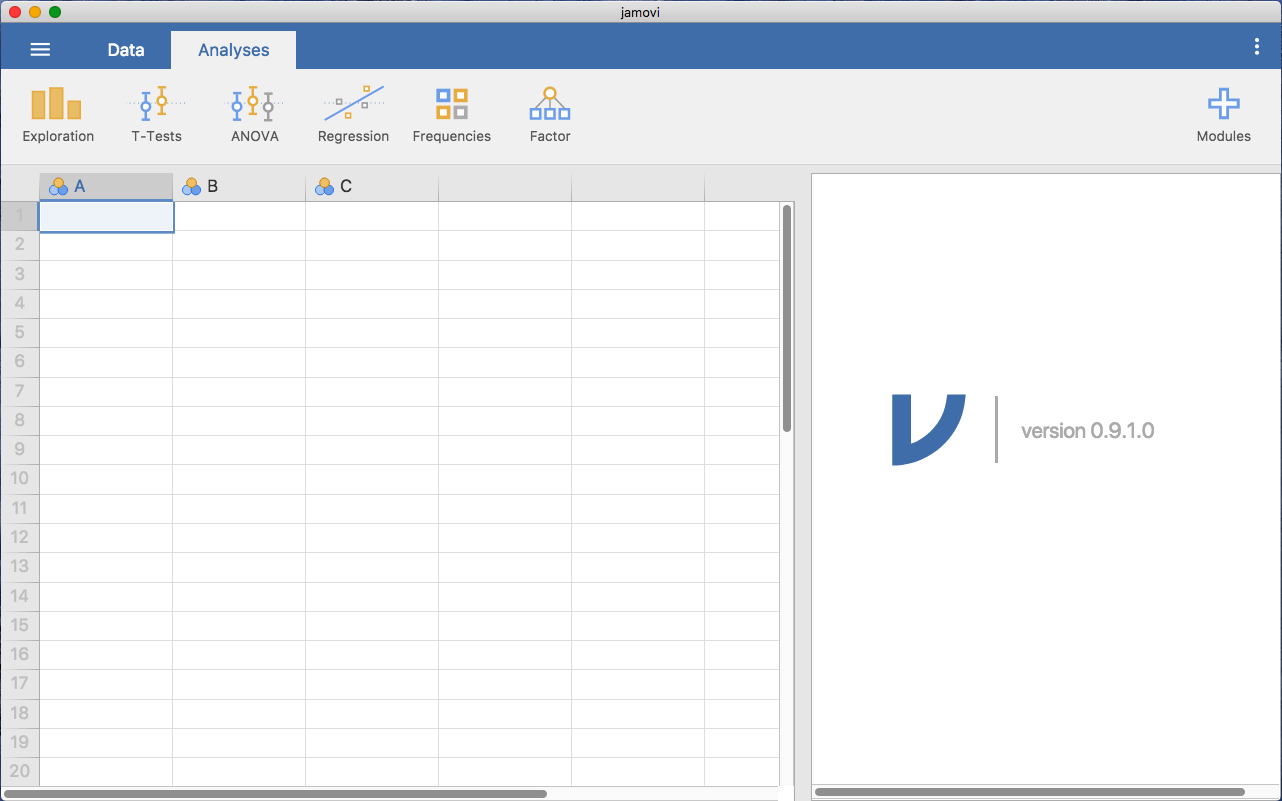
\includegraphics[width=17.81in]{img/introj/startingjamovi} \caption{ jamovi looks like this when you start it}\label{fig:startingjamovi}
\end{figure}

To the left is the spreadsheet view, and to the right is where the results of statistical tests appear. Down the middle is a bar separating these two regions and this can be dragged to the left or the right to change their sizes.

It is possible to simply begin typing values into the jamovi spreadsheet as you would in any other spreadsheet software. Alternatively, existing data sets in the CSV (.csv) file format can be opened in jamovi. Additionally, you can easily import SPSS, SAS, Stata and JASP files directly into jamovi. To open a file select the File tab (three horizontal lines signify this tab) at the top left hand corner, select `Open' and then choose from the files listed on `Browse' depending on whether you want to open an example or a file stored on your computer.

\hypertarget{analyses}{%
\section{Analyses}\label{analyses}}

Analyses can be selected from the analysis ribbon or menu along the top. Selecting an analysis will present an `options panel' for that particular analysis, allowing you to assign different variables to different parts of the analysis, and select different options. At the same time, the results for the analysis will appear in the right `Results panel' and will update in real-time as you make changes to the options.

When you have the analysis set up correctly you can dismiss the analysis options by clicking the arrow to the top right of the optional panel. If you wish to return to these options, you can click on the results that were produced. In this way, you can return to any analysis that you (or say, a colleague) created earlier.

If you decide you no longer need a particular analysis, you can remove it with the results context menu. Right-clicking on the analysis results will bring up a menu and by selecting `Analysis' and then `Remove' the analysis can be removed. But more on this later. First, let's take a more detailed look at the spreadsheet view.

\hypertarget{spreadsheet}{%
\section{The spreadsheet}\label{spreadsheet}}

In jamovi data is represented in a spreadsheet with each column representing a `variable' and each row representing a `case' or `participant'.

\hypertarget{variables}{%
\subsection{Variables}\label{variables}}

The most commonly used variables in jamovi are `Data Variables', these variables simply contain data either loaded from a data file, or `typed in' by the user. Data variables can be one of three measurement levels:

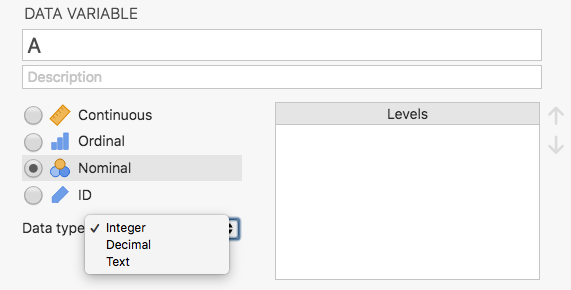
\includegraphics[width=7.93in]{img/introj/measurementlevels}

These levels are designated by the symbol in the header of the variable's column.

The \emph{ID} variable type is unique to jamovi. It's intended for variables that contain identifiers that you would almost never want to analyse. For example, a persons name, or a participant ID. Specifying an ID variable type can improve performance when interacting with very large data sets.

\begin{itemize}
\tightlist
\item
  \emph{Nominal} variables are for categorical variables which are text labels, for example a column called Gender with the values Male and Female would be nominal. So would a person's name. Nominal variable values can also have a numeric value. These variables are used most often when importing data which codes values with numbers rather than text. For example, a column in a dataset may contain the values 1 for males, and 2 for females. It is possible to add nice `human-readable' labels to these values with the variable editor (more on this later).
\item
  \emph{Ordinal} variables are like Nominal variables, except the values have a specific order. An example is a Likert scale with 3 being `strongly agree' and -3 being `strongly disagree'.
\item
  \emph{Continuous} variables are variables which exist on a continuous scale. Examples might be height or weight. This is also referred to as `Interval' or `Ratio scale'.
\end{itemize}

In addition, you can also specify different data types: variables have a data type of either `Text', `Integer' or `Decimal'.

When starting with a blank spreadsheet and typing values in the variable type will change automatically depending on the data you enter. This is a good way to get a feel for which variable types go with which sorts of data. Similarly, when opening a data file jamovi will try and guess the variable type from the data in each column. In both cases this automatic approach may not be correct, and it may be necessary to manually specify the variable type with the variable editor.

The variable editor can be opened by selecting `Setup' from the data tab or by double-clicking on the variable column header. The variable editor allows you to change the name of the variable and, for data variables, the variable type, the order of the levels, and the label displayed for each level. Changes can be applied by clicking the `tick' to the top right. The variable editor can be dismissed by clicking the `Hide' arrow.

New variables can be inserted or appended to the data set using the `add' button from the data ribbon. The `add' button also allows the addition of computed variables.

\hypertarget{computed-variables}{%
\subsection{Computed variables}\label{computed-variables}}

Computed Variables are those which take their value by performing a computation on other variables. Computed Variables can be used for a range of purposes, including log transforms, z-scores, sum-scores, negative scoring and means.

Computed variables can be added to the data set with the `add' button available on the data tab. This will produce a formula box where you can specify the formula. The usual arithmetic operators are available. Some examples of formulas are:

\texttt{A\ +\ B}

\texttt{LOG10(len)}

\texttt{MEAN(A,\ B)}

\texttt{(dose\ -\ VMEAN(dose))\ /\ VSTDEV(dose)}

In order, these are the sum of A and B, a log (base 10) transform of len, the mean of A and B, and the z-score of the variable dose. Figure \ref{fig:computedvariable} below shows the jamovi screen for the new variable computed as the z-score of dose (from the `Tooth Growth' example data set).

\begin{figure}
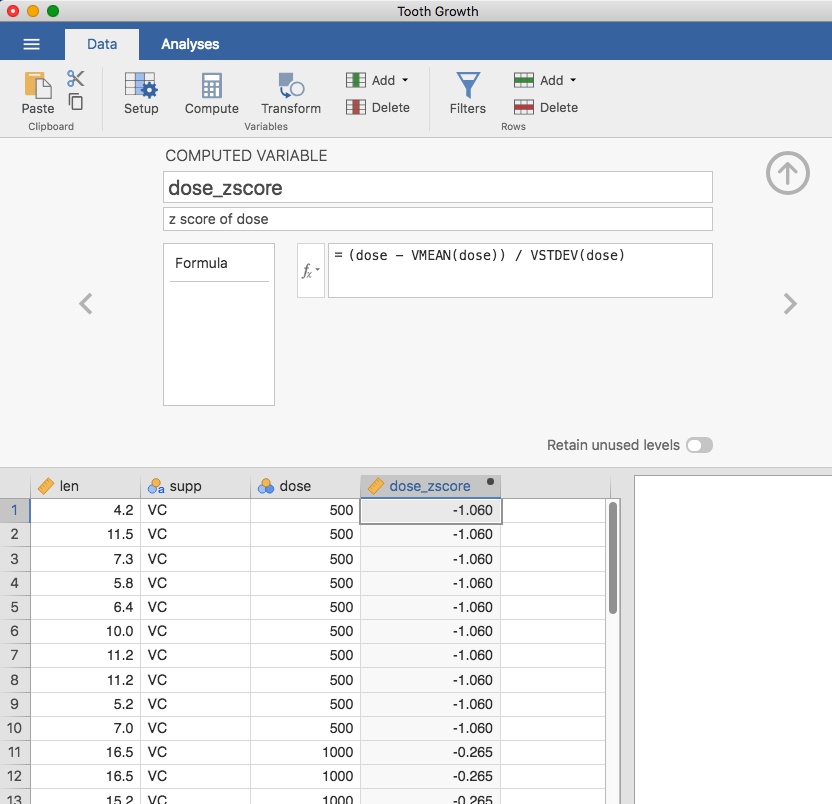
\includegraphics[width=11.56in]{img/introj/computedvariable} \caption{A newly computed variable, the z-score of ‘dose’}\label{fig:computedvariable}
\end{figure}

\emph{V-functions}
Several functions are already available in jamovi and available from the drop down box labelled \emph{f\textsubscript{x}}. A number of functions appear in pairs, one prefixed with a V and the other not. V functions perform their calculation on a variable as a whole, where as non-V functions perform their calculation row by row. For example, MEAN(A, B) will produce the mean of A and B for each row. Where as VMEAN(A) gives the mean of all the values in A.

\hypertarget{copypaste}{%
\subsection{Copy and Paste}\label{copypaste}}

jamovi produces nice American Psychological Association (APA) formatted tables and attractive plots. It is often useful to be able to copy and paste these, perhaps into a Word document, or into an email to a colleague. To copy results right click on the object of interest and from the menu select exactly what you want to copy. The menu allows you to choose to copy only the image or the entire analysis. Selecting ``copy'' copies the content to the clipboard and this can be pasted into other programs in the usual way. You can practice this later on when we do some analyses.

\hypertarget{syntaxmode}{%
\subsection{Syntax mode}\label{syntaxmode}}

jamovi also provides an ``R Syntax Mode''. In this mode jamovi produces equivalent R code for each analysis. To change to syntax mode, select the Application menu to the top right of jamovi (a button with three vertical dots) and click the ``Syntax mode'' checkbox there. You can turn off syntax mode by clicking this a second time.

In syntax mode analyses continue to operate as before but now they produce R syntax, and `ascii output' like an R session. Like all results objects in jamovi, you can right click on these items (including the R syntax) and copy and paste them, for example into an R session. At present, the provided R syntax does not include the data import step and so this must be performed manually in R. There are many resources explaining how to import data into R and if you are interested we recommend you take a look at these; just search on the interweb.

\hypertarget{load}{%
\section{Loading data in jamovi}\label{load}}

There are several different types of files that are likely to be relevant to us when doing data analysis. There are two in particular that are especially important from the perspective of this book:

\begin{itemize}
\tightlist
\item
  \emph{jamovi files} are those with a \texttt{.omv} file extension. This is the standard kind of file that jamovi uses to store data, and variables and analyses.
\item
  Comma separated value (csv) files\} are those with a \texttt{.csv} file extension. These are just regular old text files and they can be opened with many different software programs. It's quite typical for people to store data in csv files, precisely because they're so simple.
\end{itemize}

There are also several other kinds of data file that you might want to import into jamovi. For instance, you might want to open Microsoft Excel spreadsheets \texttt{.xls} files), or data files that have been saved in the native file formats for other statistics software, such as SPSS or SAS. Whichever file formats you are using, it's a good idea to create a folder or folders especially for your jamovi data sets and analyses and to make sure you keep these backed up regularly.

\hypertarget{importing-data-from-csv-files}{%
\subsection{Importing data from csv files}\label{importing-data-from-csv-files}}

One quite commonly used data format is the humble ``comma separated value'' file, also called a csv file, and usually bearing the file extension \texttt{.csv}. csv files are just plain old-fashioned text files and what they store is basically just a table of data. This is illustrated in Figure \ref{fig:booksalescsv}, which shows a file called \texttt{booksales.csv} that I've created. As you can see, each row represents the book sales data for one month. The first row doesn't contain actual data though, it has the names of the variables.

\begin{figure}
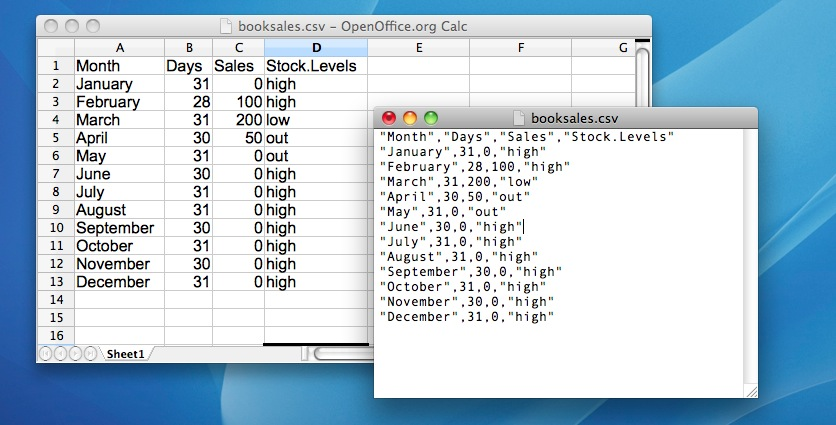
\includegraphics[width=11.61in]{img/mechanics/booksalescsv} \caption{The booksales.csv data file. On the left I’ve opened the file using a spreadsheet program (OpenOffice), which shows that the file is basically a table. On the right the same file is open in a standard text editor (the TextEdit program on a Mac), which shows how the file is formatted. The entries in the table are wrapped in quote marks and separated by commas.}\label{fig:booksalescsv}
\end{figure}

It's easy to open csv files in jamovi. From the top left menu (the button with three parallel lines) choose `Open' and browse to where you have stored the csv file on your computer. If you're on a Mac, it'll look like the usual Finder window that you use to choose a file; on Windows it looks like an Explorer window. An example of what it looks like on a Mac is shown in Figure \ref(fig:fileopen). I'm assuming that you're familiar with your own computer, so you should have no problem finding the csv file that you want to import! Find the one you want, then click on the `Open' button.

\begin{figure}
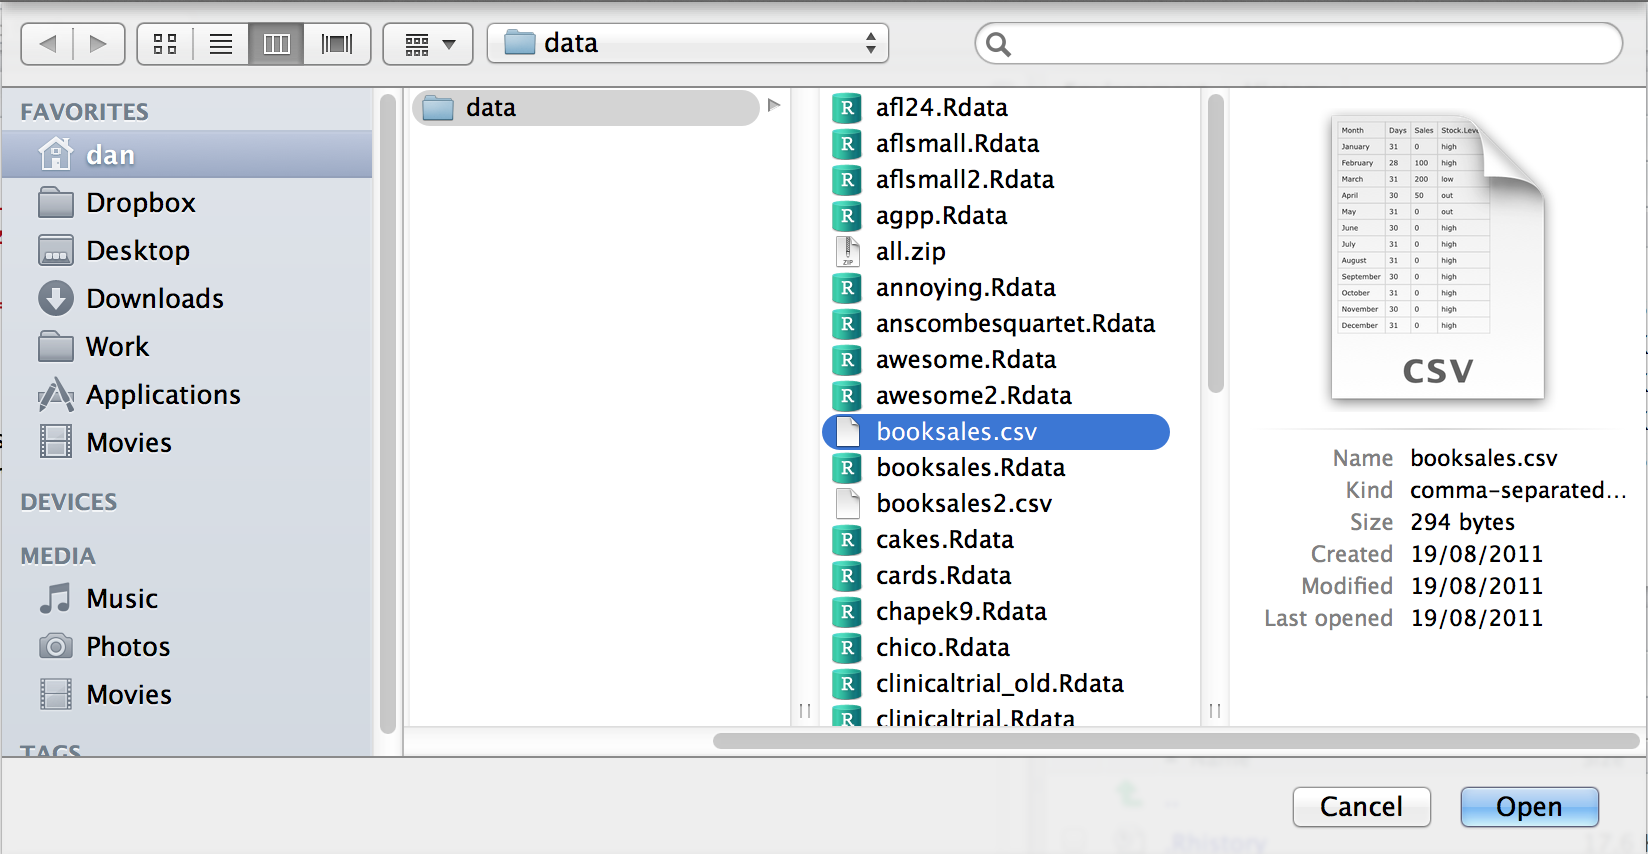
\includegraphics[width=22.89in]{img/mechanics/openscreen} \caption{A dialog box on a Mac asking you to select the csv file jamovi should try to import. Mac users will recognise this immediately, it’s the usual way in which a Mac asks you to find a file. Windows users won’t see this, instead they’ll see the usual explorer window that Windows always gives you when it wants you to select a file.}\label{fig:fileopen}
\end{figure}

There are a few things that you can check to make sure that the data gets imported correctly:

\begin{itemize}
\tightlist
\item
  Heading. Does the first row of the file contain the names for each variable - a ``header'' row? The \texttt{booksales.csv} file has a header, so that's a yes.
\item
  Separator. What character is used to separate different entries? In most csv files this will be a comma (it is ``comma separated'' after all).
\item
  Decimal. What character is used to specify the decimal point? In English speaking countries this is almost always a period (i.e., \texttt{.}). That's not universally true though, many European countries use a comma.
\item
  Quote. What character is used to denote a block of text? That's usually going to be a double quote mark ". It is for the \texttt{booksales.csv} file.
\end{itemize}

\hypertarget{importing}{%
\section{Importing unusual data files}\label{importing}}

Throughout this book I've assumed that your data are stored as a jamovi \texttt{.omv} file or as a ``properly''' formatted csv file. However, in real life that's not a terribly plausible assumption to make so I'd better talk about some of the other possibilities that you might run into.

\hypertarget{loading-data-from-text-files}{%
\subsection{Loading data from text files}\label{loading-data-from-text-files}}

The first thing I should point out is that if your data are saved as a text file but aren't \emph{quite} in the proper csv format then there's still a pretty good chance that jamovi will be able to open it. You just need to try it and see if it works. Sometimes though you will need to change some of the formatting. The ones that I've often found myself needing to change are:

\begin{itemize}
\tightlist
\item
  header. A lot of the time when you're storing data as a csv file the first row actually contains the column names and not data. If that's not true then it's a good idea to open up the csv file in a spreadsheet programme such as Open Office and add the header row manually.
\item
  sep. As the name ``comma separated value'' indicates, the values in a row of a csv file are usually separated by commas. This isn't universal, however. In Europe the decimal point is typically written as \texttt{,} instead of \texttt{.} and as a consequence it would be somewhat awkward to use \texttt{,} as the separator. Therefore it is not unusual to use \texttt{;} instead of \texttt{,} as the separator. At other times, I've seen a TAB character used.
\item
  quote. It's conventional in csv files to include a quoting character for textual data. As you can see by looking at the \texttt{booksales.csv} file, this is usually a double quote character, \texttt{"}. But sometimes there is no quoting character at all, or you might see a single quote mark \texttt{\textquotesingle{}} used instead.
\item
  skip. It's actually very common to receive CSV files in which the first few rows have nothing to do with the actual data. Instead, they provide a human readable summary of where the data came from, or maybe they include some technical info that doesn't relate to the data.
\item
  missing values. Often you'll get given data with missing values. For one reason or another, some entries in the table are missing. The data file needs to include a ``special'' value to indicate that the entry is missing. By default jamovi assumes that this value is \texttt{99}\footnote{You can change the default value for missing values in jamovi from the top right menu (three vertical dots), but this only works at the time of importing data files into jamovi. The default missing value in the dataset should not be a valid number associated with any of the variables, e.g.~you could use \texttt{-9999} as this is unlikely to be a valid value.}, for both numeric and text data, so you should make sure that, where necessary, all missing values in the csv file are replaced with \texttt{99} (or \texttt{-9999}; whichever you choose) before opening / importing the file into jamovi. Once you have opened / imported the file into jamovi all the missing values are converted to blank cells in the jamovi spreadsheet view.
\end{itemize}

\hypertarget{loading-data-from-spss-and-other-statistics-packages}{%
\subsection{Loading data from SPSS (and other statistics packages)}\label{loading-data-from-spss-and-other-statistics-packages}}

The commands listed above are the main ones we'll need for data files in this book. But in real life we have many more possibilities. For example, you might want to read data files in from other statistics programs. Since SPSS is probably the most widely used statistics package in psychology, it's worth mentioning that jamovi can also import SPSS data files (file extension \texttt{.sav}). Just follow the instructions above for how to open a csv file, but this time navigate to the .sav file you want to import. For SPSS files, jamovi will regard all values as missing if they are regarded as ``system missing'' files in SPSS. The `Default missings' value does not seem to work as expected when importing SPSS files, so be aware of this - you might need another step: import the SPSS file into jamovi, then export as a csv file before re-opening in jamovi.\footnote{I know this is a bot of a fudge, but it does work and hopefully this will be fixed in a later version of jamovi.}.

And that's pretty much it, at least as far as SPSS goes. As far as other statistical software goes, jamovi can also directly open / import SAS and STATA files.

\hypertarget{loading-excel-files}{%
\subsection{Loading Excel files}\label{loading-excel-files}}

A different problem is posed by Excel files. Despite years of yelling at people for sending data to me encoded in a proprietary data format, I get sent a lot of Excel files. The way to handle Excel files is to open them up first in Excel or another spreadsheet programme that can handle Excel files, and then export the data as a csv file before opening / importing the csv file into jamovi.

\hypertarget{coercion}{%
\section{Changing data from one level to another}\label{coercion}}

Sometimes you want to change the variable level. This can happen for all sorts of reasons. Sometimes when you import data from files, it can come to you in the wrong format. Numbers sometimes get imported as nominal, text values. Dates may get imported as text. ParticipantID values can sometimes be read as continuous: nominal values can sometimes be read as ordinal or even continuous. There's a good chance that sometimes you'll want to convert a variable from one measurement level into another one. Or, to use the correct term, you want to \textbf{\emph{coerce}} the variable from one class into another.

In \ref{spreadsheet} we saw how to specify different variable levels, and if you want to change a variable's measurement level then you can do this in the jamovi data view for that variable. Just click the check box for the measurement level you want - continuous, ordinal, or nominal.

\hypertarget{jamovimodules}{%
\section{Installing add-on modules into jamovi}\label{jamovimodules}}

A really great feature of jamovi is the ability to install add-on modules from the jamovi library. These add-on modules have been developed by the jamovi community, i.e., jamovi users and developers who have created special software add-ons that do other, usually more advanced, analyses that go beyond the capabilities of the base jamovi program.

To install add-on modules, just click on the large ``+'' in the top right of the jamovi window, select `jamovi-library' and then browse through the various add-on modules that are available. Choose the one(s) you want, and then install them, as in Figure \ref{fig:modules}. It's that easy. The newly installed modules can then be accessed from the ``Analyses'' button bar. Try it\ldots useful add-on modules to install include ``scatr'' (added under ``Descriptives'') and ``R j''.

\begin{figure}
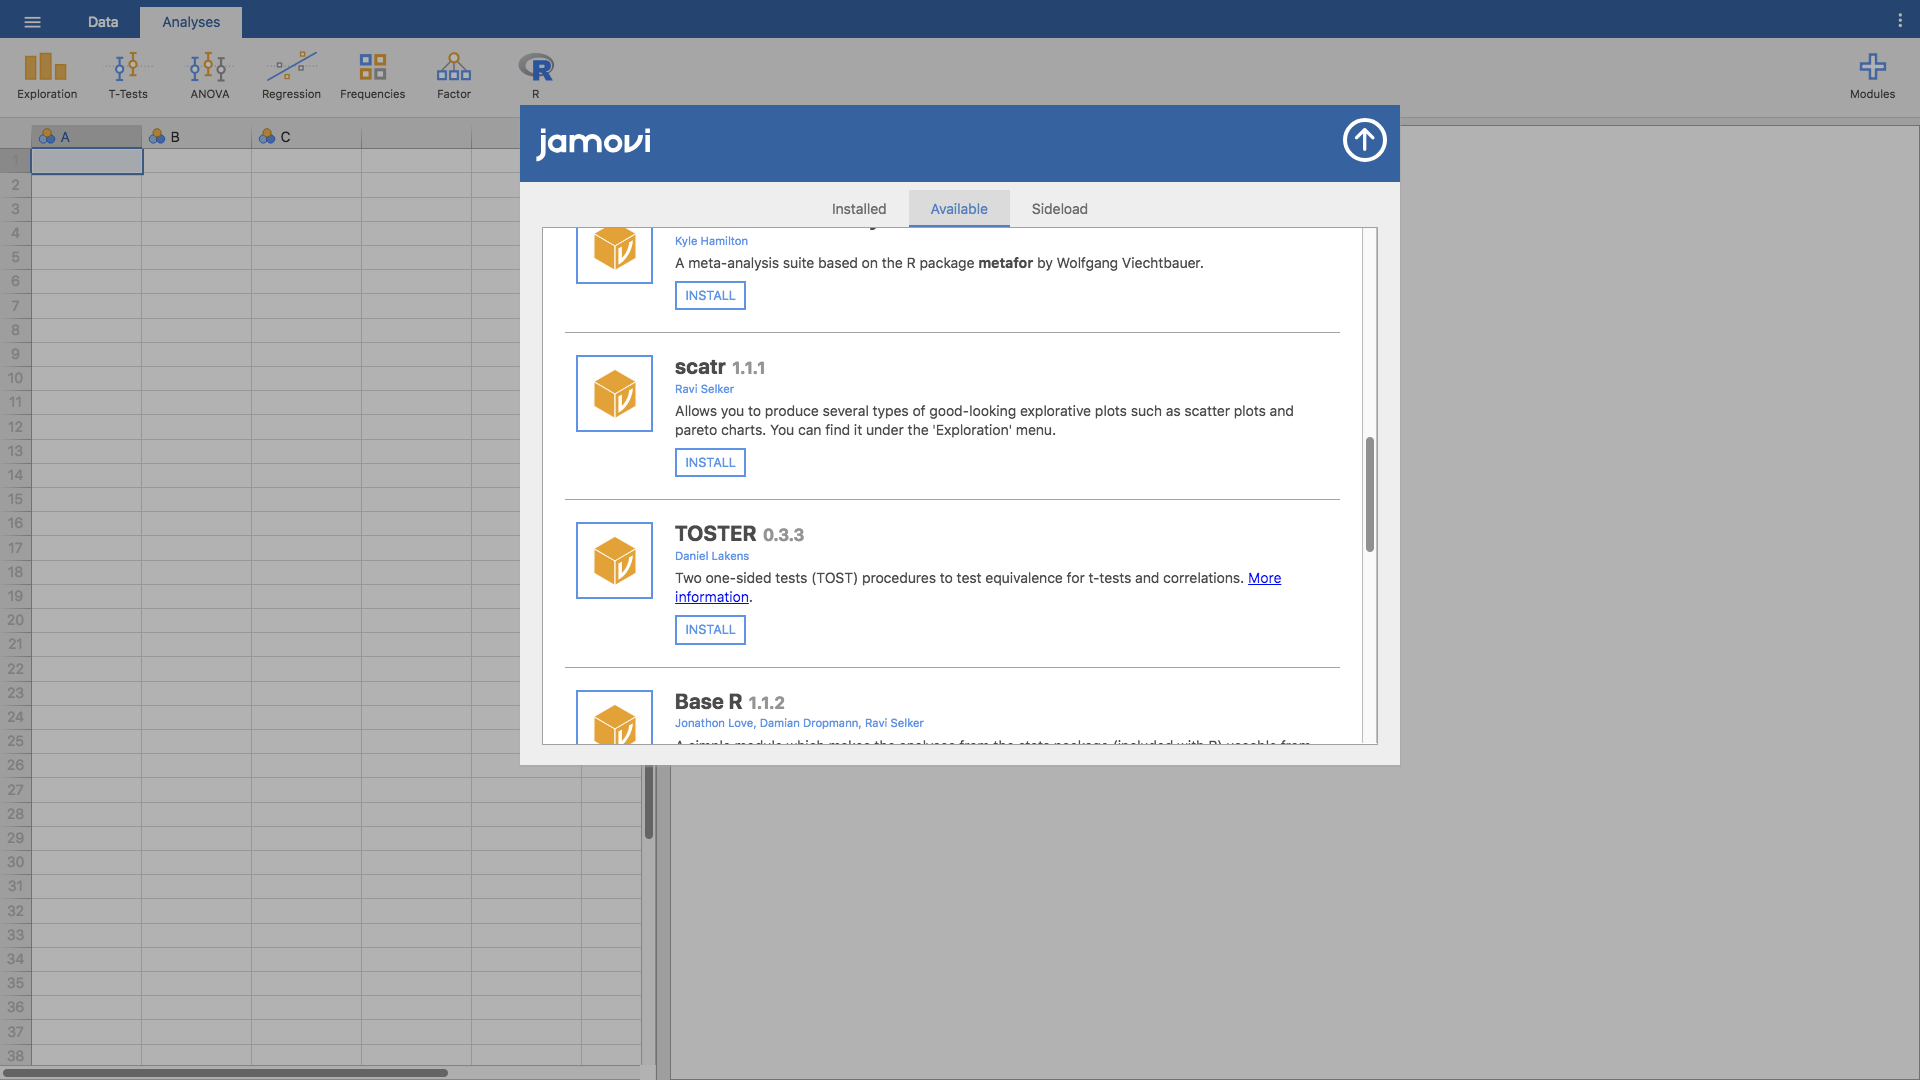
\includegraphics[width=26.67in]{img/graphics/modules} \caption{Installing add-on modules in jamovi}\label{fig:modules}
\end{figure}

\hypertarget{quittingjamovi}{%
\section{Quitting jamovi}\label{quittingjamovi}}

There's one last thing I should cover in this chapter: how to quit jamovi. It's not hard, just close the program the same way you would any other program. However, what you might want to do before you quit is save your work! There are two parts to this: saving any changes to the data set, and saving the analyses that you ran.

It is good practice to save any changes to the data set as a \emph{new} data set. That way you can always go back to the original data. To save any changes in jamovi, select ``Export''\ldots{}``Data'' from the main jamovi menu (button with three horizontal bars in the top left) and create a new file name for the changed data set.

Alternatively, you can save \emph{both} the changed data and any analyses you have undertaken by saving as a jamovi file. To do this, from the main jamovi menu select ``Save as'' and type in a file name for this ``jamovi file (.omv)''. Remember to save the file in a location where you can find it again later. I usually create a new folder for specific data sets and analyses.

\hypertarget{summary-1}{%
\section{Summary}\label{summary-1}}

\begin{itemize}
\tightlist
\item
  Section \ref{gettingjamovi}. We downloaded and installed jamovi, and started it up.
\item
  Section \ref{analyses}. We very briefly oriented to the part of jamovi where analyses are done and results appear, but then deferred this until later in the book.
\item
  Section \ref{spreadsheet}. We spent more time looking at the spreadsheet part of jamovi, and considered different variable types, and how to compute new variables.
\item
  Section \ref{load}. We also saw how to load data files in jamovi.
\item
  Section \ref{importing}. Then we figured out how to open other data files, from different file types.
\item
  Section \ref{coercion}. And saw that sometimes we need to coerce data from one type to another.
\item
  Section \ref{jamovimodules}. Installing add-on modules from the jamovi community really extends jamovi capabilities.
\item
  Section \ref{quittingjamovi}. Finally, we looked at good practice in terms of saving your data set and analyses when you have finished and are about to quit jamovi.
\end{itemize}

\hypertarget{part-iii.-working-with-data}{%
\chapter*{Part III. Working with data}\label{part-iii.-working-with-data}}
\addcontentsline{toc}{chapter}{Part III. Working with data}

\hypertarget{descriptives}{%
\chapter{Descriptive statistics}\label{descriptives}}

Any time that you get a new data set to look at one of the first tasks that you have to do is find ways of summarising the data in a compact, easily understood fashion. This is what \textbf{\emph{descriptive statistics}} (as opposed to inferential statistics) is all about. In fact, to many people the term `statistics' is synonymous with descriptive statistics. It is this topic that we'll consider in this chapter, but before going into any details, let's take a moment to get a sense of why we need descriptive statistics. To do this, let's open the \texttt{aflsmall\_margins} file and see what variables are stored in the file.

\textbackslash begin\{figure\}
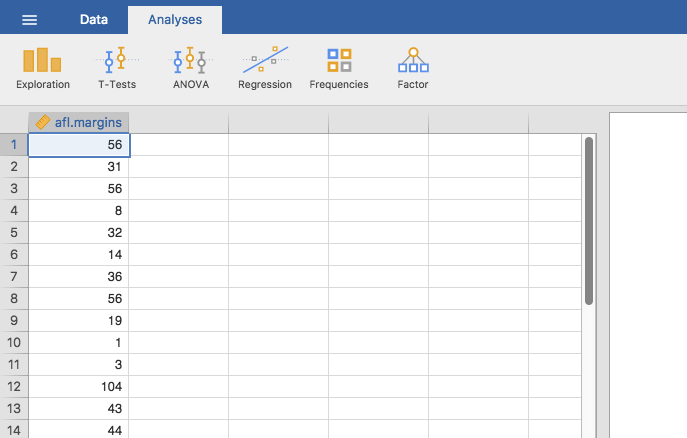
\includegraphics[width=9.54in]{img/descriptives/aflsmall_margins} \textbackslash caption\{A screenshot of jamovi showing the variables stored in the aflsmall\_margins.csv file\}\label{fig:aflsmall}
\textbackslash end\{figure\}

In fact, there is just one variable here, \texttt{afl.margins}. We'll focus a bit on this variable in this chapter, so I'd better tell you what it is. Unlike most of the data sets in this book, this is actually real data, relating to the Australian Football League (AFL).\footnote{Note for non-Australians: the AFL is an Australian rules football competition. You don't need to know anything about Australian rules in order to follow this section.} The \texttt{afl.margins} variable contains the winning margin (number of points) for all 176 home and away games played during the 2010 season.

This output doesn't make it easy to get a sense of what the data are actually saying. Just `looking at the data' isn't a terribly effective way of understanding data. In order to get some idea about what the data are actually saying we need to calculate some descriptive statistics (this chapter) and draw some nice pictures (Chapter \ref{graphics}). Since the descriptive statistics are the easier of the two topics I'll start with those, but nevertheless I'll show you a histogram of the \texttt{afl.margins} data since it should help you get a sense of what the data we're trying to describe actually look like, see Figure \ref{fig:histogram1}. We'll talk a lot more about how to draw histograms in Section \ref{sec:hist}. For now, it's enough to look at the histogram and note that it provides a fairly interpretable representation of the \texttt{afl.margins} data.

\begin{figure}
\centering
\includegraphics{img/descriptives/aflMargins.eps}
\caption{\label{fig:histogram1}A histogram of the AFL 2010 winning margin data (the afl.margins variable). As you might expect, the larger the winning margin the less frequently you tend to see it.}
\end{figure}

\hypertarget{centraltendency}{%
\section{Measures of central tendency}\label{centraltendency}}

Drawing pictures of the data, as I did in Figure \ref{fig:histogram1}, is an excellent way to convey the `gist' of what the data is trying to tell you. It's often extremely useful to try to condense the data into a few simple `summary' statistics. In most situations, the first thing that you'll want to calculate is a measure of \textbf{\emph{central tendency}}. That is, you'd like to know something about where the `average' or `middle' of your data lies. The three most commonly used measures are the mean, median and mode. I'll explain each of these in turn, and then discuss when each of them is useful.

\hypertarget{mean}{%
\subsection{The mean}\label{mean}}

The \textbf{\emph{mean}} of a set of observations is just a normal, old-fashioned average. Add all of the values up, and then divide by the total number of values. The first five AFL winning margins were 56, 31, 56, 8 and 32, so the mean of these observations is just:
\[
\frac{56 + 31 + 56 + 8 + 32}{5} = \frac{183}{5} = 36.60
\]
Of course, this definition of the mean isn't news to anyone. Averages (i.e., means) are used so often in everyday life that this is pretty familiar stuff. However, since the concept of a mean is something that everyone already understands, I'll use this as an excuse to start introducing some of the mathematical notation that statisticians use to describe this calculation, and talk about how the calculations would be done in jamovi.

The first piece of notation to introduce is \(N\), which we'll use to refer to the number of observations that we're averaging (in this case \(N = 5\)). Next, we need to attach a label to the observations themselves. It's traditional to use \(X\) for this, and to use subscripts to indicate which observation we're actually talking about. That is, we'll use \(X_1\) to refer to the first observation, \(X_2\) to refer to the second observation, and so on all the way up to \(X_N\) for the last one. Or, to say the same thing in a slightly more abstract way, we use \(X_i\) to refer to the \(i\)-th observation. Just to make sure we're clear on the notation, the following table lists the 5 observations in the \texttt{afl.margins} variable, along with the mathematical symbol used to refer to it and the actual value that the observation corresponds to:

\begin{center}
\begin{tabular}{ccc}
the observation & its symbol & the observed value \\ \hline
winning margin, game 1 & $X_1$ & 56 points \\
winning margin, game 2 & $X_2$ & 31 points \\
winning margin, game 3 & $X_3$ & 56 points \\
winning margin, game 4 & $X_4$ & 8 points \\
winning margin, game 5 & $X_5$ & 32 points \\
\end{tabular}
\end{center}

Okay, now let's try to write a formula for the mean. By tradition, we use \(\bar{X}\) as the notation for the mean. So the calculation for the mean could be expressed using the following formula:
\[
\bar{X} = \frac{X_1 + X_2 + \ldots + X_{N-1} + X_N}{N}
\]
This formula is entirely correct but it's terribly long, so we make use of the \keyterm{summation symbol} \(\scriptstyle\sum\) to shorten it.\footnote{The choice to use \(\Sigma\) to denote summation isn't arbitrary. It's the Greek upper case letter sigma, which is the analogue of the letter S in that alphabet. Similarly, there's an equivalent symbol used to denote the multiplication of lots of numbers, because multiplications are also called `products' we use the \(\Pi\) symbol for this (the Greek upper case pi, which is the analogue of the letter P).} If I want to add up the first five observations I could write out the sum the long way, \(X_1 + X_2 + X_3 + X_4 +X_5\) or I could use the summation symbol to shorten it to this:
\[
\sum_{i=1}^5 X_i
\]
Taken literally, this could be read as `the sum, taken over all \(i\) values from 1 to 5, of the value \(X_i\)'. But basically what it means is `add up the first five observations'. In any case, we can use this notation to write out the formula for the mean, which looks like this:
\[
\bar{X} = \frac{1}{N} \sum_{i=1}^N X_i 
\]

In all honesty, I can't imagine that all this mathematical notation helps clarify the concept of the mean at all. In fact, it's really just a fancy way of writing out the same thing I said in words: add all the values up and then divide by the total number of items. However, that's not really the reason I went into all that detail. My goal was to try to make sure that everyone reading this book is clear on the notation that we'll be using throughout the book: \(\bar{X}\) for the mean, \(\scriptstyle\sum\) for the idea of summation, \(X_i\) for the \(i\)th observation, and \(N\) for the total number of observations. We're going to be re-using these symbols a fair bit so it's important that you understand them well enough to be able to `read' the equations, and to be able to see that it's just saying `add up lots of things and then divide by another thing'.

\hypertarget{calculating-the-mean-in-jamovi}{%
\subsection{Calculating the mean in jamovi}\label{calculating-the-mean-in-jamovi}}

Okay, that's the maths. So how do we get the magic computing box to do the work for us? When the number of observations starts to become large it's much easier to do these sorts of calculations using a computer. To calculate the mean using all the data we can use jamovi. The first step is to click on the `Exploration' button and then click `Descriptives'. Then you can highlight the \texttt{afl.margins} variable and click the `right arrow' to move it across into the `Variables box'. As soon as you do that a Table appears on the right hand side of the screen containing default `Descriptives' information; see Figure @ref(fig:descriptives\_default).

\textbackslash begin\{figure\}
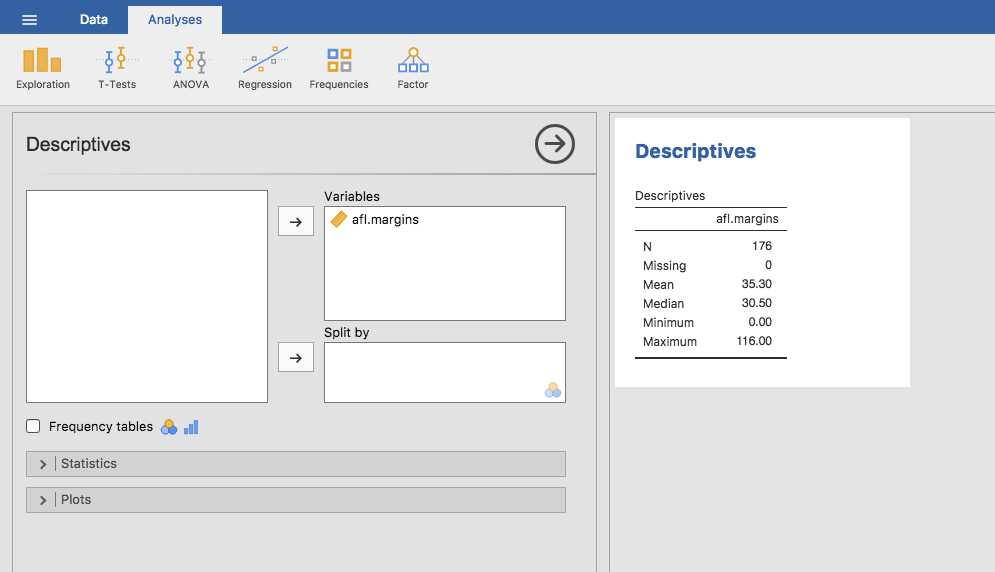
\includegraphics[width=13.82in]{img/descriptives/descriptives_default}

\caption{Default descriptives for the AFL 2010 winning margin data (the `afl.margins` variable).}

(\#fig:descriptives\_default)
\textbackslash end\{figure\}

As you can see in Figure @ref(fig:descriptives\_default), the mean value for the \texttt{afl.margins} variable is 35.30. Other information presented includes the total number of observations (N=176), the number of missing values (none), and the Median, Minimum and Maximum values for the variable.

\hypertarget{median}{%
\subsection{The median}\label{median}}

The second measure of central tendency that people use a lot is the \textbf{\emph{median}}, and it's even easier to describe than the mean. The median of a set of observations is just the middle value. As before let's imagine we were interested only in the first 5 AFL winning margins: 56, 31, 56, 8 and 32. To figure out the median we sort these numbers into ascending order:
\[
8, 31, \mathbf{32}, 56, 56
\]
From inspection, it's obvious that the median value of these 5 observations is 32 since that's the middle one in the sorted list (I've put it in bold to make it even more obvious). Easy stuff. But what should we do if we are interested in the first 6 games rather than the first 5? Since the sixth game in the season had a winning margin of 14 points, our sorted list is now
\[
8, 14, \mathbf{31}, \mathbf{32}, 56, 56
\]
and there are \emph{two} middle numbers, 31 and 32. The median is defined as the average of those two numbers, which is of course 31.5. As before, it's very tedious to do this by hand when you've got lots of numbers. In real life, of course, no-one actually calculates the median by sorting the data and then looking for the middle value. In real life we use a computer to do the heavy lifting for us, and jamovi has provided us with a Median value of 30.50 for the \texttt{afl.margins} variable (Figure @ref(fig:descriptives\_default)).

\hypertarget{mean-or-median-whats-the-difference}{%
\subsection{Mean or median? What's the difference?}\label{mean-or-median-whats-the-difference}}

Knowing how to calculate means and medians is only a part of the story. You also need to understand what each one is saying about the data, and what that implies for when you should use each one. This is illustrated in Figure \ref{fig:meanmedian}. The mean is kind of like the `centre of gravity' of the data set, whereas the median is the `middle value' in the data. What this implies, as far as which one you should use, depends a little on what type of data you've got and what you're trying to achieve. As a rough guide:

\begin{itemize}
\tightlist
\item
  If your data are nominal scale you probably shouldn't be using either the mean or the median. Both the mean and the median rely on the idea that the numbers assigned to values are meaningful. If the numbering scheme is arbitrary then it's probably best to use the mode (Section \ref{mode}) instead.
\item
  If your data are ordinal scale you're more likely to want to use the median than the mean. The median only makes use of the order information in your data (i.e., which numbers are bigger) but doesn't depend on the precise numbers involved. That's exactly the situation that applies when your data are ordinal scale. The mean, on the other hand, makes use of the precise numeric values assigned to the observations, so it's not really appropriate for ordinal data.
\item
  For interval and ratio scale data either one is generally acceptable. Which one you pick depends a bit on what you're trying to achieve. The mean has the advantage that it uses all the information in the data (which is useful when you don't have a lot of data). But it's very sensitive to extreme, outlying values.
\end{itemize}

\begin{figure}
\centering
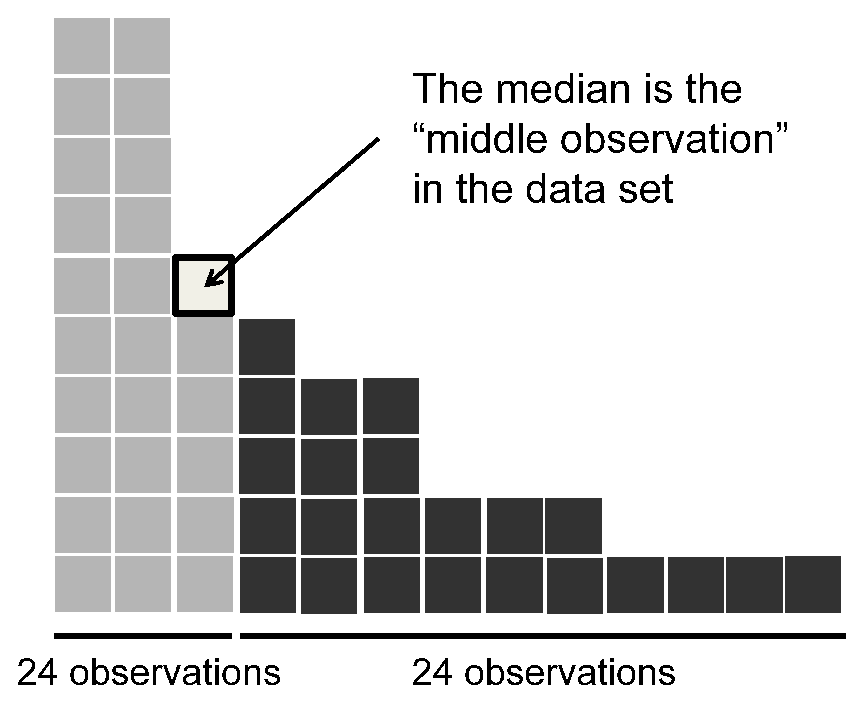
\includegraphics{img/descriptives2/median.eps}
\caption{\label{fig:meanmedian}An illustration of the difference between how the mean and the median should be interpreted. The mean is basically the `centre of gravity' of the data set. If you imagine that the histogram of the data is a solid object, then the point on which you could balance it (as if on a see-saw) is the mean. In contrast, the median is the middle observation, with half of the observations smaller and half of the observations larger.}
\end{figure}

Let's expand on that last part a little. One consequence is that there are systematic differences between the mean and the median when the histogram is asymmetric (skewed; see Section \ref{skewkurt}). This is illustrated in Figure \ref{fig:meanmedian}. Notice that the median (right hand side) is located closer to the `body' of the histogram, whereas the mean (left hand side) gets dragged towards the `tail' (where the extreme values are). To give a concrete example, suppose Bob (income \$50,000), Kate (income \$60,000) and Jane (income \$65,000) are sitting at a table. The average income at the table is \$58,333 and the median income is \$60,000. Then Bill sits down with them (income \$100,000,000). The average income has now jumped to \$25,043,750 but the median rises only to \$62,500. If you're interested in looking at the overall income at the table the mean might be the right answer. But if you're interested in what counts as a typical income at the table the median would be a better choice here.

\hypertarget{housingpriceexample}{%
\subsection{A real life example}\label{housingpriceexample}}

To try to get a sense of why you need to pay attention to the differences between the mean and the median let's consider a real life example. Since I tend to mock journalists for their poor scientific and statistical knowledge, I should give credit where credit is due. This is an excellent article on the ABC news website\footnote{\url{http://www.abc.net.au/news/stories/2010/09/24/3021480.htm}} from 24 September, 2010:

\begin{quote}
Senior Commonwealth Bank executives have travelled the world in the past couple of weeks with a presentation showing how Australian house prices, and the key price to income ratios, compare favourably with similar countries. ``Housing affordability has actually been going sideways for the last five to six years,'\,' said Craig James, the chief economist of the bank's trading arm, CommSec.
\end{quote}

This probably comes as a huge surprise to anyone with a mortgage, or who wants a mortgage, or pays rent, or isn't completely oblivious to what's been going on in the Australian housing market over the last several years. Back to the article:

\begin{quote}
CBA has waged its war against what it believes are housing doomsayers with graphs, numbers and international comparisons. In its presentation, the bank rejects arguments that Australia's housing is relatively expensive compared to incomes. It says Australia's house price to household income ratio of 5.6 in the major cities, and 4.3 nationwide, is comparable to many other developed nations. It says San Francisco and New York have ratios of 7, Auckland's is 6.7, and Vancouver comes in at 9.3.
\end{quote}

More excellent news! Except, the article goes on to make the observation that:

\begin{quote}
Many analysts say that has led the bank to use misleading figures and comparisons. If you go to page four of CBA's presentation and read the source information at the bottom of the graph and table, you would notice there is an additional source on the international comparison -- Demographia. However, if the Commonwealth Bank had also used Demographia's analysis of Australia's house price to income ratio, it would have come up with a figure closer to 9 rather than 5.6 or 4.3
\end{quote}

That's, um, a rather serious discrepancy. One group of people say 9, another says 4-5. Should we just split the difference and say the truth lies somewhere in between? Absolutely not! This is a situation where there is a right answer and a wrong answer. Demographia is correct, and the Commonwealth Bank is wrong. As the article points out:

\begin{quote}
{[}An{]} obvious problem with the Commonwealth Bank's domestic price to income figures is they compare average incomes with median house prices (unlike the Demographia figures that compare median incomes to median prices). The median is the mid-point, effectively cutting out the highs and lows, and that means the average is generally higher when it comes to incomes and asset prices, because it includes the earnings of Australia's wealthiest people. To put it another way: the Commonwealth Bank's figures count Ralph Norris' multi-million dollar pay packet on the income side, but not his (no doubt) very expensive house in the property price figures, thus understating the house price to income ratio for middle-income Australians.
\end{quote}

Couldn't have put it better myself. The way that Demographia calculated the ratio is the right thing to do. The way that the Bank did it is incorrect. As for why an extremely quantitatively sophisticated organisation such as a major bank made such an elementary mistake, well\ldots{} I can't say for sure since I have no special insight into their thinking. But the article itself does happen to mention the following facts, which may or may not be relevant:

\begin{quote}
{[}As{]} Australia's largest home lender, the Commonwealth Bank has one of the biggest vested interests in house prices rising. It effectively owns a massive swathe of Australian housing as security for its home loans as well as many small business loans.
\end{quote}

My, my.

\hypertarget{mode}{%
\subsection{Mode}\label{mode}}

The mode of a sample is very simple. It is the value that occurs most frequently. We can illustrate the mode using a different AFL variable: who has played in the most finals? Open the \texttt{aflsmall\_finalists} file and take a look at the \texttt{afl.finalists} variable, see Figure @ref(fig:aflsmall\_finalists). This variable contains the names of all 400 teams that played in all 200 finals matches played during the period 1987 to 2010.

\textbackslash begin\{figure\}
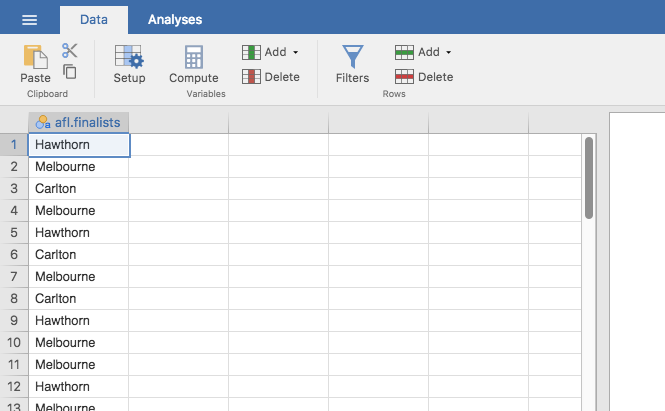
\includegraphics[width=9.24in]{img/descriptives/aflsmall_finalists} \textbackslash caption\{A screenshot of jamovi showing the variables stored in the aflsmall\_finalists.csv file\}(\#fig:aflsmall\_finalists)
\textbackslash end\{figure\}

What we \emph{could} do is read through all 400 entries and count the number of occasions on which each team name appears in our list of finalists, thereby producing a \textbf{\emph{frequency table}}. However, that would be mindless and boring: exactly the sort of task that computers are great at. So let's use jamovi to do this for us. Under `Exploration' - `Descriptives' click the small check box labelled `Frequency tables' and you should get something like Figure @ref(fig:aflsmall\_finalists\_mode).

\textbackslash begin\{figure\}
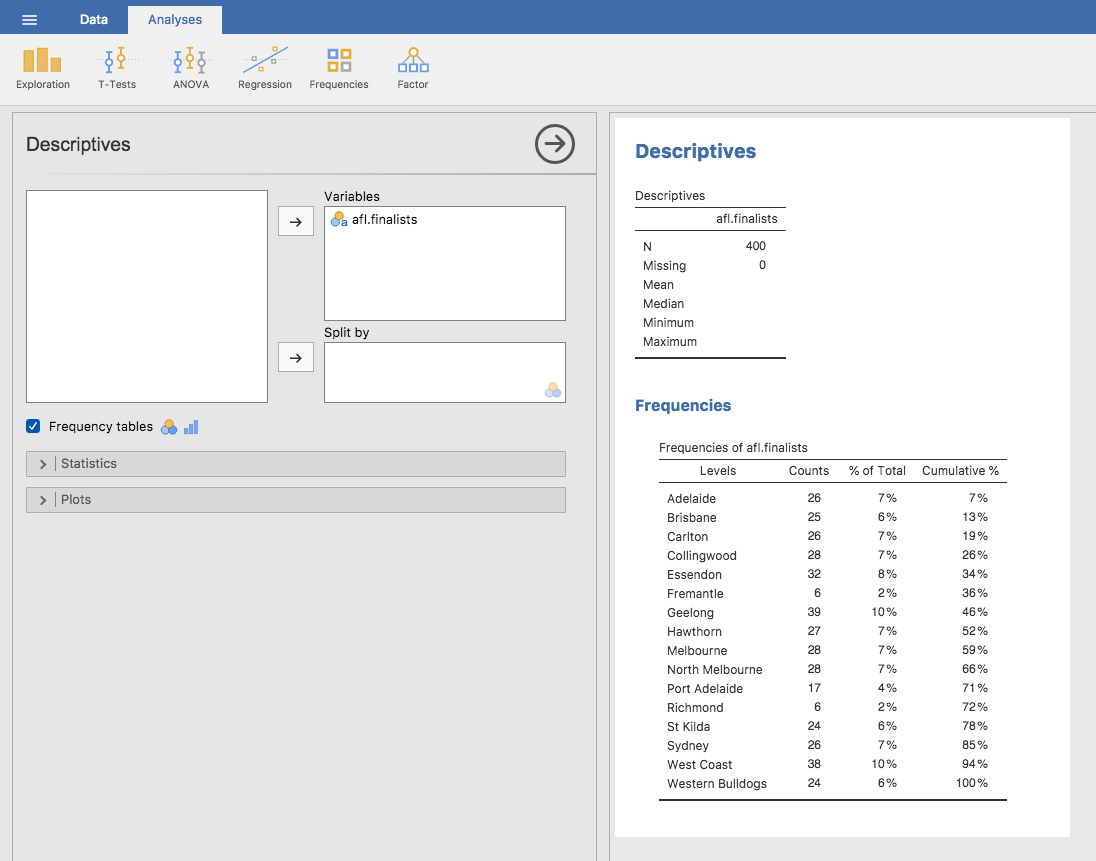
\includegraphics[width=15.22in]{img/descriptives/aflsmall_finalists_mode}

\caption{A screenshot of jamovi showing the frequency table for the afl.finalists variable}

(\#fig:aflsmall\_finalists\_mode)
\textbackslash end\{figure\}

Now that we have our frequency table we can just look at it and see that, over the 24 years for which we have data, Geelong has played in more finals than any other team. Thus, the mode of the \texttt{afl.finalists} data is \texttt{"Geelong"}. We can see that Geelong (39 finals) played in more finals than any other team during the 1987-2010 period. It's also worth noting that in the `Descriptives' Table no results are calculated for Mean, Median, Minimum or Maximum. This is because the \texttt{afl.finalists} variable is a nominal text variable so it makes no sense to calculate these values.

One last point to make regarding the mode. Whilst the mode is most often calculated when you have nominal data, because means and medians are useless for those sorts of variables, there are some situations in which you really do want to know the mode of an ordinal, interval or ratio scale variable. For instance, let's go back to our \texttt{afl.margins} variable. This variable is clearly ratio scale (if it's not clear to you, it may help to re-read Section \ref{scales}), and so in most situations the mean or the median is the measure of central tendency that you want. But consider this scenario: a friend of yours is offering a bet and they pick a football game at random. Without knowing who is playing you have to guess the \emph{exact} winning margin. If you guess correctly you win \$50. If you don't you lose \$1. There are no consolation prizes for \emph{almost} getting the right answer. You have to guess exactly the right margin. For this bet, the mean and the median are completely useless to you. It is the mode that you should bet on. To calculate the mode for the \texttt{afl.margins} variable in jamovi, go back to that data set and on the `Exploration' - `Descriptives' screen you will see you can expand the section marked `Statistics'. Click on the checkbox marked `Mode' and you will see the modal value presented in the `Descriptives' Table, as in Figure @ref(aflsmall\_margins\_mode). So the 2010 data suggest you should bet on a 3 point margin.

\textbackslash begin\{figure\}
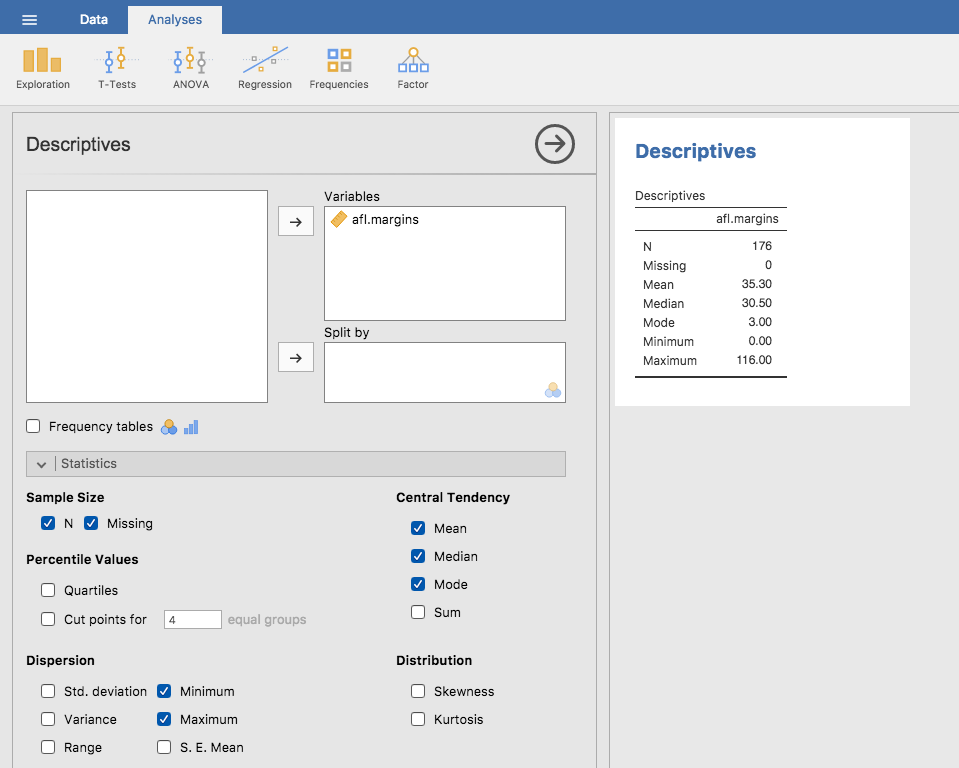
\includegraphics[width=13.32in]{img/descriptives/aflsmall_margins_mode}

\caption{A screenshot of jamovi showing the modal value for the afl.margins variable}

(\#fig:aflsmall\_margins\_mode)
\textbackslash end\{figure\}

\hypertarget{var}{%
\section{Measures of variability}\label{var}}

The statistics that we've discussed so far all relate to \{\it central tendency\}. That is, they all talk about which values are \texttt{in\ the\ middle\textquotesingle{}\textquotesingle{}\ or}popular'\,' in the data. However, central tendency is not the only type of summary statistic that we want to calculate. The second thing that we really want is a measure of the \keyterm{variability} of the data. That is, how \texttt{spread\ out\textquotesingle{}\textquotesingle{}\ are\ the\ data?\ How}far'\,' away from the mean or median do the observed values tend to be? For now, let's assume that the data are interval or ratio scale, and we'll continue to use the \rtext{afl.margins} data. We'll use this data to discuss several different measures of spread, each with different strengths and weaknesses.

\hypertarget{range}{%
\subsection{Range}\label{range}}

The \textbf{\emph{range}} of a variable is very simple. It's the biggest value minus the smallest value. For the AFL winning margins data the maximum value is 116 and the minimum value is 0. Although the range is the simplest way to quantify the notion of ``variability'\,', it's one of the worst. Recall from our discussion of the mean that we want our summary measure to be robust. If the data set has one or two extremely bad values in it we'd like our statistics to not be unduly influenced by these cases. For example, in a variable containing very extreme outliers
\[
-100,2,3,4,5,6,7,8,9,10
\]
it is clear that the range is not robust. This variable has a range of 110 but if the outlier were removed we would have a range of only 8.

\hypertarget{interquartile-range}{%
\subsection{Interquartile range}\label{interquartile-range}}

The \textbf{\emph{interquartile range}} (IQR) is like the range, but instead of the difference between the biggest and smallest value the difference between the 25th percentile and the 75th percentile is taken. If you don't already know what a \textbf{\emph{percentile}} is, the 10th percentile of a data set is the smallest number \(x\) such that 10\% of the data is less than \(x\). In fact, we've already come across the idea. The median of a data set is its 50th percentile! In jamovi you can easily specify the 25th, 50th and 75th percentiles by clicking the checkbox `Quartiles' in the `Exploration' - `Descriptives' - `Statistics' screen.

\textbackslash begin\{figure\}
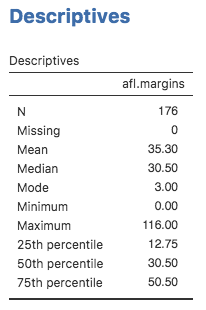
\includegraphics[width=2.86in]{img/descriptives/aflsmall_margins_iqr}

\caption{A screenshot of jamovi showing the Quartiles for the afl.margins variable }

(\#fig:aflsmall\_margins\_iqr)
\textbackslash end\{figure\}

And not surprisingly, in Figure @ref(fig:aflsmall\_margins\_iqr) the 50th percentile is the same as the median value. And, by noting that \(50.50 - 12.75 = 37.75\), we can see that the interquartile range for the 2010 AFL winning margins data is 37.75. While it's obvious how to interpret the range it's a little less obvious how to interpret the IQR. The simplest way to think about it is like this: the interquartile range is the range spanned by the `middle half' of the data. That is, one quarter of the data falls below the 25th percentile and one quarter of the data is above the 75th percentile, leaving the `middle half' of the data lying in between the two. And the IQR is the range covered by that middle half.

\hypertarget{aad}{%
\subsection{Mean absolute deviation}\label{aad}}

The two measures we've looked at so far, the range and the interquartile range, both rely on the idea that we can measure the spread of the data by looking at the percentiles of the data. However, this isn't the only way to think about the problem. A different approach is to select a meaningful reference point (usually the mean or the median) and then report the `typical' deviations from that reference point. What do we mean by `typical' deviation? Usually, this is the mean or median value of these deviations. In practice, this leads to two different measures: the `mean absolute deviation' (from the mean) and the `median absolute deviation' (from the median). From what I've read, the measure based on the median seems to be used in statistics and does seem to be the better of the two. But to be honest I don't think I've seen it used much in psychology. The measure based on the mean does occasionally show up in psychology though. In this section I'll talk about the first one, and I'll come back to talk about the second one later.

Since the previous paragraph might sound a little abstract, let's go through the \textbf{\emph{mean absolute deviation}} from the mean a little more slowly. One useful thing about this measure is that the name actually tells you exactly how to calculate it. Let's think about our AFL winning margins data, and once again we'll start by pretending that there are only 5 games in total, with winning margins of 56, 31, 56, 8 and 32. Since our calculations rely on an examination of the deviation from some reference point (in this case the mean), the first thing we need to calculate is the mean, \(\bar{X}\). For these five observations, our mean is \(\bar{X} = 36.6\). The next step is to convert each of our observations \(X_i\) into a deviation score. We do this by calculating the difference between the observation \(X_i\) and the mean \(\bar{X}\). That is, the deviation score is defined to be \(X_i - \bar{X}\). For the first observation in our sample, this is equal to \(56 - 36.6 = 19.4\). Okay, that's simple enough. The next step in the process is to convert these deviations to absolute deviations, and we do this by converting any negative values to positive ones. Mathematically, we would denote the absolute value of \(-3\) as \(|-3|\), and so we say that \(|-3| = 3\). We use the absolute value here because we don't really care whether the value is higher than the mean or lower than the mean, we're just interested in how \emph{close} it is to the mean. To help make this process as obvious as possible, the table below shows these calculations for all five observations:

\vspace{0.5cm}
\begin{center}
\begin{tabular}{ccccc} 
English: & which game & value & deviation from mean & absolute deviation \\
notation: & $i$ & $X_i$ & $X_i - \bar{X}$ &  $|X_i - \bar{X}|$ \\ \hline
& 1 & 56 & 19.4  & 19.4\\
& 2 & 31 &  -5.6 & 5.6\\ 
& 3 & 56 & 19.4  & 19.4\\
& 4 & 8 & -28.6  & 28.6\\
& 5 & 32 & -4.6  & 4.6 \\
\end{tabular}
\end{center}

Now that we have calculated the absolute deviation score for every observation in the data set, all that we have to do to calculate the mean of these scores. Let's do that:

\[
\frac{19.4 + 5.6 + 19.4 + 28.6 + 4.6}{5} = 15.52
\]

And we're done. The mean absolute deviation for these five scores is 15.52.

However, whilst our calculations for this little example are at an end, we do have a couple of things left to talk about. First, we should really try to write down a proper mathematical formula. But in order do to this I need some mathematical notation to refer to the mean absolute deviation. Irritatingly, `mean absolute deviation' and `median absolute deviation' have the same acronym (MAD), which leads to a certain amount of ambiguity so I'd better come up with something different for the mean absolute deviation. Sigh. What I'll do is use AAD instead, short for \emph{average} absolute deviation. Now that we have some unambiguous notation, here's the formula that describes what we just calculated:
\[
\mbox{\textsc{aad}}(X) = \frac{1}{N} \sum_{i = 1}^N |X_i - \bar{X}|
\]

\hypertarget{variance}{%
\subsection{Variance}\label{variance}}

Although the average absolute deviation measure has its uses, it's not the best measure of variability to use. From a purely mathematical perspective there are some solid reasons to prefer squared deviations rather than absolute deviations. If we do that we obtain a measure called the \textbf{\emph{variance}}, which has a lot of really nice statistical properties that I'm going to ignore,\footnote{Well, I will very briefly mention the one that I think is coolest, for a very particular definition of `cool', that is. Variances are \emph{additive}. Here's what that means. Suppose I have two variables \(X\) and \(Y\), whose variances are \(\mbox{Var}(X)\) and \(\mbox{Var}(Y)\) respectively. Now imagine I want to define a new variable \(Z\) that is the sum of the two, \(Z = X+Y\). As it turns out, the variance of \(Z\) is equal to \(\mbox{Var}(X) + \mbox{Var}(Y)\). This is a \emph{very} useful property, but it's not true of the other measures that I talk about in this section.} and one massive psychological flaw that I'm going to make a big deal out of in a moment. The variance of a data set \(X\) is sometimes written as \(\mbox{Var}(X)\), but it's more commonly denoted \(s^2\) (the reason for this will become clearer shortly).

The formula that we use to calculate the variance of a set of observations is as follows:
\[
\mbox{Var}(X) = \frac{1}{N} \sum_{i=1}^N \left( X_i - \bar{X} \right)^2
\]

As you can see, it's basically the same formula that we used to calculate the average absolute deviation, except that instead of using `absolute deviations' we use `squared deviations'. It is for this reason that the variance is sometimes referred to as the `mean square deviation'.

Now that we've got the basic idea, let's have a look at a concrete example. Once again, let's use the first five AFL games as our data. If we follow the same approach that we took last time, we end up with the following table:

\vspace{0.5cm}
\begin{center}
\begin{tabular}{ccccc} 
English: & which game & value & deviation from mean & squared deviation \\
maths: & $i$ & $X_i$ & $X_i - \bar{X}$ &  $(X_i - \bar{X})^2$ \\ \hline
& 1 & 56 & 19.4  & 376.36\\
& 2 & 31 &  -5.6 & 31.36\\ 
& 3 & 56 & 19.4  & 376.36\\
& 4 & 8 & -28.6  & 817.96\\
& 5 & 32 & -4.6  & 21.16 \\
\end{tabular}
\end{center}

That last column contains all of our squared deviations, so all we have to do is average them. If we do that by hand, i.e.~using a calculator, we end up with a variance of 324.64. Exciting, isn't it? For the moment, let's ignore the burning question that you're all probably thinking (i.e., what the heck does a variance of 324.64 actually mean?) and instead talk a bit more about how to do the calculations in jamovi, because this will reveal something very weird. Start a new jamovi session by clicking on the main menu button (three horizontal lines in the top left corner and selecting `New'. Now type in the first five values from the afl.margins data set in column A (\texttt{56,\ 31,\ 56,\ 8,\ 32}). Change the variable type to `Continuous' and under `Descriptives' click the `Variance' check box, and you get the same values for variance as the one we calculated by hand \texttt{324.64}). No, wait, you get a completely \emph{different} answer (\texttt{405.80}) - see Figure @ref(fig:aflsmall\_margins\_variance1). That's just weird. Is jamovi broken? Is this a typo? Am I an idiot?

\textbackslash begin\{figure\}
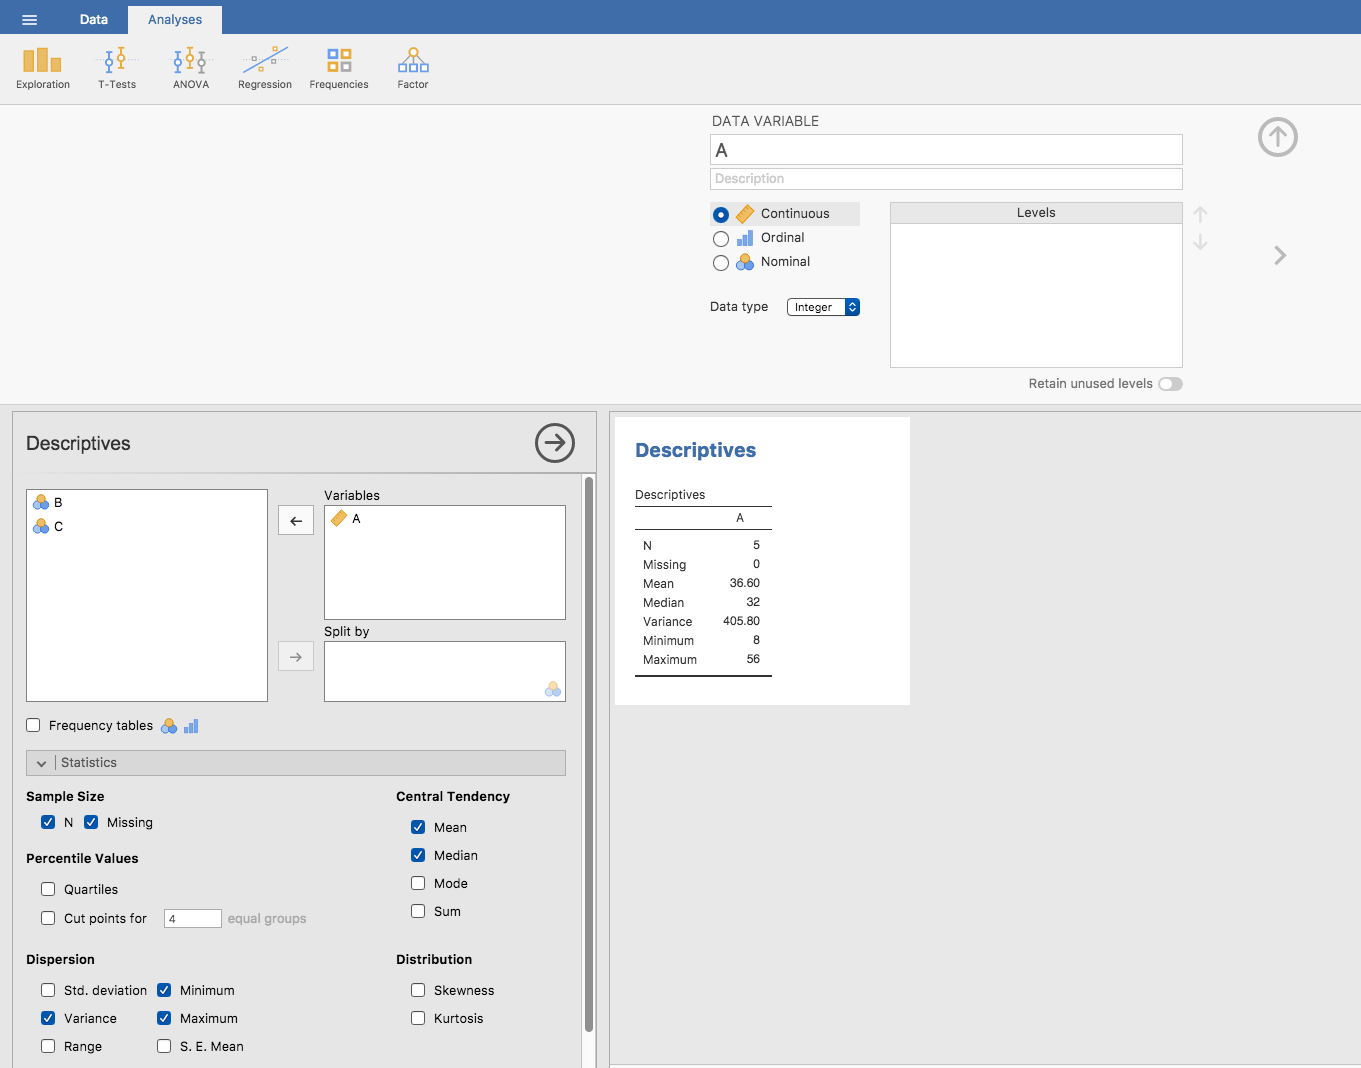
\includegraphics[width=18.9in]{img/descriptives/aflsmall_margins_variance1}

\caption{A screenshot of jamovi showing the Variance for the first 5 values of the afl.margins variable }

(\#fig:aflsmall\_margins\_variance1)
\textbackslash end\{figure\}

As it happens, the answer is no.\footnote{With the possible exception of the third question.}It's not a typo, and jamovi is not making a mistake. In fact, it's very simple to explain what jamovi is doing here, but slightly trickier to explain \emph{why} jamovi is doing it. So let's start with the `what'. What jamovi is doing is evaluating a slightly different formula to the one I showed you above. Instead of averaging the squared deviations, which requires you to divide by the number of data points \(N\), jamovi has chosen to divide by \(N-1\).

In other words, the formula that jamovi is using is this one:
\[
\frac{1}{N-1} \sum_{i=1}^N \left( X_i - \bar{X} \right)^2
\]

So that's the \emph{what}. The real question is \emph{why} jamovi is dividing by \(N-1\) and not by \(N\). After all, the variance is supposed to be the \emph{mean} squared deviation, right? So shouldn't we be dividing by \(N\), the actual number of observations in the sample? Well, yes, we should. However, as we'll discuss in Chapter \ref{estimation}, there's a subtle distinction between `describing a sample' and `making guesses about the population from which the sample came'. Up to this point, it's been a distinction without a difference. Regardless of whether you're describing a sample or drawing inferences about the population, the mean is calculated exactly the same way. Not so for the variance, or the standard deviation, or for many other measures besides. What I outlined to you initially (i.e., take the actual average, and thus divide by \(N\)) assumes that you literally intend to calculate the variance of the sample. Most of the time, however, you're not terribly interested in the sample \emph{in and of itself}. Rather, the sample exists to tell you something about the world. If so, you're actually starting to move away from calculating a `sample statistic' and towards the idea of estimating a `population parameter'. However, I'm getting ahead of myself. For now, let's just take it on faith that jamovi knows what it's doing, and we'll revisit the question later on when we talk about estimation in Chapter \ref{estimation}.

Okay, one last thing. This section so far has read a bit like a mystery novel. I've shown you how to calculate the variance, described the weird `\(N-1\)' thing that jamovi does and hinted at the reason why it's there, but I haven't mentioned the single most important thing. How do you \emph{interpret} the variance? Descriptive statistics are supposed to describe things, after all, and right now the variance is really just a gibberish number. Unfortunately, the reason why I haven't given you the human-friendly interpretation of the variance is that there really isn't one. This is the most serious problem with the variance. Although it has some elegant mathematical properties that suggest that it really is a fundamental quantity for expressing variation, it's completely useless if you want to communicate with an actual human. Variances are completely uninterpretable in terms of the original variable! All the numbers have been squared and they don't mean anything anymore. This is a huge issue. For instance, according to the table I presented earlier, the margin in game 1 was `376.36 points-squared higher than the average margin'. This is \emph{exactly} as stupid as it sounds, and so when we calculate a variance of 324.64 we're in the same situation. I've watched a lot of footy games, and at no time has anyone ever referred to `points squared'. It's \emph{not} a real unit of measurement, and since the variance is expressed in terms of this gibberish unit, it is totally meaningless to a human.

\hypertarget{sd}{%
\subsection{Standard deviation}\label{sd}}

Okay, suppose that you like the idea of using the variance because of those nice mathematical properties that I haven't talked about, but since you're a human and not a robot you'd like to have a measure that is expressed in the same units as the data itself (i.e., points, not points-squared). What should you do? The solution to the problem is obvious! Take the square root of the variance, known as the \textbf{\emph{standard deviation}}, also called the `root mean squared deviation', or RMSD. This solves our problem fairly neatly. Whilst nobody has a clue what `a variance of 324.68 points-squared' really means, it's much easier to understand `a standard deviation of 18.01 points' since it's expressed in the original units. It is traditional to refer to the standard deviation of a sample of data as \(s\), though `sd' and `std dev.' are also used at times.

Because the standard deviation is equal to the square root of the variance, you probably won't be surprised to see that the formula is:
\[
s = \sqrt{ \frac{1}{N} \sum_{i=1}^N \left( X_i - \bar{X} \right)^2 }
\]
and in jamovi there is a check box for `Std. deviation' right above the check box for `Variance'. Selecting this gives a value of \texttt{26.07} for the standard deviation.

However, as you might have guessed from our discussion of the variance, what jamovi actually calculates is slightly different to the formula given above. Just like the we saw with the variance, what jamovi calculates is a version that divides by \(N-1\) rather than \(N\).

For reasons that will make sense when we return to this topic in Chapter \ref{estimation} I'll refer to this new quantity as \(\hat\sigma\) (read as: `sigma hat'), and the formula for this is:
\[
\hat\sigma = \sqrt{ \frac{1}{N-1} \sum_{i=1}^N \left( X_i - \bar{X} \right)^2 }
\]

Interpreting standard deviations is slightly more complex. Because the standard deviation is derived from the variance, and the variance is a quantity that has little to no meaning that makes sense to us humans, the standard deviation doesn't have a simple interpretation. As a consequence, most of us just rely on a simple rule of thumb. In general, you should expect 68\% of the data to fall within 1 standard deviation of the mean, 95\% of the data to fall within 2 standard deviation of the mean, and 99.7\% of the data to fall within 3 standard deviations of the mean. This rule tends to work pretty well most of the time, but it's not exact. It's actually calculated based on an \emph{assumption} that the histogram is symmetric and `bell shaped'.\footnote{Strictly, the assumption is that the data are \emph{normally} distributed, which is an important concept that we'll discuss more in Chapter \ref{probability} and will turn up over and over again later in the book.} As you can tell from looking at the AFL winning margins histogram in Figure \ref{fig:histogram1}, this isn't exactly true of our data! Even so, the rule is approximately correct. As it turns out, 65.3\% of the AFL margins data fall within one standard deviation of the mean. This is shown visually in Figure \ref{fig:aflsd}.

\begin{figure}
\centering
\includegraphics{img/descriptives/aflSD.eps}
\caption{\label{fig:aflsd}An illustration of the standard deviation from the AFL winning margins data. The shaded bars in the histogram show how much of the data fall within one standard deviation of the mean. In this case, 65.3\% of the data set lies within this range, which is pretty consistent with the `approximately 68\% rule' discussed in the main text.}
\end{figure}

\hypertarget{which-measure-to-use}{%
\subsection{Which measure to use?}\label{which-measure-to-use}}

We've discussed quite a few measures of spread: range, IQR, mean absolute deviation, variance and standard deviation; and hinted at their strengths and weaknesses. Here's a quick summary:

\begin{itemize}
\tightlist
\item
  \emph{Range}. Gives you the full spread of the data. It's very vulnerable to outliers and as a consequence it isn't often used unless you have good reasons to care about the extremes in the data.
\item
  \emph{Interquartile range}. Tells you where the `middle half' of the data sits. It's pretty robust and complements the median nicely. This is used a lot.
\item
  \emph{Mean absolute deviation}. Tells you how far `on average' the observations are from the mean. It's very interpretable but has a few minor issues (not discussed here) that make it less attractive to statisticians than the standard deviation. Used sometimes, but not often.
\item
  \emph{Variance}. Tells you the average squared deviation from the mean. It's mathematically elegant and is probably the `right' way to describe variation around the mean, but it's completely uninterpretable because it doesn't use the same units as the data. Almost never used except as a mathematical tool, but it's buried `under the hood' of a very large number of statistical tools.
\item
  \emph{Standard deviation}. This is the square root of the variance. It's fairly elegant mathematically and it's expressed in the same units as the data so it can be interpreted pretty well. In situations where the mean is the measure of central tendency, this is the default. This is by far the most popular measure of variation.
\end{itemize}

In short, the IQR and the standard deviation are easily the two most common measures used to report the variability of the data. But there are situations in which the others are used. I've described all of them in this book because there's a fair chance you'll run into most of these somewhere.

\hypertarget{skewkurt}{%
\section{Skew and kurtosis}\label{skewkurt}}

There are two more descriptive statistics that you will sometimes see reported in the psychological literature: skew and kurtosis. In practice, neither one is used anywhere near as frequently as the measures of central tendency and variability that we've been talking about. Skew is pretty important, so you do see it mentioned a fair bit, but I've actually never seen kurtosis reported in a scientific article to date.

\begin{figure}
\centering
\includegraphics{img/descriptives/skewness.eps}
\caption{\label{fig:skewness}An illustration of skewness. On the left we have a negatively skewed data set (skewness \(= -.93\)), in the middle we have a data set with no skew (well, hardly any: skewness \(= -.006\)), and on the right we have a positively skewed data set (skewness \(= .93\)).}
\end{figure}

Since it's the more interesting of the two, let's start by talking about the \textbf{\emph{skewness}}. Skewness is basically a measure of asymmetry and the easiest way to explain it is by drawing some pictures. As Figure \ref{fig:skewness} illustrates, if the data tend to have a lot of extreme small values (i.e., the lower tail is `longer' than the upper tail) and not so many extremely large values (left panel) then we say that the data are \emph{negatively skewed}. On the other hand, if there are more extremely large values than extremely small ones (right panel) we say that the data are \emph{positively skewed}. That's the qualitative idea behind skewness. If there are relatively more values that are far greater than the mean, the distribution is positively skewed or right skewed, with a tail stretching to the right. Negative or left skew is the opposite. A symmetric distribution has a skewness of 0. The skewness value for a positively skewed distribution is positive, and a negative value for a negatively skewed distribution.

One formula for the skewness of a data set is as follows
\[
\mbox{skewness}(X) = \frac{1}{N \hat{\sigma}^3} \sum_{i=1}^N (X_i - \bar{X})^3
\]
where \(N\) is the number of observations, \(\bar{X}\) is the sample mean, and \(\hat{\sigma}\) is the standard deviation (the `divide by \(N-1\)' version, that is).

Perhaps more helpfully, you can use jamovi to calculate skewness: it's a check box in the `Statistics' options under `Exploration' - `Descriptives'. For the \texttt{afl.margins} variable, the skewness figure is \texttt{0.780}. If you divide the skewness estimate by the Std. error for skewness you have an indication of how skewed the data is. Especially in small samples (N\textless50), one rule of thumb suggests that a value of 2 or less can mean that the data is not very skewed, and a value of over 2 that there is sufficient skew in the data to possibly limit its use in some statistical analyses. Though there is no clear agreement on this interpretation. That said, this does indicate that the AFL winning margins data is somewhat skewed \texttt{0.780\ /\ 0.183\ =\ 4.262}).

The final measure that is sometimes referred to, though very rarely in practice, is the \textbf{\emph{kurtosis}} of a data set. Put simply, kurtosis is a measure of the `pointiness' of a data set, as illustrated in Figure \ref{fig:kurtosis}. By convention, we say that the `normal curve' (black lines) has zero kurtosis, so the pointiness of a data set is assessed relative to this curve.

\begin{figure}
\centering
\includegraphics{img/descriptives/kurtosis.eps}
\caption{\label{fig:kurtosis}An illustration of kurtosis. On the left, we have a `platykurtic' data set (kurtosis = \(-.95\)) meaning that the data set is `too flat'. In the middle we have a `mesokurtic' data set (kurtosis is almost exactly 0) which means that the pointiness of the data is just about right. Finally, on the right, we have a `leptokurtic' data set (kurtosis \(= 2.12\)) indicating that the data set is `too pointy'. Note that kurtosis is measured with respect to a normal curve (black line).}
\end{figure}

In this Figure, the data on the left are not pointy enough, so the kurtosis is negative and we call the data \{\it platykurtic\}. The data on the right are too pointy, so the kurtosis is positive and we say that the data is \{\it leptokurtic\}. But the data in the middle are just pointy enough, so we say that it is \{\it mesokurtic\} and has kurtosis zero. This is summarised in the table below:

\begin{Shaded}
\begin{Highlighting}[]
\NormalTok{knitr}\SpecialCharTok{::}\FunctionTok{kable}\NormalTok{(}
  \FunctionTok{rbind}\NormalTok{(}\FunctionTok{c}\NormalTok{(}\StringTok{"\textquotesingle{}too flat\textquotesingle{}"}\NormalTok{, }\StringTok{"platykurtic"}\NormalTok{, }\StringTok{"negative"}\NormalTok{),}
        \FunctionTok{c}\NormalTok{(}\StringTok{"\textquotesingle{}just pointy enough\textquotesingle{}"}\NormalTok{, }\StringTok{"mesokurtic"}\NormalTok{, }\StringTok{"zero"}\NormalTok{),}
        \FunctionTok{c}\NormalTok{(}\StringTok{"\textquotesingle{}too pointy\textquotesingle{}"}\NormalTok{, }\StringTok{"leptokurtic"}\NormalTok{, }\StringTok{"positive"}\NormalTok{)}
    
\NormalTok{  )}
\NormalTok{  , }\AttributeTok{caption =} \StringTok{\textquotesingle{}\textquotesingle{}}\NormalTok{, }\AttributeTok{align=}\StringTok{"lll"}\NormalTok{, }\AttributeTok{col.names =} \FunctionTok{c}\NormalTok{(}\StringTok{"informal term"}\NormalTok{, }\StringTok{"technical name"}\NormalTok{, }\StringTok{"kurtosis value"}\NormalTok{),}
  \AttributeTok{booktabs =} \ConstantTok{TRUE}
\NormalTok{)}
\end{Highlighting}
\end{Shaded}

\begin{table}

\caption{\label{tab:unnamed-chunk-1}}
\centering
\begin{tabular}[t]{lll}
\toprule
informal term & technical name & kurtosis value\\
\midrule
'too flat' & platykurtic & negative\\
'just pointy enough' & mesokurtic & zero\\
'too pointy' & leptokurtic & positive\\
\bottomrule
\end{tabular}
\end{table}

\vspace{0.5cm}

\textbackslash begin\{mdframed\}{[}style=MyFrame,nobreak=true{]}

The equation for kurtosis is pretty similar in spirit to the formulas we've seen already for the variance and the skewness. Except that where the variance involved squared deviations and the skewness involved cubed deviations, the kurtosis involves raising the deviations to the fourth power:\footnote{The ``\(-3\)'' part is something that statisticians tack on to ensure that the normal curve has kurtosis zero. It looks a bit stupid, just sticking a ``-3'' at the end of the formula, but there are good mathematical reasons for doing this.}

\[
\mbox{kurtosis}(X) = \frac{1}{N \hat\sigma^4} \sum_{i=1}^N \left( X_i - \bar{X} \right)^4  - 3
\]
I know, it's not terribly interesting to me either.

More to the point, jamovi has a check box for kurtosis just below the check box for skewness, and this gives a value for kurtosis of \texttt{0.101} with a standard error of `0.364``. This means that the AFL winning margins data are just pointy enough.

\hypertarget{groupdescriptives}{%
\section{Descriptive statistics separately for each group}\label{groupdescriptives}}

It is very commonly the case that you find yourself needing to look at descriptive statistics broken down by some grouping variable. This is pretty easy to do in jamovi. For instance, let's say I want to look at the descriptive statistics for some \texttt{clin.trial} data, broken down separately by \texttt{therapy} type. This is a new data set, one that you've never seen before. The data is stored in the \texttt{clinicaltrial.csv} file and we'll use it a lot in Chapter @\ref(\#anova) (you can find a complete description of the data at the start of that chapter). Let's load it and see what we've got:

\begin{figure}
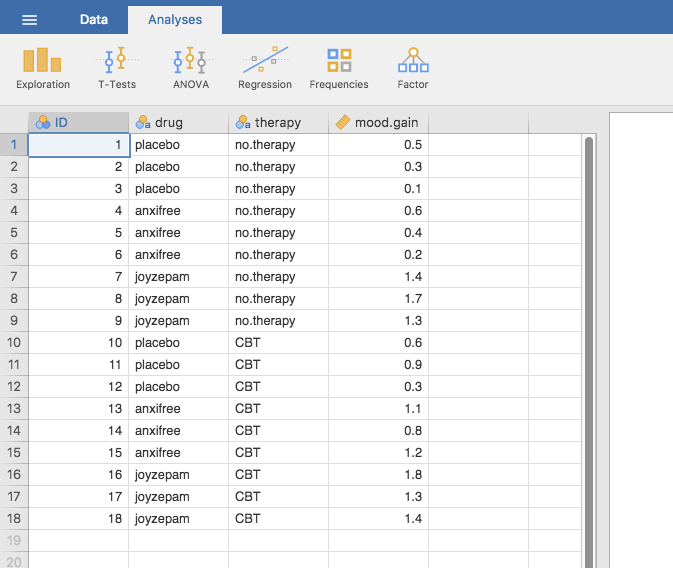
\includegraphics[width=9.35in]{img/descriptives/clinicaltrial} \caption{A screenshot of jamovi showing the variables stored in the clinicaltrial.csv file}\label{fig:clinicaltrial}
\end{figure}

Evidently there were three drugs: a placebo, something called ``anxifree'' and something called ``joyzepam'', and there were 6 people administered each drug. There were 9 people treated using cognitive behavioural therapy (CBT) and 9 people who received no psychological treatment. And we can see from looking at the `Descriptives' of the \texttt{mood.gain} variable that most people did show a mood gain (mean \(=0.88\)), though without knowing what the scale is here it's hard to say much more than that. Still, that's not too bad. Overall I feel that I learned something from that.

We can also go ahead and look at some other descriptive statistics, and this time separately for each type of therapy. In jamovi, check Std. deviation, Skewness and Kurtosis in the `Statistics' options. At the same time, transfer the \texttt{therapy} variable into the `Split by' box, and you should get something like Figure @ref(fig:clinicaltrial\_grouping)

\textbackslash begin\{figure\}
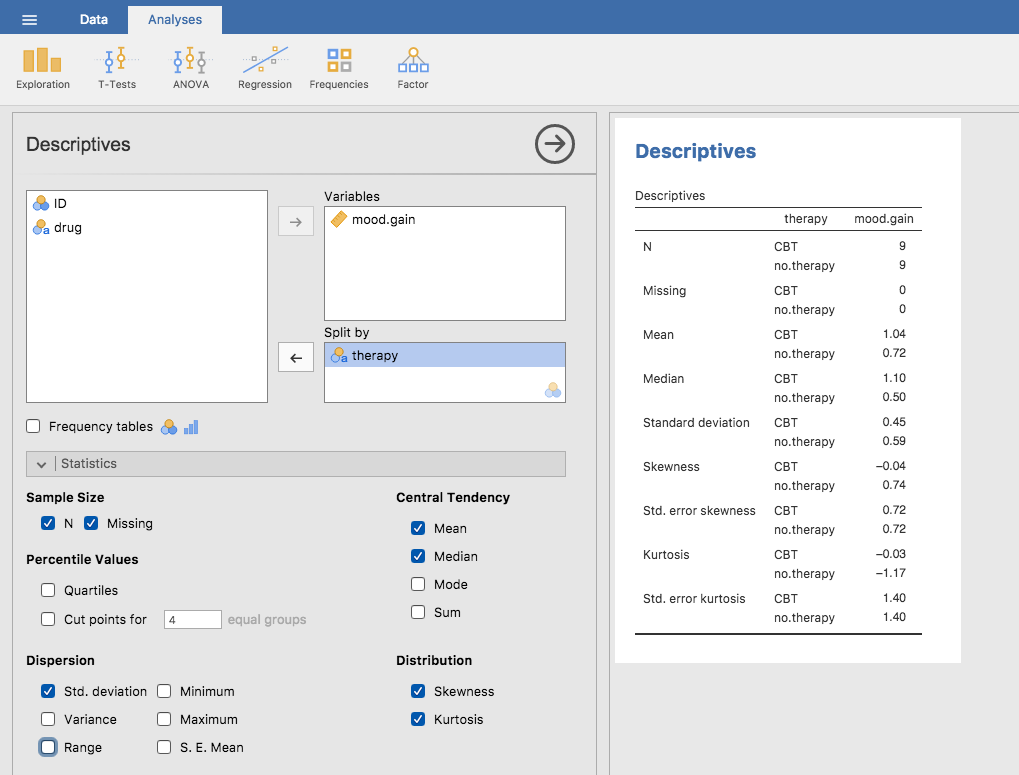
\includegraphics[width=14.15in]{img/descriptives/clinicaltrial_grouping}

\caption{A screenshot of jamovi showing Descriptives split by therapy type}

(\#fig:clinicaltrial\_grouping)
\textbackslash end\{figure\}

What if you have multiple grouping variables? Suppose you want to look at the average mood gain separately for all possible combinations of drug and therapy. It is possible to do this by adding another variable, \texttt{drug}, into the `Split by' box. Easy peasy, though sometimes if you split too much there isn't enough data in each breakdown combination to make meaningful calculations. In this case jamovi tells you this by stating something like \texttt{NaN} or \texttt{Inf}.\footnote{Sometimes jamovi will also present numbers in an unusual way. If a number is very small, or very large, then jamovi switches to an exponential form for numbers. For example \texttt{6.51e-4} is the same as saying that the decimal point is moved 4 places to the left, so the actual number is 0.000651. If there is a plus sign (i.e.~\texttt{6.51e+4} then the decimal point is moved to the right, i.e.~65,100.00. Usually only very small or very large numbers are expressed in this way, for example \texttt{6.51e-16}, which would be quite unwieldy to write out in the normal way.}

\hypertarget{zscore}{%
\section{Standard scores}\label{zscore}}

Suppose my friend is putting together a new questionnaire intended to measure ``grumpiness''. The survey has 50 questions which you can answer in a grumpy way or not. Across a big sample (hypothetically, let's imagine a million people or so!) the data are fairly normally distributed, with the mean grumpiness score being 17 out of 50 questions answered in a grumpy way, and the standard deviation is 5. In contrast, when I take the questionnaire I answer 35 out of 50 questions in a grumpy way. So, how grumpy am I? One way to think about it would be to say that I have grumpiness of 35/50, so you might say that I'm 70\% grumpy. But that's a bit weird, when you think about it. If my friend had phrased her questions a bit differently people might have answered them in a different way, so the overall distribution of answers could easily move up or down depending on the precise way in which the questions were asked. So, I'm only 70\% grumpy \emph{with respect to this set of survey questions}. Even if it's a very good questionnaire this isn't very a informative statement.

A simpler way around this is to describe my grumpiness by comparing me to other people. Shockingly, out of my friend's sample of 1,000,000 people, only 159 people were as grumpy as me (that's not at all unrealistic, frankly) suggesting that I'm in the top 0.016\% of people for grumpiness. This makes much more sense than trying to interpret the raw data. This idea, that we should describe my grumpiness in terms of the overall distribution of the grumpiness of humans, is the qualitative idea that standardisation attempts to get at. One way to do this is to do exactly what I just did and describe everything in terms of percentiles. However, the problem with doing this is that ``it's lonely at the top''. Suppose that my friend had only collected a sample of 1000 people (still a pretty big sample for the purposes of testing a new questionnaire, I'd like to add), and this time gotten, let's say, a mean of 16 out of 50 with a standard deviation of 5. The problem is that almost certainly not a single person in that sample would be as grumpy as me.

However, all is not lost. A different approach is to convert my grumpiness score into a \textbf{\emph{standard score}}, also referred to as a \(z\)-score. The standard score is defined as the number of standard deviations above the mean that my grumpiness score lies. To phrase it in ``pseudo-maths'' the standard score is calculated like this:
\[
\mbox{standard score} = \frac{\mbox{raw score} - \mbox{mean}}{\mbox{standard deviation}}
\]

In actual maths, the equation for the \(z\)-score is
\[
z_i = \frac{X_i - \bar{X}}{\hat\sigma}
\]

So, going back to the grumpiness data, we can now transform Dani's raw grumpiness into a standardised grumpiness score.
\[
z = \frac{35 - 17}{5} = 3.6
\]
To interpret this value, recall the rough heuristic that I provided in Section \ref{sec:sd} in which I noted that 99.7\% of values are expected to lie within 3 standard deviations of the mean. So the fact that my grumpiness corresponds to a \(z\) score of 3.6 indicates that I'm very grumpy indeed. In fact this suggests that I'm grumpier than 99.98\% of people. Sounds about right.

In addition to allowing you to interpret a raw score in relation to a larger population (and thereby allowing you to make sense of variables that lie on arbitrary scales), standard scores serve a second useful function. Standard scores can be compared to one another in situations where the raw scores can't. Suppose, for instance, my friend also had another questionnaire that measured extraversion using a 24 item questionnaire. The overall mean for this measure turns out to be 13 with standard deviation 4, and I scored a 2. As you can imagine, it doesn't make a lot of sense to try to compare my raw score of 2 on the extraversion questionnaire to my raw score of 35 on the grumpiness questionnaire. The raw scores for the two variables are ``about'' fundamentally different things, so this would be like comparing apples to oranges.

What about the standard scores? Well, this is a little different. If we calculate the standard scores we get \(z = (35-17)/5 = 3.6\) for grumpiness and \(z = (2-13)/4 = -2.75\) for extraversion. These two numbers \emph{can} be compared to each other.\footnote{Though some caution is usually warranted. It's not always the case that one standard deviation on variable A corresponds to the same ``kind'' of thing as one standard deviation on variable B. Use common sense when trying to determine whether or not the \(z\) scores of two variables can be meaningfully compared.} I'm much less extraverted than most people (\(z = -2.75\)) and much grumpier than most people (\(z = 3.6\)). But the extent of my unusualness is much more extreme for grumpiness, since 3.6 is a bigger number than 2.75. Because each standardised score is a statement about where an observation falls \emph{relative to its own population}, it \textbf{is} possible to compare standardised scores across completely different variables.

\hypertarget{summary}{%
\section{Summary}\label{summary}}

Calculating some basic descriptive statistics is one of the very first things you do when analysing real data, and descriptive statistics are much simpler to understand than inferential statistics, so like every other statistics textbook I've started with descriptives. In this chapter, we talked about the following topics:

\begin{itemize}
\tightlist
\item
  \emph{Measures of central tendency}. Broadly speaking, central tendency measures tell you where the data are. There's three measures that are typically reported in the literature: the mean, median and mode. (Section \ref{sec:centraltendency}
\item
  \emph{Measures of variability}. In contrast, measures of variability tell you about how ``spread out'' the data are. The key measures are: range, standard deviation, and interquartile range. (Section \ref{var}).
\item
  \emph{Measures of skewness and kurtosis}. We also looked at assymetry in a variable's distribution (skew) and pointness (kurtosis). (Section \ref{skewkurt})
\item
  \emph{Getting group summaries of variables in jamovi}. Since this book focuses on doing data analysis in jamovi, we spent a bit of time talking about how descriptive statistics are computed for different subgroups. (Section \ref{groupdescriptives}
\item
  \emph{Standard scores}. The \(z\)-score is a slightly unusual beast. It's not quite a descriptive statistic, and not quite an inference. We talked about it in Section \ref{sec:zscore}. Make sure you understand that section. It'll come up again later.
\end{itemize}

In the next Chapter we'll move on to a discussion of how to draw pictures! Everyone loves a pretty picture, right? But before we do, I want to end on an important point. A traditional first course in statistics spends only a small proportion of the class on descriptive statistics, maybe one or two lectures at most. The vast majority of the lecturer's time is spent on inferential statistics because that's where all the hard stuff is. That makes sense, but it hides the practical everyday importance of choosing good descriptives. With that in mind\ldots

\hypertarget{epilogue-good-descriptive-statistics-are-descriptive}{%
\subsection{Epilogue: Good descriptive statistics are descriptive!}\label{epilogue-good-descriptive-statistics-are-descriptive}}

\begin{quote}
\emph{The death of one man is a tragedy.}
\emph{The death of millions is a statistic.}

-- Josef Stalin, Potsdam 1945
\end{quote}

\begin{quote}
\emph{950,000 -- 1,200,000}

-- Estimate of Soviet repression deaths, 1937-1938 \citep{Ellman2002}
\end{quote}

Stalin's infamous quote about the statistical character of the deaths of millions is worth giving some thought. The clear intent of his statement is that the death of an individual touches us personally and its force cannot be denied, but that the deaths of a multitude are incomprehensible and as a consequence are mere statistics and more easily ignored. I'd argue that Stalin was half right. A statistic is an abstraction, a description of events beyond our personal experience, and so hard to visualise. Few if any of us can imagine what the deaths of millions is ``really'\,' like, but we can imagine one death and this gives the lone death its feeling of immediate tragedy, a feeling that is missing from Ellman's cold statistical description.

Yet it is not so simple. Without numbers, without counts, without a description of what happened, we have \emph{no chance} of understanding what really happened, no opportunity even to try to summon the missing feeling. And in truth, as I write this sitting in comfort on a Saturday morning half a world and a whole lifetime away from the Gulags, when I put the Ellman estimate next to the Stalin quote a dull dread settles in my stomach and a chill settles over me. The Stalinist repression is something truly beyond my experience, but with a combination of statistical data and those recorded personal histories that have come down to us, it is not entirely beyond my comprehension. Because what Ellman's numbers tell us is this: over a two year period Stalinist repression wiped out the equivalent of every man, woman and child currently alive in the city where I live. Each one of those deaths had it's own story, was it's own tragedy, and only some of those are known to us now. Even so, with a few carefully chosen statistics, the scale of the atrocity starts to come into focus.

Thus it is no small thing to say that the first task of the statistician and the scientist is to summarise the data, to find some collection of numbers that can convey to an audience a sense of what has happened. This is the job of descriptive statistics, but it's not a job that can be told solely using the numbers. You are a data analyst, and not a statistical software package. Part of your job is to take these \emph{statistics} and turn them into a \emph{description}. When you analyse data it is not sufficient to list off a collection of numbers. Always remember that what you're really trying to do is communicate with a human audience. The numbers are important, but they need to be put together into a meaningful story that your audience can interpret. That means you need to think about framing. You need to think about context. And you need to think about the individual events that your statistics are summarising.

  \bibliography{refs.bib}

\end{document}
